

\dangbt{Kiểm tra cặp số là nghiệm của bất phương trình/hệ bất phương trình bậc nhất hai ẩn}
\begin{ex}
% ID: T10C2B4-01-TN
% Mức: NB
 Cặp số nào sau đây là nghiệm của bất phương trình $x - 6 y - 4 > 0$.
 
\choice
{ $(1; 2)$ }
   { $(-4; 1)$ }
     { \True $(2; -10)$ }
    { $(4; 4)$ }
\loigiai{ 

 Thay các cặp số của các phương án vào ta thấy $(2; -10)$ thỏa mãn. 
 }\end{ex}

\begin{ex}
% ID: T10C2B4-02-TN
% Mức: NB
 Cặp số nào sau đây là nghiệm của bất phương trình $9 x + 3 y - 10 \ge 0$.
 
\choice
{ $(-10; -5)$ }
   { $(0; -7)$ }
     { \True $(-1; 7)$ }
    { $(-6; 6)$ }
\loigiai{ 

 Thay các cặp số của các phương án vào ta thấy $(-1; 7)$ thỏa mãn. 
 }\end{ex}

\begin{ex}
% ID: T10C2B4-03-TN
% Mức: NB
 Cặp số nào sau đây là nghiệm của bất phương trình $- 4 x + 5 y - 5 > 0$.
 
\choice
{ $(9; 7)$ }
   { $(9; -6)$ }
     { $(3; -10)$ }
    { \True $(-3; 8)$ }
\loigiai{ 

 Thay các cặp số của các phương án vào ta thấy $(-3; 8)$ thỏa mãn. 
 }\end{ex}

\begin{ex}
% ID: T10C2B4-04-TN
% Mức: NB
 Cặp số nào sau đây là nghiệm của bất phương trình $- 2 x + 10 y + 1 \ge 0$.
 
\choice
{ $(5; -7)$ }
   { $(6; -8)$ }
     { $(-2; -3)$ }
    { \True $(-1; 7)$ }
\loigiai{ 

 Thay các cặp số của các phương án vào ta thấy $(-1; 7)$ thỏa mãn. 
 }\end{ex}

\begin{ex}
% ID: T10C2B4-05-TN
% Mức: NB
 Cặp số nào sau đây là nghiệm của bất phương trình $- x + y - 1 \ge 0$.
 
\choice
{ $(1; -6)$ }
   { $(5; 2)$ }
     { $(-2; -3)$ }
    { \True $(-3; -1)$ }
\loigiai{ 

 Thay các cặp số của các phương án vào ta thấy $(-3; -1)$ thỏa mãn. 
 }\end{ex}

\begin{ex}
% ID: T10C2B4-06-TN
% Mức: NB
 Cặp số nào sau đây là nghiệm của bất phương trình $9 x - 6 y - 7 > 0$.
 
\choice
{ $(-7; -2)$ }
   { $(-7; -3)$ }
     { $(-4; -6)$ }
    { \True $(-2; -5)$ }
\loigiai{ 

 Thay các cặp số của các phương án vào ta thấy $(-2; -5)$ thỏa mãn. 
 }\end{ex}

\begin{ex}
% ID: T10C2B4-07-TN
% Mức: NB
 Cặp số nào sau đây là nghiệm của bất phương trình $- 5 x - 9 y + 6 > 0$.
 
\choice
{ \True $(-9; -10)$ }
   { $(-6; 8)$ }
     { $(8; -2)$ }
    { $(-6; 6)$ }
\loigiai{ 

 Thay các cặp số của các phương án vào ta thấy $(-9; -10)$ thỏa mãn. 
 }\end{ex}

\begin{ex}
% ID: T10C2B4-08-TN
% Mức: NB
 Cặp số nào sau đây là nghiệm của bất phương trình $- 6 x - y - 8 \ge 0$.
 
\choice
{ $(7; -5)$ }
   { \True $(-7; -4)$ }
     { $(7; -6)$ }
    { $(4; -3)$ }
\loigiai{ 

 Thay các cặp số của các phương án vào ta thấy $(-7; -4)$ thỏa mãn. 
 }\end{ex}

\begin{ex}
% ID: T10C2B4-09-TN
% Mức: NB
 Cặp số nào sau đây là nghiệm của bất phương trình $4 x - 4 y - 1 > 0$.
 
\choice
{ $(3; 9)$ }
   { $(3; 3)$ }
     { $(-5; 7)$ }
    { \True $(1; -6)$ }
\loigiai{ 

 Thay các cặp số của các phương án vào ta thấy $(1; -6)$ thỏa mãn. 
 }\end{ex}

\begin{ex}
% ID: T10C2B4-10-TN
% Mức: NB
 Cặp số nào sau đây là nghiệm của bất phương trình $4 x + 3 y - 9 > 0$.
 
\choice
{ $(-3; 0)$ }
   { $(0; 2)$ }
     { \True $(2; 5)$ }
    { $(-7; -7)$ }
\loigiai{ 

 Thay các cặp số của các phương án vào ta thấy $(2; 5)$ thỏa mãn. 
 }\end{ex}

\begin{ex}
% ID: T10C2B4-11-TN
% Mức: NB
 Cặp số nào sau đây là nghiệm của bất phương trình $- x - 5 y - 4 \le 0$.

 
\choice
{ \True $(-7; 7)$ }
   { $(-2; -6)$ }
     { $(-2; -1)$ }
    { $(7; -5)$ }
\loigiai{ 

 Thay các cặp số của các phương án vào ta thấy $(-7; 7)$ thỏa mãn. 
 }\end{ex}

\begin{ex}
% ID: T10C2B4-12-TN
% Mức: NB
 Cặp số nào sau đây là nghiệm của bất phương trình $9 x - 10 y + 10 \le 0$.

 
\choice
{ $(7; 0)$ }
   { $(4; 4)$ }
     { $(-1; -2)$ }
    { \True $(2; 5)$ }
\loigiai{ 

 Thay các cặp số của các phương án vào ta thấy $(2; 5)$ thỏa mãn. 
 }\end{ex}

\begin{ex}
% ID: T10C2B4-13-TN
% Mức: NB
 Cặp số nào sau đây là nghiệm của bất phương trình $6 x - 7 y - 8 \le 0$.

 
\choice
{ $(3; 0)$ }
   { $(0; -7)$ }
     { \True $(-5; 2)$ }
    { $(4; -5)$ }
\loigiai{ 

 Thay các cặp số của các phương án vào ta thấy $(-5; 2)$ thỏa mãn. 
 }\end{ex}

\begin{ex}
% ID: T10C2B4-14-TN
% Mức: NB
 Cặp số nào sau đây là nghiệm của bất phương trình $- 4 x + 5 y - 8 \le 0$.

 
\choice
{ \True $(-5; -4)$ }
   { $(-9; 4)$ }
     { $(-10; 0)$ }
    { $(-5; 7)$ }
\loigiai{ 

 Thay các cặp số của các phương án vào ta thấy $(-5; -4)$ thỏa mãn. 
 }\end{ex}

\begin{ex}
% ID: T10C2B4-15-TN
% Mức: NB
 Cặp số nào sau đây là nghiệm của bất phương trình $- x - 4 y + 10 \le 0$.

 
\choice
{ \True $(5; 3)$ }
   { $(-8; -7)$ }
     { $(-3; -6)$ }
    { $(-7; 2)$ }
\loigiai{ 

 Thay các cặp số của các phương án vào ta thấy $(5; 3)$ thỏa mãn. 
 }\end{ex}

\begin{ex}
% ID: T10C2B4-16-TN
% Mức: NB
 Cặp số nào sau đây là nghiệm của bất phương trình $- 6 x + 7 y - 1 \le 0$.

 
\choice
{ $(-9; 0)$ }
   { $(-4; 4)$ }
     { \True $(-4; -6)$ }
    { $(1; 3)$ }
\loigiai{ 

 Thay các cặp số của các phương án vào ta thấy $(-4; -6)$ thỏa mãn. 
 }\end{ex}

\begin{ex}
% ID: T10C2B4-17-TN
% Mức: NB
 Cặp số nào sau đây là nghiệm của bất phương trình $- 6 x - 9 y - 3 \le 0$.

 
\choice
{ $(-9; -5)$ }
   { $(-9; -9)$ }
     { $(-10; -6)$ }
    { \True $(-9; 7)$ }
\loigiai{ 

 Thay các cặp số của các phương án vào ta thấy $(-9; 7)$ thỏa mãn. 
 }\end{ex}

\begin{ex}
% ID: T10C2B4-18-TN
% Mức: NB
 Cặp số nào sau đây là nghiệm của bất phương trình $- 4 x + 2 y + 8 < 0$.

 
\choice
{ $(0; -1)$ }
   { $(-9; 9)$ }
     { $(-8; 8)$ }
    { \True $(7; -8)$ }
\loigiai{ 

 Thay các cặp số của các phương án vào ta thấy $(7; -8)$ thỏa mãn. 
 }\end{ex}

\begin{ex}
% ID: T10C2B4-19-TN
% Mức: NB
 Cặp số nào sau đây là nghiệm của bất phương trình $5 x + 5 y - 3 < 0$.

 
\choice
{ $(5; 2)$ }
   { \True $(-8; 0)$ }
     { $(2; -1)$ }
    { $(7; 6)$ }
\loigiai{ 

 Thay các cặp số của các phương án vào ta thấy $(-8; 0)$ thỏa mãn. 
 }\end{ex}

\begin{ex}
% ID: T10C2B4-20-TN
% Mức: NB
 Cặp số nào sau đây là nghiệm của bất phương trình $- x + 6 y + 9 < 0$.

 
\choice
{ \True $(6; -8)$ }
   { $(-6; -1)$ }
     { $(8; 0)$ }
    { $(3; 5)$ }
\loigiai{ 

 Thay các cặp số của các phương án vào ta thấy $(6; -8)$ thỏa mãn. 
 }\end{ex}



\dangbt{Lập bất phương trình/hệ bất phương trình bậc nhất hai ẩn từ bài toán thực tế}
\begin{ex}
% ID: T10C2B4-21-TN
% Mức: NB
 Bất phương trình nào sau đây là bất phương trình bậc nhất hai ẩn\ 
\choice
{ \True $- 8 x + 6 y\le -10$ }
   { $- 7 x^{2} - 7 y - 8 \le 0$ }
     { $-2 - \frac{10}{y} - \frac{8}{x} \ge 0$ }
    { $8 x^{2} + 4 y^{2} < 5$ }
\loigiai{ 
 $- 8 x + 6 y\le -10$ là bất phương trình bậc nhất 2 ẩn. 
 }\end{ex}

\begin{ex}
% ID: T10C2B4-22-TN
% Mức: NB
 Bất phương trình nào sau đây là bất phương trình bậc nhất hai ẩn\ 
\choice
{ $3 x^{2} + 8 y^{2} \le -5$ }
   { $2 x^{2} - 8 y + 4 < 0$ }
     { \True $6 x - 4 y - 7\ge 0$ }
    { $-1 + \frac{9}{y} + \frac{8}{x} \ge 0$ }
\loigiai{ 
 $6 x - 4 y - 7\ge 0$ là bất phương trình bậc nhất 2 ẩn. 
 }\end{ex}

\begin{ex}
% ID: T10C2B4-23-TN
% Mức: NB
 Bất phương trình nào sau đây là bất phương trình bậc nhất hai ẩn\ 
\choice
{ $- 3 x^{2} + y^{2} > -10$ }
   { $x^{2} + 4 y + 2 < 0$ }
     { $-6 + \frac{5}{y} + \frac{6}{x} \ge 0$ }
    { \True $- 4 x - 2 y> -5$ }
\loigiai{ 
 $- 4 x - 2 y> -5$ là bất phương trình bậc nhất 2 ẩn. 
 }\end{ex}

\begin{ex}
% ID: T10C2B4-24-TN
% Mức: NB
 Bất phương trình nào sau đây là bất phương trình bậc nhất hai ẩn\ 
\choice
{ $8 x^{2} + 5 y + 4 < 0$ }
   { \True $8 x - 10 y\ge 9$ }
     { $- x^{2} - y^{2} \ge 0$ }
    { $4 + \frac{7}{y} + \frac{8}{x} \ge 0$ }
\loigiai{ 
 $8 x - 10 y\ge 9$ là bất phương trình bậc nhất 2 ẩn. 
 }\end{ex}

\begin{ex}
% ID: T10C2B4-25-TN
% Mức: NB
 Bất phương trình nào sau đây là bất phương trình bậc nhất hai ẩn\ 
\choice
{ $- 9 x^{2} + y^{2} < 8$ }
   { $- x^{2} + 8 y - 5 > 0$ }
     { $-8 - \frac{9}{y} - \frac{7}{x} < 0$ }
    { \True $- x + 7 y\ge 2$ }
\loigiai{ 
 $- x + 7 y\ge 2$ là bất phương trình bậc nhất 2 ẩn. 
 }\end{ex}

\begin{ex}
% ID: T10C2B4-26-TN
% Mức: NB
 Bất phương trình nào sau đây là bất phương trình bậc nhất hai ẩn\ 
\choice
{ $-7 - \frac{8}{y} - \frac{9}{x} < 0$ }
   { $- 6 x^{2} - 10 y - 4 < 0$ }
     { \True $- 3 x - 8 y - 2\ge 0$ }
    { $- 8 x^{2} + 7 y^{2} < -6$ }
\loigiai{ 
 $- 3 x - 8 y - 2\ge 0$ là bất phương trình bậc nhất 2 ẩn. 
 }\end{ex}

\begin{ex}
% ID: T10C2B4-27-TN
% Mức: NB
 Bất phương trình nào sau đây là bất phương trình bậc nhất hai ẩn\ 
\choice
{ $- 8 x^{2} + 8 y^{2} < -1$ }
   { $-10 - \frac{5}{y} + \frac{2}{x} \le 0$ }
     { \True $- 8 x + y - 6\ge 0$ }
    { $8 x^{2} - 4 y + 7 > 0$ }
\loigiai{ 
 $- 8 x + y - 6\ge 0$ là bất phương trình bậc nhất 2 ẩn. 
 }\end{ex}

\begin{ex}
% ID: T10C2B4-28-TN
% Mức: NB
 Bất phương trình nào sau đây là bất phương trình bậc nhất hai ẩn\ 
\choice
{ \True $7 x - 6 y - 9\ge 0$ }
   { $7 x^{2} + 9 y^{2} < -4$ }
     { $x^{2} - 5 y - 3 < 0$ }
    { $-9 - \frac{7}{y} - \frac{5}{x} \ge 0$ }
\loigiai{ 
 $7 x - 6 y - 9\ge 0$ là bất phương trình bậc nhất 2 ẩn. 
 }\end{ex}

\begin{ex}
% ID: T10C2B4-29-TN
% Mức: NB
 Bất phương trình nào sau đây là bất phương trình bậc nhất hai ẩn\ 
\choice
{ \True $6 x - 2 y< 9$ }
   { $7 x^{2} - 3 y + 6 < 0$ }
     { $-2 + \frac{5}{y} - \frac{5}{x} > 0$ }
    { $x^{2} - 9 y^{2} > 9$ }
\loigiai{ 
 $6 x - 2 y< 9$ là bất phương trình bậc nhất 2 ẩn. 
 }\end{ex}

\begin{ex}
% ID: T10C2B4-30-TN
% Mức: NB
 Bất phương trình nào sau đây là bất phương trình bậc nhất hai ẩn\ 
\choice
{ \True $- 3 x + 8 y\le 3$ }
   { $- 5 x^{2} - 8 y + 1 > 0$ }
     { $- 3 x^{2} + 9 y^{2} < -7$ }
    { $-2 + \frac{1}{y} + \frac{9}{x} > 0$ }
\loigiai{ 
 $- 3 x + 8 y\le 3$ là bất phương trình bậc nhất 2 ẩn. 
 }\end{ex}



\dangbt{Xác định miền nghiệm của bất phương trình/hệ bất phương trình bậc nhất hai ẩn}
\begin{ex}
% ID: T10C2B4-31-TN
% Mức: TH
 Miền nghiệm của bất phương trình $- 2 x + y\le -5$ là nửa mặt phẳng chứa điểm nào trong các điểm sau?\ 
\choice
{ $(-9; -3)$ }
   { $(-5; -6)$ }
     { $(-4; -10)$ }
    { \True $(6; -10)$ }
\loigiai{ 
 Thay $(6; -10)$ vào bất phương trình thấy thỏa mãn nên miền nghiệm là nửa mặt phẳng chứa điểm $(6; -10)$. 
 }\end{ex}

\begin{ex}
% ID: T10C2B4-32-TN
% Mức: TH
 Miền nghiệm của bất phương trình $4 x + 2 y\le 2$ là nửa mặt phẳng chứa điểm nào trong các điểm sau?\ 
\choice
{ \True $(-8; -9)$ }
   { $(2; -1)$ }
     { $(8; -4)$ }
    { $(9; 9)$ }
\loigiai{ 
 Thay $(-8; -9)$ vào bất phương trình thấy thỏa mãn nên miền nghiệm là nửa mặt phẳng chứa điểm $(-8; -9)$. 
 }\end{ex}

\begin{ex}
% ID: T10C2B4-33-TN
% Mức: TH
 Miền nghiệm của bất phương trình $- 5 x + 4 y - 6< 0$ là nửa mặt phẳng chứa điểm nào trong các điểm sau?\ 
\choice
{ $(-4; 4)$ }
   { $(-9; -4)$ }
     { $(-4; 9)$ }
    { \True $(5; -9)$ }
\loigiai{ 
 Thay $(5; -9)$ vào bất phương trình thấy thỏa mãn nên miền nghiệm là nửa mặt phẳng chứa điểm $(5; -9)$. 
 }\end{ex}

\begin{ex}
% ID: T10C2B4-34-TN
% Mức: TH
 Miền nghiệm của bất phương trình $2 x + 4 y + 2\le 0$ là nửa mặt phẳng chứa điểm nào trong các điểm sau?\ 
\choice
{ $(-8; 9)$ }
   { $(5; 2)$ }
     { \True $(-7; -7)$ }
    { $(-7; 4)$ }
\loigiai{ 
 Thay $(-7; -7)$ vào bất phương trình thấy thỏa mãn nên miền nghiệm là nửa mặt phẳng chứa điểm $(-7; -7)$. 
 }\end{ex}

\begin{ex}
% ID: T10C2B4-35-TN
% Mức: TH
 Miền nghiệm của bất phương trình $- 3 x + 2 y< 2$ là nửa mặt phẳng chứa điểm nào trong các điểm sau?\ 
\choice
{ $(-10; -5)$ }
   { \True $(6; 3)$ }
     { $(-3; 6)$ }
    { $(-3; 5)$ }
\loigiai{ 
 Thay $(6; 3)$ vào bất phương trình thấy thỏa mãn nên miền nghiệm là nửa mặt phẳng chứa điểm $(6; 3)$. 
 }\end{ex}

\begin{ex}
% ID: T10C2B4-36-TN
% Mức: TH
 Miền nghiệm của bất phương trình $4 x + y< -1$ là nửa mặt phẳng chứa điểm nào trong các điểm sau?\ 
\choice
{ $(8; 3)$ }
   { $(5; 5)$ }
     { \True $(-6; -3)$ }
    { $(2; 3)$ }
\loigiai{ 
 Thay $(-6; -3)$ vào bất phương trình thấy thỏa mãn nên miền nghiệm là nửa mặt phẳng chứa điểm $(-6; -3)$. 
 }\end{ex}

\begin{ex}
% ID: T10C2B4-37-TN
% Mức: TH
 Miền nghiệm của bất phương trình $- 2 x + 3 y> -5$ là nửa mặt phẳng chứa điểm nào\ 
\choice
{ \True $(-2; 5)$ }
   { $(-4; -8)$ }
     { $(9; 0)$ }
    { $(7; -3)$ }
\loigiai{ 
 Thay $(-2; 5)$ vào bất phương trình thấy thỏa mãn nên miền nghiệm là nửa mặt phẳng chứa điểm $(-2; 5)$. 
 }\end{ex}

\begin{ex}
% ID: T10C2B4-38-TN
% Mức: TH
 Miền nghiệm của bất phương trình $- x + 2 y< -3$ là nửa mặt phẳng chứa điểm nào trong các điểm sau?\ 
\choice
{ $(-6; 5)$ }
   { $(-6; 7)$ }
     { $(-1; 3)$ }
    { \True $(5; -3)$ }
\loigiai{ 
 Thay $(5; -3)$ vào bất phương trình thấy thỏa mãn nên miền nghiệm là nửa mặt phẳng chứa điểm $(5; -3)$. 
 }\end{ex}

\begin{ex}
% ID: T10C2B4-39-TN
% Mức: TH
 Miền nghiệm của bất phương trình $- 4 x + 3 y - 4< 0$ là nửa mặt phẳng chứa điểm nào trong các điểm sau?\ 
\choice
{ \True $(4; -9)$ }
   { $(0; 8)$ }
     { $(-8; 2)$ }
    { $(-3; 6)$ }
\loigiai{ 
 Thay $(4; -9)$ vào bất phương trình thấy thỏa mãn nên miền nghiệm là nửa mặt phẳng chứa điểm $(4; -9)$. 
 }\end{ex}

\begin{ex}
% ID: T10C2B4-40-TN
% Mức: TH
 Miền nghiệm của bất phương trình $3 x + 4 y> 1$ là nửa mặt phẳng chứa điểm nào\ 
\choice
{ \True $(5; 4)$ }
   { $(-5; -6)$ }
     { $(-3; -6)$ }
    { $(1; -8)$ }
\loigiai{ 
 Thay $(5; 4)$ vào bất phương trình thấy thỏa mãn nên miền nghiệm là nửa mặt phẳng chứa điểm $(5; 4)$. 
 }\end{ex}

\begin{ex}
% ID: T10C2B4-41-TN
% Mức: TH
 Miền nghiệm của bất phương trình $- 4 x + 6 y + 8\ge - 3 x + 3 y + 1$ là nửa mặt phẳng chứa điểm nào
\choice
{ $(6; -6)$ }
   { \True $(-5; -2)$ }
     { $(0; -8)$ }
    { $(6; -1)$ }
\loigiai{ 
 Thay $(-5; -2)$ vào bất phương trình thấy thỏa mãn nên miền nghiệm là nửa mặt phẳng chứa điểm $(-5; -2)$. 
 }\end{ex}

\begin{ex}
% ID: T10C2B4-42-TN
% Mức: TH
 Miền nghiệm của bất phương trình $- 3 x + 3 y + 7\le - 2 x + y + 9$ là nửa mặt phẳng chứa điểm nào trong các điểm sau?
\choice
{ $(-2; 3)$ }
   { \True $(9; 3)$ }
     { $(4; 7)$ }
    { $(0; 8)$ }
\loigiai{ 
 Thay $(9; 3)$ vào bất phương trình thấy thỏa mãn nên miền nghiệm là nửa mặt phẳng chứa điểm $(9; 3)$. 
 }\end{ex}

\begin{ex}
% ID: T10C2B4-43-TN
% Mức: TH
 Miền nghiệm của bất phương trình $- 8 x + 3 y - 2\le - 5 x + 2 y + 2$ là nửa mặt phẳng chứa điểm nào trong các điểm sau?
\choice
{ $(-9; -9)$ }
   { $(-9; 3)$ }
     { \True $(-1; -7)$ }
    { $(-6; -10)$ }
\loigiai{ 
 Thay $(-1; -7)$ vào bất phương trình thấy thỏa mãn nên miền nghiệm là nửa mặt phẳng chứa điểm $(-1; -7)$. 
 }\end{ex}

\begin{ex}
% ID: T10C2B4-44-TN
% Mức: TH
 Miền nghiệm của bất phương trình $- x + 5 y + 10\le - 5 x + 3 y + 6$ là nửa mặt phẳng chứa điểm nào trong các điểm sau?
\choice
{ $(2; 5)$ }
   { $(9; 0)$ }
     { \True $(-3; 1)$ }
    { $(9; -9)$ }
\loigiai{ 
 Thay $(-3; 1)$ vào bất phương trình thấy thỏa mãn nên miền nghiệm là nửa mặt phẳng chứa điểm $(-3; 1)$. 
 }\end{ex}

\begin{ex}
% ID: T10C2B4-45-TN
% Mức: TH
 Miền nghiệm của bất phương trình $x + 6 y + 16\ge 2 x + 4 y + 7$ là nửa mặt phẳng chứa điểm nào
\choice
{ $(-7; -10)$ }
   { $(2; -7)$ }
     { $(3; -5)$ }
    { \True $(1; -2)$ }
\loigiai{ 
 Thay $(1; -2)$ vào bất phương trình thấy thỏa mãn nên miền nghiệm là nửa mặt phẳng chứa điểm $(1; -2)$. 
 }\end{ex}

\begin{ex}
% ID: T10C2B4-46-TN
% Mức: TH
 Miền nghiệm của bất phương trình $8 x + 2 y + 1< 4 x + y + 2$ là nửa mặt phẳng chứa điểm nào trong các điểm sau?
\choice
{ $(9; -3)$ }
   { $(6; 6)$ }
     { $(7; 2)$ }
    { \True $(-7; 0)$ }
\loigiai{ 
 Thay $(-7; 0)$ vào bất phương trình thấy thỏa mãn nên miền nghiệm là nửa mặt phẳng chứa điểm $(-7; 0)$. 
 }\end{ex}

\begin{ex}
% ID: T10C2B4-47-TN
% Mức: TH
 Miền nghiệm của bất phương trình $4 x + 5 y + 12< 2 x + 3 y + 3$ là nửa mặt phẳng chứa điểm nào trong các điểm sau?
\choice
{ $(5; 1)$ }
   { $(0; 9)$ }
     { \True $(1; -6)$ }
    { $(-5; 2)$ }
\loigiai{ 
 Thay $(1; -6)$ vào bất phương trình thấy thỏa mãn nên miền nghiệm là nửa mặt phẳng chứa điểm $(1; -6)$. 
 }\end{ex}

\begin{ex}
% ID: T10C2B4-48-TN
% Mức: TH
 Miền nghiệm của bất phương trình $- 7 x + 5 y + 3> - 4 x + y + 5$ là nửa mặt phẳng chứa điểm nào
\choice
{ $(4; -7)$ }
   { $(2; -9)$ }
     { $(7; -4)$ }
    { \True $(-8; 4)$ }
\loigiai{ 
 Thay $(-8; 4)$ vào bất phương trình thấy thỏa mãn nên miền nghiệm là nửa mặt phẳng chứa điểm $(-8; 4)$. 
 }\end{ex}

\begin{ex}
% ID: T10C2B4-49-TN
% Mức: TH
 Miền nghiệm của bất phương trình $- 2 x + 5 y - 4< 3 x + 4 y + 2$ là nửa mặt phẳng chứa điểm nào trong các điểm sau?
\choice
{ $(-3; -4)$ }
   { \True $(6; -1)$ }
     { $(-5; 0)$ }
    { $(-7; 7)$ }
\loigiai{ 
 Thay $(6; -1)$ vào bất phương trình thấy thỏa mãn nên miền nghiệm là nửa mặt phẳng chứa điểm $(6; -1)$. 
 }\end{ex}

\begin{ex}
% ID: T10C2B4-50-TN
% Mức: TH
 Miền nghiệm của bất phương trình $- 9 x + 8 y + 9< - 4 x + 4 y + 1$ là nửa mặt phẳng chứa điểm nào trong các điểm sau?
\choice
{ \True $(6; -4)$ }
   { $(-7; -9)$ }
     { $(2; 1)$ }
    { $(-10; 3)$ }
\loigiai{ 
 Thay $(6; -4)$ vào bất phương trình thấy thỏa mãn nên miền nghiệm là nửa mặt phẳng chứa điểm $(6; -4)$. 
 }\end{ex}


\begin{ex}
% ID: T10C2B4-51-TN
% Mức: TH
 Cặp số $(x;y)$ nào sau đây là nghiệm của bất phương trình có miền nghiệm là nửa mặt phẳng không bị gạch có bờ là đường thẳng $d$ như hình bên?\ 
\begin{center}
 \begin{tikzpicture}[line join=round, line cap=round,>=stealth,thick]
    \tikzset{every node/.style={scale=0.9}}
    \begin{scope}
        \clip (-4,-3) rectangle (3.2,4.2);
        \fill[pattern=north east lines] (-4,-5)--(-4,4)--(3,4)--(3,2)--cycle;
        \draw [blue, thick](-4,-5)--(3,2);
    \end{scope}
    \draw[->] (-4,0)--(3.2,0);
    \draw(3.2,0) node[below]{$x$};
    \draw(0,4.2) node[above]{$y$};
    \draw[->] (0,-3)--(0,4.2);
    \draw (0,0) node[below left]{$O$};
    \foreach \x in {-1,-2,1,2}
    \draw[thin] (\x,1pt)--(\x,-1pt) node [below] {$\x$};
    \foreach \y in {-1,-2,1,2}
    \draw[thin] (1pt,\y)--(-1pt,\y) node [left] {$\y$};
\end{tikzpicture}
\end{center}
\choice
{ $(-3; 1)$ }
   { $(4; 4)$ }
     { \True $(8; 1)$ }
    { $(6; 8)$ }
\loigiai{ 
 Dựa vào hình vẽ ta thấy $(8; 1)$ thuộc miền nghiệm nên $(8; 1)$ là nghiệm của bất phương trình. 
 }\end{ex}

\begin{ex}
% ID: T10C2B4-52-TN
% Mức: TH
 Cặp số $(x;y)$ nào sau đây là nghiệm của bất phương trình có miền nghiệm là nửa mặt phẳng không bị gạch có bờ là đường thẳng $d$ như hình bên?\ 
\begin{center}
 \begin{tikzpicture}[line join=round, line cap=round,>=stealth,thick]
    \tikzset{every node/.style={scale=0.9}}
    \begin{scope}
        \clip (-4,-4) rectangle (2.2,4.2);
        \fill[pattern=north east lines] (-4,-14)--(-4,-4)--(2,-4)--(2,4)--cycle;
        \draw [blue, thick](-4,-14)--(2,4);
    \end{scope}
    \draw[->] (-4,0)--(2.2,0);
    \draw(2.2,0) node[below]{$x$};
    \draw(0,4.2) node[above]{$y$};
    \draw[->] (0,-4)--(0,4.2);
    \draw (0,0) node[below left]{$O$};
    \foreach \x in {-1,-2,1,2}
    \draw[thin] (\x,1pt)--(\x,-1pt) node [below] {$\x$};
    \foreach \y in {-1,-2,1,2}
    \draw[thin] (1pt,\y)--(-1pt,\y) node [left] {$\y$};
\end{tikzpicture}
\end{center}
\choice
{ $(8; 2)$ }
   { $(6; 9)$ }
     { $(5; -8)$ }
    { \True $(-5; -3)$ }
\loigiai{ 
 Dựa vào hình vẽ ta thấy $(-5; -3)$ thuộc miền nghiệm nên $(-5; -3)$ là nghiệm của bất phương trình. 
 }\end{ex}

\begin{ex}
% ID: T10C2B4-53-TN
% Mức: TH
 Cặp số $(x;y)$ nào sau đây là nghiệm của bất phương trình có miền nghiệm là nửa mặt phẳng không bị gạch có bờ là đường thẳng $d$ như hình bên?\ 
\begin{center}
 \begin{tikzpicture}[line join=round, line cap=round,>=stealth,thick]
    \tikzset{every node/.style={scale=0.9}}
    \begin{scope}
        \clip (-4,-2) rectangle (3.2,4.2);
        \fill[pattern=north east lines] (-4,-10/3)--(-4,4)--(3,4)--(3,4/3)--cycle;
        \draw [blue, thick](-4,-10/3)--(3,4/3);
    \end{scope}
    \draw[->] (-4,0)--(3.2,0);
    \draw(3.2,0) node[below]{$x$};
    \draw(0,4.2) node[above]{$y$};
    \draw[->] (0,-2)--(0,4.2);
    \draw (0,0) node[below left]{$O$};
    \foreach \x in {-1,-2,1,2}
    \draw[thin] (\x,1pt)--(\x,-1pt) node [below] {$\x$};
    \foreach \y in {-1,-2,1,2}
    \draw[thin] (1pt,\y)--(-1pt,\y) node [left] {$\y$};
\end{tikzpicture}
\end{center}
\choice
{ $(1; 2)$ }
   { \True $(-2; -8)$ }
     { $(-7; -3)$ }
    { $(-3; 1)$ }
\loigiai{ 
 Dựa vào hình vẽ ta thấy $(-2; -8)$ thuộc miền nghiệm nên $(-2; -8)$ là nghiệm của bất phương trình. 
 }\end{ex}

\begin{ex}
% ID: T10C2B4-54-TN
% Mức: TH
 Cặp số $(x;y)$ nào sau đây là nghiệm của bất phương trình có miền nghiệm là nửa mặt phẳng không bị gạch có bờ là đường thẳng $d$ như hình bên?\ 
\begin{center}
 \begin{tikzpicture}[line join=round, line cap=round,>=stealth,thick]
    \tikzset{every node/.style={scale=0.9}}
    \begin{scope}
        \clip (-4,-3) rectangle (3.2,4.2);
        \fill[pattern=north east lines] (-4,-5)--(-4,4)--(3,4)--(3,2)--cycle;
        \draw [blue, thick](-4,-5)--(3,2);
    \end{scope}
    \draw[->] (-4,0)--(3.2,0);
    \draw(3.2,0) node[below]{$x$};
    \draw(0,4.2) node[above]{$y$};
    \draw[->] (0,-3)--(0,4.2);
    \draw (0,0) node[below left]{$O$};
    \foreach \x in {-1,-2,1,2}
    \draw[thin] (\x,1pt)--(\x,-1pt) node [below] {$\x$};
    \foreach \y in {-1,-2,1,2}
    \draw[thin] (1pt,\y)--(-1pt,\y) node [left] {$\y$};
\end{tikzpicture}
\end{center}
\choice
{ $(-2; 9)$ }
   { $(-7; -4)$ }
     { \True $(8; 1)$ }
    { $(-3; -1)$ }
\loigiai{ 
 Dựa vào hình vẽ ta thấy $(8; 1)$ thuộc miền nghiệm nên $(8; 1)$ là nghiệm của bất phương trình. 
 }\end{ex}

\begin{ex}
% ID: T10C2B4-55-TN
% Mức: TH
 Cặp số $(x;y)$ nào sau đây là nghiệm của bất phương trình có miền nghiệm là nửa mặt phẳng không bị gạch có bờ là đường thẳng $d$ như hình bên?\ 
\begin{center}
 \begin{tikzpicture}[line join=round, line cap=round,>=stealth,thick]
    \tikzset{every node/.style={scale=0.9}}
    \begin{scope}
        \clip (-4,-2) rectangle (3.2,4.2);
        \fill[pattern=north east lines] (-4,-10/3)--(-4,4)--(3,4)--(3,4/3)--cycle;
        \draw [blue, thick](-4,-10/3)--(3,4/3);
    \end{scope}
    \draw[->] (-4,0)--(3.2,0);
    \draw(3.2,0) node[below]{$x$};
    \draw(0,4.2) node[above]{$y$};
    \draw[->] (0,-2)--(0,4.2);
    \draw (0,0) node[below left]{$O$};
    \foreach \x in {-1,-2,1,2}
    \draw[thin] (\x,1pt)--(\x,-1pt) node [below] {$\x$};
    \foreach \y in {-1,-2,1,2}
    \draw[thin] (1pt,\y)--(-1pt,\y) node [left] {$\y$};
\end{tikzpicture}
\end{center}
\choice
{ $(-8; 3)$ }
   { \True $(-9; -7)$ }
     { $(4; 6)$ }
    { $(0; 6)$ }
\loigiai{ 
 Dựa vào hình vẽ ta thấy $(-9; -7)$ thuộc miền nghiệm nên $(-9; -7)$ là nghiệm của bất phương trình. 
 }\end{ex}

\begin{ex}
% ID: T10C2B4-56-TN
% Mức: TH
 Cặp số $(x;y)$ nào sau đây là nghiệm của bất phương trình có miền nghiệm là nửa mặt phẳng không bị gạch có bờ là đường thẳng $d$ như hình bên?\ 
\begin{center}
 \begin{tikzpicture}[line join=round, line cap=round,>=stealth,thick]
    \tikzset{every node/.style={scale=0.9}}
    \begin{scope}
        \clip (-3,-3) rectangle (4.2,4.2);
        \fill[pattern=north east lines] (-3,1)--(-3,4)--(4,4)--(4,-11/3)--cycle;
        \draw [blue, thick](-3,1)--(4,-11/3);
    \end{scope}
    \draw[->] (-3,0)--(4.2,0);
    \draw(4.2,0) node[below]{$x$};
    \draw(0,4.2) node[above]{$y$};
    \draw[->] (0,-3)--(0,4.2);
    \draw (0,0) node[below left]{$O$};
    \foreach \x in {-1,-2,1,2}
    \draw[thin] (\x,1pt)--(\x,-1pt) node [below] {$\x$};
    \foreach \y in {-1,-2,1,2}
    \draw[thin] (1pt,\y)--(-1pt,\y) node [left] {$\y$};
\end{tikzpicture}
\end{center}
\choice
{ $(6; -3)$ }
   { $(8; 8)$ }
     { $(-5; 7)$ }
    { \True $(-8; -5)$ }
\loigiai{ 
 Dựa vào hình vẽ ta thấy $(-8; -5)$ thuộc miền nghiệm nên $(-8; -5)$ là nghiệm của bất phương trình. 
 }\end{ex}

\begin{ex}
% ID: T10C2B4-57-TN
% Mức: TH
 Cặp số $(x;y)$ nào sau đây là nghiệm của bất phương trình có miền nghiệm là nửa mặt phẳng không bị gạch có bờ là đường thẳng $d$ như hình bên?\ 
\begin{center}
 \begin{tikzpicture}[line join=round, line cap=round,>=stealth,thick]
    \tikzset{every node/.style={scale=0.9}}
    \begin{scope}
        \clip (-4,-4) rectangle (3.2,3.2);
        \fill[pattern=north east lines] (-4,5)--(-4,-4)--(3,-4)--(3,-2)--cycle;
        \draw [blue, thick](-4,5)--(3,-2);
    \end{scope}
    \draw[->] (-4,0)--(3.2,0);
    \draw(3.2,0) node[below]{$x$};
    \draw(0,3.2) node[above]{$y$};
    \draw[->] (0,-4)--(0,3.2);
    \draw (0,0) node[below left]{$O$};
    \foreach \x in {-1,-2,1,2}
    \draw[thin] (\x,1pt)--(\x,-1pt) node [below] {$\x$};
    \foreach \y in {-1,-2,1,2}
    \draw[thin] (1pt,\y)--(-1pt,\y) node [left] {$\y$};
\end{tikzpicture}
\end{center}
\choice
{ $(-6; -9)$ }
   { \True $(5; 6)$ }
     { $(5; -9)$ }
    { $(-9; -1)$ }
\loigiai{ 
 Dựa vào hình vẽ ta thấy $(5; 6)$ thuộc miền nghiệm nên $(5; 6)$ là nghiệm của bất phương trình. 
 }\end{ex}

\begin{ex}
% ID: T10C2B4-58-TN
% Mức: TH
 Cặp số $(x;y)$ nào sau đây là nghiệm của bất phương trình có miền nghiệm là nửa mặt phẳng không bị gạch có bờ là đường thẳng $d$ như hình bên?\ 
\begin{center}
 \begin{tikzpicture}[line join=round, line cap=round,>=stealth,thick]
    \tikzset{every node/.style={scale=0.9}}
    \begin{scope}
        \clip (-2,-2) rectangle (4.2,4.2);
        \fill[pattern=north east lines] (-2,1)--(-2,4)--(4,4)--(4,-3)--cycle;
        \draw [blue, thick](-2,1)--(4,-3);
    \end{scope}
    \draw[->] (-2,0)--(4.2,0);
    \draw(4.2,0) node[below]{$x$};
    \draw(0,4.2) node[above]{$y$};
    \draw[->] (0,-2)--(0,4.2);
    \draw (0,0) node[below left]{$O$};
    \foreach \x in {-1,-2,1,2}
    \draw[thin] (\x,1pt)--(\x,-1pt) node [below] {$\x$};
    \foreach \y in {-1,-2,1,2}
    \draw[thin] (1pt,\y)--(-1pt,\y) node [left] {$\y$};
\end{tikzpicture}
\end{center}
\choice
{ $(-9; 9)$ }
   { \True $(-3; -1)$ }
     { $(4; 2)$ }
    { $(-3; 6)$ }
\loigiai{ 
 Dựa vào hình vẽ ta thấy $(-3; -1)$ thuộc miền nghiệm nên $(-3; -1)$ là nghiệm của bất phương trình. 
 }\end{ex}

\begin{ex}
% ID: T10C2B4-59-TN
% Mức: TH
 Cặp số $(x;y)$ nào sau đây là nghiệm của bất phương trình có miền nghiệm là nửa mặt phẳng không bị gạch có bờ là đường thẳng $d$ như hình bên?\ 
\begin{center}
 \begin{tikzpicture}[line join=round, line cap=round,>=stealth,thick]
    \tikzset{every node/.style={scale=0.9}}
    \begin{scope}
        \clip (-4,-3) rectangle (2.2,4.2);
        \fill[pattern=north east lines] (-4,-7)--(-4,4)--(2,4)--(2,2)--cycle;
        \draw [blue, thick](-4,-7)--(2,2);
    \end{scope}
    \draw[->] (-4,0)--(2.2,0);
    \draw(2.2,0) node[below]{$x$};
    \draw(0,4.2) node[above]{$y$};
    \draw[->] (0,-3)--(0,4.2);
    \draw (0,0) node[below left]{$O$};
    \foreach \x in {-1,-2,1,2}
    \draw[thin] (\x,1pt)--(\x,-1pt) node [below] {$\x$};
    \foreach \y in {-1,-2,1,2}
    \draw[thin] (1pt,\y)--(-1pt,\y) node [left] {$\y$};
\end{tikzpicture}
\end{center}
\choice
{ $(-10; -4)$ }
   { $(-7; 9)$ }
     { $(2; 5)$ }
    { \True $(4; 1)$ }
\loigiai{ 
 Dựa vào hình vẽ ta thấy $(4; 1)$ thuộc miền nghiệm nên $(4; 1)$ là nghiệm của bất phương trình. 
 }\end{ex}

\begin{ex}
% ID: T10C2B4-60-TN
% Mức: TH
 Cặp số $(x;y)$ nào sau đây là nghiệm của bất phương trình có miền nghiệm là nửa mặt phẳng không bị gạch có bờ là đường thẳng $d$ như hình bên?\ 
\begin{center}
 \begin{tikzpicture}[line join=round, line cap=round,>=stealth,thick]
    \tikzset{every node/.style={scale=0.9}}
    \begin{scope}
        \clip (-3,-3) rectangle (4.2,4.2);
        \fill[pattern=north east lines] (-3,2)--(-3,4)--(4,4)--(4,-5)--cycle;
        \draw [blue, thick](-3,2)--(4,-5);
    \end{scope}
    \draw[->] (-3,0)--(4.2,0);
    \draw(4.2,0) node[below]{$x$};
    \draw(0,4.2) node[above]{$y$};
    \draw[->] (0,-3)--(0,4.2);
    \draw (0,0) node[below left]{$O$};
    \foreach \x in {-1,-2,1,2}
    \draw[thin] (\x,1pt)--(\x,-1pt) node [below] {$\x$};
    \foreach \y in {-1,-2,1,2}
    \draw[thin] (1pt,\y)--(-1pt,\y) node [left] {$\y$};
\end{tikzpicture}
\end{center}
\choice
{ $(-5; 5)$ }
   { $(9; 4)$ }
     { \True $(-10; 8)$ }
    { $(6; -3)$ }
\loigiai{ 
 Dựa vào hình vẽ ta thấy $(-10; 8)$ thuộc miền nghiệm nên $(-10; 8)$ là nghiệm của bất phương trình. 
 }\end{ex}



\dangbt{Lập bất phương trình/hệ bất phương trình bậc nhất hai ẩn từ bài toán thực tế}
\begin{ex}
% ID: T10C2B4-61-TN
% Mức: TH
 Phần không bị gạch(kể cả đường thẳng ${d}$) trong hình vẽ là miền nghiệm của bất phương trình nào sau đây? 
\begin{center}
 \begin{tikzpicture}[line join=round, line cap=round,>=stealth,thick]
    \tikzset{every node/.style={scale=0.9}}
    \begin{scope}
        \clip (-3,-2) rectangle (4.2,4.2);
        \fill[pattern=north east lines] (-3,1)--(-3,4)--(4,4)--(4,-5/2)--cycle;
        \draw [blue, thick](-3,1)--(4,-5/2);
    \end{scope}
    \draw[->] (-3,0)--(4.2,0);
    \draw(4.2,0) node[below]{$x$};
    \draw(0,4.2) node[above]{$y$};
    \draw[->] (0,-2)--(0,4.2);
    \draw (0,0) node[below left]{$O$};
    \foreach \x in {-1,-2,1,2}
    \draw[thin] (\x,1pt)--(\x,-1pt) node [below] {$\x$};
    \foreach \y in {-1,-2,1,2}
    \draw[thin] (1pt,\y)--(-1pt,\y) node [left] {$\y$};
\end{tikzpicture}
\end{center}
\choice
{ $x + 2 y + 1> 0$ }
   { \True $x + 2 y + 1\le 0$ }
     { $- x + 2 y + 1>0$ }
    { $x - 2 y + 1\le 0$ }
\loigiai{ 
 Miền nghiệm là của bất phương trình $x + 2 y + 1\le 0$. 
 }\end{ex}

\begin{ex}
% ID: T10C2B4-62-TN
% Mức: TH
 Phần không bị gạch trong hình vẽ (không kể đường thẳng ${d}$) là miền nghiệm của bất phương trình nào sau đây? 
\begin{center}
 \begin{tikzpicture}[line join=round, line cap=round,>=stealth,thick]
    \tikzset{every node/.style={scale=0.9}}
    \begin{scope}
        \clip (-5,-5) rectangle (4.2,4.2);
        \fill[pattern=north east lines] (-5,2)--(-5,4)--(4,4)--(4,-7)--cycle;
        \draw [blue, thick](-5,2)--(4,-7);
    \end{scope}
    \draw[->] (-5,0)--(4.2,0);
    \draw(4.2,0) node[below]{$x$};
    \draw(0,4.2) node[above]{$y$};
    \draw[->] (0,-5)--(0,4.2);
    \draw (0,0) node[below left]{$O$};
    \foreach \x in {-1,-2,1,2}
    \draw[thin] (\x,1pt)--(\x,-1pt) node [below] {$\x$};
    \foreach \y in {-1,-2,1,2}
    \draw[thin] (1pt,\y)--(-1pt,\y) node [left] {$\y$};
\end{tikzpicture}
\end{center}
\choice
{ \True $x + y + 3<0$ }
   { $- x + y + 3>0$ }
     { $x - y + 3\ge 0$ }
    { $x + y + 3\le 0$ }
\loigiai{ 
 Miền nghiệm là của bất phương trình $x + y + 3<0$. 
 }\end{ex}

\begin{ex}
% ID: T10C2B4-63-TN
% Mức: TH
 Phần không bị gạch trong hình vẽ (không kể đường thẳng ${d}$) là miền nghiệm của bất phương trình nào sau đây? 
\begin{center}
 \begin{tikzpicture}[line join=round, line cap=round,>=stealth,thick]
    \tikzset{every node/.style={scale=0.9}}
    \begin{scope}
        \clip (-4,-3) rectangle (4.2,4.2);
        \fill[pattern=north east lines] (-4,1)--(-4,-3)--(4,-3)--cycle;
        \draw [blue, thick](-4,1)--(4,-3);
    \end{scope}
    \draw[->] (-4,0)--(4.2,0);
    \draw(4.2,0) node[below]{$x$};
    \draw(0,4.2) node[above]{$y$};
    \draw[->] (0,-3)--(0,4.2);
    \draw (0,0) node[below left]{$O$};
    \foreach \x in {-1,-2,1,2}
    \draw[thin] (\x,1pt)--(\x,-1pt) node [below] {$\x$};
    \foreach \y in {-1,-2,1,2}
    \draw[thin] (1pt,\y)--(-1pt,\y) node [left] {$\y$};
\end{tikzpicture}
\end{center}
\choice
{ $x - 2 y + 2>0$ }
   { $x + 2 y + 2\ge 0$ }
     { $x - 2 y + 2\ge 0$ }
    { \True $x + 2 y + 2>0$ }
\loigiai{ 
 Miền nghiệm là của bất phương trình $x + 2 y + 2>0$. 
 }\end{ex}

\begin{ex}
% ID: T10C2B4-64-TN
% Mức: TH
 Phần không bị gạch(kể cả đường thẳng ${d}$) trong hình vẽ là miền nghiệm của bất phương trình nào sau đây? 
\begin{center}
 \begin{tikzpicture}[line join=round, line cap=round,>=stealth,thick]
    \tikzset{every node/.style={scale=0.9}}
    \begin{scope}
        \clip (-3,-4) rectangle (4.2,5.2);
        \fill[pattern=north east lines] (-3,-3)--(-3,5)--(4,5)--(4,11)--cycle;
        \draw [blue, thick](-3,-3)--(4,11);
    \end{scope}
    \draw[->] (-3,0)--(4.2,0);
    \draw(4.2,0) node[below]{$x$};
    \draw(0,5.2) node[above]{$y$};
    \draw[->] (0,-4)--(0,5.2);
    \draw (0,0) node[below left]{$O$};
    \foreach \x in {-1,-2,1,2}
    \draw[thin] (\x,1pt)--(\x,-1pt) node [below] {$\x$};
    \foreach \y in {-1,-2,1,2}
    \draw[thin] (1pt,\y)--(-1pt,\y) node [left] {$\y$};
\end{tikzpicture}
\end{center}
\choice
{ $- 2 x + y - 3\ge 0$ }
   { \True $- 2 x + y - 3\le 0$ }
     { $2 x + y - 3>0$ }
    { $- 2 x + y - 3< 0$ }
\loigiai{ 
 Miền nghiệm là của bất phương trình $- 2 x + y - 3\le 0$. 
 }\end{ex}

\begin{ex}
% ID: T10C2B4-65-TN
% Mức: TH
 Phần không bị gạch(kể cả đường thẳng ${d}$) trong hình vẽ là miền nghiệm của bất phương trình nào sau đây? 
\begin{center}
 \begin{tikzpicture}[line join=round, line cap=round,>=stealth,thick]
    \tikzset{every node/.style={scale=0.9}}
    \begin{scope}
        \clip (-4,-4) rectangle (3.2,3.2);
        \fill[pattern=north east lines] (-4,5)--(3,5)--(3,-2)--cycle;
        \draw [blue, thick](-4,5)--(3,-2);
    \end{scope}
    \draw[->] (-4,0)--(3.2,0);
    \draw(3.2,0) node[below]{$x$};
    \draw(0,3.2) node[above]{$y$};
    \draw[->] (0,-4)--(0,3.2);
    \draw (0,0) node[below left]{$O$};
    \foreach \x in {-1,-2,1,2}
    \draw[thin] (\x,1pt)--(\x,-1pt) node [below] {$\x$};
    \foreach \y in {-1,-2,1,2}
    \draw[thin] (1pt,\y)--(-1pt,\y) node [left] {$\y$};
\end{tikzpicture}
\end{center}
\choice
{ $2 x - 2 y - 2\le 0$ }
   { \True $2 x + 2 y - 2\le 0$ }
     { $- 2 x + 2 y - 2>0$ }
    { $2 x - 2 y - 2\ge 0$ }
\loigiai{ 
 Miền nghiệm là của bất phương trình $2 x + 2 y - 2\le 0$. 
 }\end{ex}

\begin{ex}
% ID: T10C2B4-66-TN
% Mức: TH
 Phần không bị gạch (kể cả đường thẳng ${d}$) trong hình vẽ là miền nghiệm của bất phương trình nào sau đây? 
\begin{center}
 \begin{tikzpicture}[line join=round, line cap=round,>=stealth,thick]
    \tikzset{every node/.style={scale=0.9}}
    \begin{scope}
        \clip (-4,-3) rectangle (3.2,4.2);
        \fill[pattern=north east lines] (-4,-15/2)--(-4,-3)--(3,-3)--(3,3)--cycle;
        \draw [blue, thick](-4,-15/2)--(3,3);
    \end{scope}
    \draw[->] (-4,0)--(3.2,0);
    \draw(3.2,0) node[below]{$x$};
    \draw(0,4.2) node[above]{$y$};
    \draw[->] (0,-3)--(0,4.2);
    \draw (0,0) node[below left]{$O$};
    \foreach \x in {-1,-2,1,2}
    \draw[thin] (\x,1pt)--(\x,-1pt) node [below] {$\x$};
    \foreach \y in {-1,-2,1,2}
    \draw[thin] (1pt,\y)--(-1pt,\y) node [left] {$\y$};
\end{tikzpicture}
\end{center}
\choice
{ $- 3 x - 2 y + 3>0$ }
   { $- 3 x - 2 y + 3\le 0$ }
     { \True $- 3 x + 2 y + 3\ge0$ }
    { $- 3 x + 2 y + 3\le 0$ }
\loigiai{ 
 Miền nghiệm là của bất phương trình $- 3 x + 2 y + 3>0$. 
 }\end{ex}

\begin{ex}
% ID: T10C2B4-67-TN
% Mức: TH
 Phần không bị gạch trong hình vẽ (không kể đường thẳng ${d}$) là miền nghiệm của bất phương trình nào sau đây? 
\begin{center}
 \begin{tikzpicture}[line join=round, line cap=round,>=stealth,thick]
    \tikzset{every node/.style={scale=0.9}}
    \begin{scope}
        \clip (-2,-2) rectangle (4.2,4.2);
        \fill[pattern=north east lines] (-2,3/2)--(-2,4)--(4,4)--(4,-9/2)--cycle;
        \draw [blue, thick](-2,3/2)--(4,-9/2);
    \end{scope}
    \draw[->] (-2,0)--(4.2,0);
    \draw(4.2,0) node[below]{$x$};
    \draw(0,4.2) node[above]{$y$};
    \draw[->] (0,-2)--(0,4.2);
    \draw (0,0) node[below left]{$O$};
    \foreach \x in {-1,-2,1,2}
    \draw[thin] (\x,1pt)--(\x,-1pt) node [below] {$\x$};
    \foreach \y in {-1,-2,1,2}
    \draw[thin] (1pt,\y)--(-1pt,\y) node [left] {$\y$};
\end{tikzpicture}
\end{center}
\choice
{ $2 x - 2 y + 1>0$ }
   { $2 x + 2 y + 1> 0$ }
     { \True $2 x + 2 y + 1<0$ }
    { $- 2 x + 2 y + 1>0$ }
\loigiai{ 
 Miền nghiệm là của bất phương trình $2 x + 2 y + 1<0$. 
 }\end{ex}

\begin{ex}
% ID: T10C2B4-68-TN
% Mức: TH
 Phần không bị gạch (kể cả đường thẳng ${d}$) trong hình vẽ là miền nghiệm của bất phương trình nào sau đây? 
\begin{center}
 \begin{tikzpicture}[line join=round, line cap=round,>=stealth,thick]
    \tikzset{every node/.style={scale=0.9}}
    \begin{scope}
        \clip (-3,-4) rectangle (4.2,3.2);
        \fill[pattern=north east lines] (-3,-3)--(-3,-4)--(4,-4)--(4,15/2)--cycle;
        \draw [blue, thick](-3,-3)--(4,15/2);
    \end{scope}
    \draw[->] (-3,0)--(4.2,0);
    \draw(4.2,0) node[below]{$x$};
    \draw(0,3.2) node[above]{$y$};
    \draw[->] (0,-4)--(0,3.2);
    \draw (0,0) node[below left]{$O$};
    \foreach \x in {-1,-2,1,2}
    \draw[thin] (\x,1pt)--(\x,-1pt) node [below] {$\x$};
    \foreach \y in {-1,-2,1,2}
    \draw[thin] (1pt,\y)--(-1pt,\y) node [left] {$\y$};
\end{tikzpicture}
\end{center}
\choice
{ $- 3 x - 2 y - 3\le 0$ }
   { $- 3 x - 2 y - 3\ge 0$ }
     { \True $- 3 x + 2 y - 3\ge0$ }
    { $- 3 x + 2 y - 3> 0$ }
\loigiai{ 
 Miền nghiệm là của bất phương trình $- 3 x + 2 y - 3>0$. 
 }\end{ex}

\begin{ex}
% ID: T10C2B4-69-TN
% Mức: TH
 Phần không bị gạch trong hình vẽ (không kể đường thẳng ${d}$) là miền nghiệm của bất phương trình nào sau đây? 
\begin{center}
 \begin{tikzpicture}[line join=round, line cap=round,>=stealth,thick]
    \tikzset{every node/.style={scale=0.9}}
    \begin{scope}
        \clip (-2,-4) rectangle (4.2,2.2);
        \fill[pattern=north east lines] (-2,-3/2)--(-2,-4)--(4,-4)--(4,9/2)--cycle;
        \draw [blue, thick](-2,-3/2)--(4,9/2);
    \end{scope}
    \draw[->] (-2,0)--(4.2,0);
    \draw(4.2,0) node[below]{$x$};
    \draw(0,2.2) node[above]{$y$};
    \draw[->] (0,-4)--(0,2.2);
    \draw (0,0) node[below left]{$O$};
    \foreach \x in {-1,-2,1,2}
    \draw[thin] (\x,1pt)--(\x,-1pt) node [below] {$\x$};
    \foreach \y in {-1,-2,1,2}
    \draw[thin] (1pt,\y)--(-1pt,\y) node [left] {$\y$};
\end{tikzpicture}
\end{center}
\choice
{ $- 2 x + 2 y - 1\le 0$ }
   { \True $- 2 x + 2 y - 1>0$ }
     { $- 2 x - 2 y - 1>0$ }
    { $- 2 x + 2 y - 1\ge 0$ }
\loigiai{ 
 Miền nghiệm là của bất phương trình $- 2 x + 2 y - 1>0$. 
 }\end{ex}

\begin{ex}
% ID: T10C2B4-70-TN
% Mức: TH
 Phần không bị gạch(kể cả đường thẳng ${d}$) trong hình vẽ là miền nghiệm của bất phương trình nào sau đây? 
\begin{center}
 \begin{tikzpicture}[line join=round, line cap=round,>=stealth,thick]
    \tikzset{every node/.style={scale=0.9}}
    \begin{scope}
        \clip (-3,-4) rectangle (4.2,5.2);
        \fill[pattern=north east lines] (-3,-3)--(-3,5)--(4,5)--(4,11)--cycle;
        \draw [blue, thick](-3,-3)--(4,11);
    \end{scope}
    \draw[->] (-3,0)--(4.2,0);
    \draw(4.2,0) node[below]{$x$};
    \draw(0,5.2) node[above]{$y$};
    \draw[->] (0,-4)--(0,5.2);
    \draw (0,0) node[below left]{$O$};
    \foreach \x in {-1,-2,1,2}
    \draw[thin] (\x,1pt)--(\x,-1pt) node [below] {$\x$};
    \foreach \y in {-1,-2,1,2}
    \draw[thin] (1pt,\y)--(-1pt,\y) node [left] {$\y$};
\end{tikzpicture}
\end{center}
\choice
{ $- 2 x + y - 3< 0$ }
   { $- 2 x - y - 3\le 0$ }
     { $- 2 x - y - 3>0$ }
    { \True $- 2 x + y - 3\le 0$ }
\loigiai{ 
 Miền nghiệm là của bất phương trình $- 2 x + y - 3\le 0$. 
 }\end{ex}


\begin{ex}
% ID: T10C2B4-71-TN
% Mức: VD
 Bạn Tâm mang 190 000 đồng ra chợ mua hoa hồng trắng và hoa cúc. Một bông hoa hồng trắng có giá 5 000 đồng, một bông hoa cúc có giá 8 000 đồng. Gọi ${x,y}$ lần lượt là số bông hoa hồng trắng và số bông hoa cúc bạn Tâm mua. Hãy lập bất phương trình bậc nhất hai ẩn ${x,y}$ biểu diễn số tiền Tâm mua hoa. 
\choice
{ $8x+5y\le 190$ }
   { \True $5x+8y\le 190$ }
     { $5x+8y<190$ }
    { $5x+8y\ge 190$ }
\loigiai{ 
 Một bông hoa hồng trắng giá 5 000 đồng nên mua ${x}$ bông hết ${5000x}$ đồng.

Một bông hoa cúc giá 8 000 đồng nên mua ${y}$ bông hết ${8000y}$ đồng.

Do Tâm mang 190 000 đồng nên $5000x+8000y\le 190000\Leftrightarrow 5x+8y\le 190$. 
 }\end{ex}

\begin{ex}
% ID: T10C2B4-72-TN
% Mức: VD
 Bạn Minh mang 80 000 đồng ra chợ mua hoa hồng vàng và hoa huệ. Một bông hoa hồng vàng có giá 3 000 đồng, một bông hoa huệ có giá 10 000 đồng. Gọi ${x,y}$ lần lượt là số bông hoa hồng vàng và số bông hoa huệ bạn Minh mua. Hãy lập bất phương trình bậc nhất hai ẩn ${x,y}$ biểu diễn số tiền Minh mua hoa. 
\choice
{ $10x+3y\le 80$ }
   { \True $3x+10y\le 80$ }
     { $10x+3y>80$ }
    { $3x+10y<80$ }
\loigiai{ 
 Một bông hoa hồng vàng giá 3 000 đồng nên mua ${x}$ bông hết ${3000x}$ đồng.

Một bông hoa huệ giá 10 000 đồng nên mua ${y}$ bông hết ${10000y}$ đồng.

Do Minh mang 80 000 đồng nên $3000x+10000y\le 80000\Leftrightarrow 3x+10y\le 80$. 
 }\end{ex}

\begin{ex}
% ID: T10C2B4-73-TN
% Mức: VD
 Bạn Minh mang 90 000 đồng ra chợ mua hoa cúc và hoa huệ. Một bông hoa cúc có giá 3 500 đồng, một bông hoa huệ có giá 8 000 đồng. Gọi ${x,y}$ lần lượt là số bông hoa cúc và số bông hoa huệ bạn Minh mua. Hãy lập bất phương trình bậc nhất hai ẩn ${x,y}$ biểu diễn số tiền Minh mua hoa. 
\choice
{ $7x+16y>180$ }
   { $16x+7y>180$ }
     { \True $7x+16y\le 180$ }
    { $16x+7y\le 180$ }
\loigiai{ 
 Một bông hoa cúc giá 3 500 đồng nên mua ${x}$ bông hết ${3500x}$ đồng.

Một bông hoa huệ giá 8 000 đồng nên mua ${y}$ bông hết ${8000y}$ đồng.

Do Minh mang 90 000 đồng nên $3500x+8000y\le 90000\Leftrightarrow 7x+16y\le 180$. 
 }\end{ex}

\begin{ex}
% ID: T10C2B4-74-TN
% Mức: VD
 Bạn Lan mang 90 000 đồng ra chợ mua hoa hồng vàng và hoa hồng trắng. Một bông hoa hồng vàng có giá 4 500 đồng, một bông hoa hồng trắng có giá 6 000 đồng. Gọi ${x,y}$ lần lượt là số bông hoa hồng vàng và số bông hoa hồng trắng bạn Lan mua. Hãy lập bất phương trình bậc nhất hai ẩn ${x,y}$ biểu diễn số tiền Lan mua hoa. 
\choice
{ $4x+3y\ge 60$ }
   { $3x+4y<60$ }
     { $3x+4y>60$ }
    { \True $3x+4y\le 60$ }
\loigiai{ 
 Một bông hoa hồng vàng giá 4 500 đồng nên mua ${x}$ bông hết ${4500x}$ đồng.

Một bông hoa hồng trắng giá 6 000 đồng nên mua ${y}$ bông hết ${6000y}$ đồng.

Do Lan mang 90 000 đồng nên $4500x+6000y\le 90000\Leftrightarrow 3x+4y\le 60$. 
 }\end{ex}

\begin{ex}
% ID: T10C2B4-75-TN
% Mức: VD
 Bạn Tâm mang 200 000 đồng ra chợ mua hoa hồng trắng và hoa cúc. Một bông hoa hồng trắng có giá 3 000 đồng, một bông hoa cúc có giá 10 000 đồng. Gọi ${x,y}$ lần lượt là số bông hoa hồng trắng và số bông hoa cúc bạn Tâm mua. Hãy lập bất phương trình bậc nhất hai ẩn ${x,y}$ biểu diễn số tiền Tâm mua hoa. 
\choice
{ $3x+10y<200$ }
   { $3x+10y\ge 200$ }
     { \True $3x+10y\le 200$ }
    { $10x+3y\le 200$ }
\loigiai{ 
 Một bông hoa hồng trắng giá 3 000 đồng nên mua ${x}$ bông hết ${3000x}$ đồng.

Một bông hoa cúc giá 10 000 đồng nên mua ${y}$ bông hết ${10000y}$ đồng.

Do Tâm mang 200 000 đồng nên $3000x+10000y\le 200000\Leftrightarrow 3x+10y\le 200$. 
 }\end{ex}

\begin{ex}
% ID: T10C2B4-76-TN
% Mức: VD
 Bạn Thảo mang 190 000 đồng ra chợ mua hoa huệ và hoa hồng vàng. Một bông hoa huệ có giá 4 500 đồng, một bông hoa hồng vàng có giá 9 000 đồng. Gọi ${x,y}$ lần lượt là số bông hoa huệ và số bông hoa hồng vàng bạn Thảo mua. Hãy lập bất phương trình bậc nhất hai ẩn ${x,y}$ biểu diễn số tiền Thảo mua hoa. 
\choice
{ \True $9x+18y\le 380$ }
   { $9x+18y<380$ }
     { $18x+9y>380$ }
    { $18x+9y\ge 380$ }
\loigiai{ 
 Một bông hoa huệ giá 4 500 đồng nên mua ${x}$ bông hết ${4500x}$ đồng.

Một bông hoa hồng vàng giá 9 000 đồng nên mua ${y}$ bông hết ${9000y}$ đồng.

Do Thảo mang 190 000 đồng nên $4500x+9000y\le 190000\Leftrightarrow 9x+18y\le 380$. 
 }\end{ex}

\begin{ex}
% ID: T10C2B4-77-TN
% Mức: VD
 Bạn Tâm mang 160 000 đồng ra chợ mua hoa hồng trắng và hoa hồng vàng. Một bông hoa hồng trắng có giá 2 500 đồng, một bông hoa hồng vàng có giá 8 000 đồng. Gọi ${x,y}$ lần lượt là số bông hoa hồng trắng và số bông hoa hồng vàng bạn Tâm mua. Hãy lập bất phương trình bậc nhất hai ẩn ${x,y}$ biểu diễn số tiền Tâm mua hoa. 
\choice
{ $5x+16y\ge 320$ }
   { \True $5x+16y\le 320$ }
     { $16x+5y\ge 320$ }
    { $5x+16y<320$ }
\loigiai{ 
 Một bông hoa hồng trắng giá 2 500 đồng nên mua ${x}$ bông hết ${2500x}$ đồng.

Một bông hoa hồng vàng giá 8 000 đồng nên mua ${y}$ bông hết ${8000y}$ đồng.

Do Tâm mang 160 000 đồng nên $2500x+8000y\le 160000\Leftrightarrow 5x+16y\le 320$. 
 }\end{ex}

\begin{ex}
% ID: T10C2B4-78-TN
% Mức: VD
 Bạn Minh mang 90 000 đồng ra chợ mua hoa huệ và hoa cúc. Một bông hoa huệ có giá 5 000 đồng, một bông hoa cúc có giá 6 000 đồng. Gọi ${x,y}$ lần lượt là số bông hoa huệ và số bông hoa cúc bạn Minh mua. Hãy lập bất phương trình bậc nhất hai ẩn ${x,y}$ biểu diễn số tiền Minh mua hoa. 
\choice
{ $6x+5y\ge 90$ }
   { $5x+6y<90$ }
     { \True $5x+6y\le 90$ }
    { $6x+5y>90$ }
\loigiai{ 
 Một bông hoa huệ giá 5 000 đồng nên mua ${x}$ bông hết ${5000x}$ đồng.

Một bông hoa cúc giá 6 000 đồng nên mua ${y}$ bông hết ${6000y}$ đồng.

Do Minh mang 90 000 đồng nên $5000x+6000y\le 90000\Leftrightarrow 5x+6y\le 90$. 
 }\end{ex}

\begin{ex}
% ID: T10C2B4-79-TN
% Mức: VD
 Bạn Thảo mang 130 000 đồng ra chợ mua hoa hồng vàng và hoa hồng trắng. Một bông hoa hồng vàng có giá 3 500 đồng, một bông hoa hồng trắng có giá 9 000 đồng. Gọi ${x,y}$ lần lượt là số bông hoa hồng vàng và số bông hoa hồng trắng bạn Thảo mua. Hãy lập bất phương trình bậc nhất hai ẩn ${x,y}$ biểu diễn số tiền Thảo mua hoa. 
\choice
{ \True $7x+18y\le 260$ }
   { $7x+18y\ge 260$ }
     { $18x+7y\le 260$ }
    { $18x+7y\ge 260$ }
\loigiai{ 
 Một bông hoa hồng vàng giá 3 500 đồng nên mua ${x}$ bông hết ${3500x}$ đồng.

Một bông hoa hồng trắng giá 9 000 đồng nên mua ${y}$ bông hết ${9000y}$ đồng.

Do Thảo mang 130 000 đồng nên $3500x+9000y\le 130000\Leftrightarrow 7x+18y\le 260$. 
 }\end{ex}

\begin{ex}
% ID: T10C2B4-80-TN
% Mức: VD
 Bạn Tâm mang 130 000 đồng ra chợ mua hoa hồng vàng và hoa huệ. Một bông hoa hồng vàng có giá 2 000 đồng, một bông hoa huệ có giá 5 000 đồng. Gọi ${x,y}$ lần lượt là số bông hoa hồng vàng và số bông hoa huệ bạn Tâm mua. Hãy lập bất phương trình bậc nhất hai ẩn ${x,y}$ biểu diễn số tiền Tâm mua hoa. 
\choice
{ \True $2x+5y\le 130$ }
   { $2x+5y\ge 130$ }
     { $5x+2y\le 130$ }
    { $5x+2y>130$ }
\loigiai{ 
 Một bông hoa hồng vàng giá 2 000 đồng nên mua ${x}$ bông hết ${2000x}$ đồng.

Một bông hoa huệ giá 5 000 đồng nên mua ${y}$ bông hết ${5000y}$ đồng.

Do Tâm mang 130 000 đồng nên $2000x+5000y\le 130000\Leftrightarrow 2x+5y\le 130$. 
 }\end{ex}



\dangbt{Giải bài toán thực tế liên quan đến bất phương trình/hệ bất phương trình bậc nhất hai ẩn}
\begin{ex}
% ID: T10C2B4-81-TN
% Mức: VD
Bạn Mai có 33 nghìn đồng để đi mua vở. Vở loại I có giá 5000 đồng một cuốn, vở loại II có giá 7000 đồng một cuốn. Tính số quyển vở nhiều nhất bạn Mai có thể mua sao cho bạn có cả hai loại vở.
\choice
{9}
{8}
{\True 6}
{5}
\loigiai{
Gọi ${x,y}$ lần lượt là số vở loại I và loại II.

$x,y\ge 1$.

$5x+7y\le 33$.

Vì vở loại I rẻ hơn nên để mua được nhiều quyển nhất, ta chỉ nên mua ít nhất 1 quyển loại II, tức là chọn $y=1$.

Suy ra $5x +7 \le 33 \Rightarrow x \le \frac{26}{5} \Rightarrow x= 5$.

Suy ra số quyển vở nhiều nhất có thể mua là 6.


}
\end{ex}

\begin{ex}
% ID: T10C2B4-82-TN
% Mức: VD
Bạn Minh có 20 nghìn đồng để đi mua vở. Vở loại I có giá 4000 đồng một cuốn, vở loại II có giá 5000 đồng một cuốn. Tính số quyển vở nhiều nhất bạn Minh có thể mua sao cho bạn có cả hai loại vở.
\choice
{3}
{6}
{\True 4}
{9}
\loigiai{
Gọi ${x,y}$ lần lượt là số vở loại I và loại II.

$x,y\ge 1$.

$4x+5y\le 20$.

Vì vở loại I rẻ hơn nên để mua được nhiều quyển nhất, ta chỉ nên mua ít nhất 1 quyển loại II, tức là chọn $y=1$.

Suy ra $4x +5 \le 20 \Rightarrow x \le \frac{15}{4} \Rightarrow x= 3$.

Suy ra số quyển vở nhiều nhất có thể mua là 4.


}
\end{ex}

\begin{ex}
% ID: T10C2B4-83-TN
% Mức: VD
Bạn Thảo có 22 nghìn đồng để đi mua vở. Vở loại I có giá 4000 đồng một cuốn, vở loại II có giá 5000 đồng một cuốn. Tính số quyển vở nhiều nhất bạn Thảo có thể mua sao cho bạn có cả hai loại vở.
\choice
{3}
{8}
{\True 5}
{6}
\loigiai{
Gọi ${x,y}$ lần lượt là số vở loại I và loại II.

$x,y\ge 1$.

$4x+5y\le 22$.

Vì vở loại I rẻ hơn nên để mua được nhiều quyển nhất, ta chỉ nên mua ít nhất 1 quyển loại II, tức là chọn $y=1$.

Suy ra $4x +5 \le 22 \Rightarrow x \le \frac{17}{4} \Rightarrow x= 4$.

Suy ra số quyển vở nhiều nhất có thể mua là 5.


}
\end{ex}

\begin{ex}
% ID: T10C2B4-84-TN
% Mức: VD
Bạn Mai có 23 nghìn đồng để đi mua vở. Vở loại I có giá 5000 đồng một cuốn, vở loại II có giá 6000 đồng một cuốn. Tính số quyển vở nhiều nhất bạn Mai có thể mua sao cho bạn có cả hai loại vở.
\choice
{9}
{3}
{5}
{\True 4}
\loigiai{
Gọi ${x,y}$ lần lượt là số vở loại I và loại II.

$x,y\ge 1$.

$5x+6y\le 23$.

Vì vở loại I rẻ hơn nên để mua được nhiều quyển nhất, ta chỉ nên mua ít nhất 1 quyển loại II, tức là chọn $y=1$.

Suy ra $5x +6 \le 23 \Rightarrow x \le \frac{17}{5} \Rightarrow x= 3$.

Suy ra số quyển vở nhiều nhất có thể mua là 4.


}
\end{ex}

\begin{ex}
% ID: T10C2B4-85-TN
% Mức: VD
Bạn Mai có 32 nghìn đồng để đi mua vở. Vở loại I có giá 4000 đồng một cuốn, vở loại II có giá 7000 đồng một cuốn. Tính số quyển vở nhiều nhất bạn Mai có thể mua sao cho bạn có cả hai loại vở.
\choice
{\True 7}
{6}
{5}
{10}
\loigiai{
Gọi ${x,y}$ lần lượt là số vở loại I và loại II.

$x,y\ge 1$.

$4x+7y\le 32$.

Vì vở loại I rẻ hơn nên để mua được nhiều quyển nhất, ta chỉ nên mua ít nhất 1 quyển loại II, tức là chọn $y=1$.

Suy ra $4x +7 \le 32 \Rightarrow x \le \frac{25}{4} \Rightarrow x= 6$.

Suy ra số quyển vở nhiều nhất có thể mua là 7.


}
\end{ex}

\begin{ex}
% ID: T10C2B4-86-TN
% Mức: VD
Bạn Thảo có 37 nghìn đồng để đi mua vở. Vở loại I có giá 5000 đồng một cuốn, vở loại II có giá 6000 đồng một cuốn. Tính số quyển vở nhiều nhất bạn Thảo có thể mua sao cho bạn có cả hai loại vở.
\choice
{\True 7}
{9}
{10}
{5}
\loigiai{
Gọi ${x,y}$ lần lượt là số vở loại I và loại II.

$x,y\ge 1$.

$5x+6y\le 37$.

Vì vở loại I rẻ hơn nên để mua được nhiều quyển nhất, ta chỉ nên mua ít nhất 1 quyển loại II, tức là chọn $y=1$.

Suy ra $5x +6 \le 37 \Rightarrow x \le \frac{31}{5} \Rightarrow x= 6$.

Suy ra số quyển vở nhiều nhất có thể mua là 7.


}
\end{ex}

\begin{ex}
% ID: T10C2B4-87-TN
% Mức: VD
Bạn Tâm có 21 nghìn đồng để đi mua vở. Vở loại I có giá 3000 đồng một cuốn, vở loại II có giá 6000 đồng một cuốn. Tính số quyển vở nhiều nhất bạn Tâm có thể mua sao cho bạn có cả hai loại vở.
\choice
{4}
{5}
{7}
{\True 6}
\loigiai{
Gọi ${x,y}$ lần lượt là số vở loại I và loại II.

$x,y\ge 1$.

$3x+6y\le 21$.

Vì vở loại I rẻ hơn nên để mua được nhiều quyển nhất, ta chỉ nên mua ít nhất 1 quyển loại II, tức là chọn $y=1$.

Suy ra $3x +6 \le 21 \Rightarrow x \le 5 \Rightarrow x= 5$.

Suy ra số quyển vở nhiều nhất có thể mua là 6.


}
\end{ex}

\begin{ex}
% ID: T10C2B4-88-TN
% Mức: VD
Bạn Lan có 20 nghìn đồng để đi mua vở. Vở loại I có giá 5000 đồng một cuốn, vở loại II có giá 7000 đồng một cuốn. Tính số quyển vở nhiều nhất bạn Lan có thể mua sao cho bạn có cả hai loại vở.
\choice
{\True 3}
{5}
{8}
{4}
\loigiai{
Gọi ${x,y}$ lần lượt là số vở loại I và loại II.

$x,y\ge 1$.

$5x+7y\le 20$.

Vì vở loại I rẻ hơn nên để mua được nhiều quyển nhất, ta chỉ nên mua ít nhất 1 quyển loại II, tức là chọn $y=1$.

Suy ra $5x +7 \le 20 \Rightarrow x \le \frac{13}{5} \Rightarrow x= 2$.

Suy ra số quyển vở nhiều nhất có thể mua là 3.


}
\end{ex}

\begin{ex}
% ID: T10C2B4-89-TN
% Mức: VD
Bạn Minh có 31 nghìn đồng để đi mua vở. Vở loại I có giá 4000 đồng một cuốn, vở loại II có giá 7000 đồng một cuốn. Tính số quyển vở nhiều nhất bạn Minh có thể mua sao cho bạn có cả hai loại vở.
\choice
{\True 7}
{6}
{9}
{5}
\loigiai{
Gọi ${x,y}$ lần lượt là số vở loại I và loại II.

$x,y\ge 1$.

$4x+7y\le 31$.

Vì vở loại I rẻ hơn nên để mua được nhiều quyển nhất, ta chỉ nên mua ít nhất 1 quyển loại II, tức là chọn $y=1$.

Suy ra $4x +7 \le 31 \Rightarrow x \le 6 \Rightarrow x= 6$.

Suy ra số quyển vở nhiều nhất có thể mua là 7.


}
\end{ex}

\begin{ex}
% ID: T10C2B4-90-TN
% Mức: VD
Bạn Minh có 39 nghìn đồng để đi mua vở. Vở loại I có giá 4000 đồng một cuốn, vở loại II có giá 5000 đồng một cuốn. Tính số quyển vở nhiều nhất bạn Minh có thể mua sao cho bạn có cả hai loại vở.
\choice
{8}
{12}
{\True 9}
{11}
\loigiai{
Gọi ${x,y}$ lần lượt là số vở loại I và loại II.

$x,y\ge 1$.

$4x+5y\le 39$.

Vì vở loại I rẻ hơn nên để mua được nhiều quyển nhất, ta chỉ nên mua ít nhất 1 quyển loại II, tức là chọn $y=1$.

Suy ra $4x +5 \le 39 \Rightarrow x \le \frac{17}{2} \Rightarrow x= 8$.

Suy ra số quyển vở nhiều nhất có thể mua là 9.


}
\end{ex}



\dangbt{Lập bất phương trình/hệ bất phương trình bậc nhất hai ẩn từ bài toán thực tế}
\begin{ex}
% ID: T10C2B4-91-TN
% Mức: VD
 Ông Tùng trồng hai loại hoa gồm hoa cúc và hoa cúc vàng để bán vào dịp Tết Nguyên Đán. Biết rằng hoa cúc có giá 50000 đồng/chậu và hoa cúc vàng có giá 130000 đồng/chậu. Ông Tùng tính toán rằng để không phải bù lỗ thì số tiền bán hoa thu được phải đạt tối thiểu 35 triệu đồng. Gọi ${x,y}$ lần lượt là số chậu hoa cúc và hoa cúc vàng bán được. Lập bất phương trình biểu thị mối liên hệ giữa ${x}$ và ${y}$ sao cho ông Tùng không phải bù lỗ.
\choice
{ $13x+5y\le 3500$ }
{ \True $5x+13y\ge 3500$ }
{ $5x+13y>3500$ }
{ $13x+5y\ge 3500$ }
\loigiai{
 Số tiền bán hoa thu được là $50000x+130000y$ (đồng).

Để không phải bù lỗ thì doanh thu phải đạt tối thiểu 35000000 đồng nên

$50000x+130000y\ge 35000000\Leftrightarrow 5x+13y\ge 3500$.
 }\end{ex}

\begin{ex}
% ID: T10C2B4-92-TN
% Mức: VD
 Ông Tâm trồng hai loại hoa gồm hoa cúc và hoa cúc vàng để bán vào dịp Tết Nguyên Đán. Biết rằng hoa cúc có giá 70000 đồng/chậu và hoa cúc vàng có giá 150000 đồng/chậu. Ông Tâm tính toán rằng để không phải bù lỗ thì số tiền bán hoa thu được phải đạt tối thiểu 40 triệu đồng. Gọi ${x,y}$ lần lượt là số chậu hoa cúc và hoa cúc vàng bán được. Lập bất phương trình biểu thị mối liên hệ giữa ${x}$ và ${y}$ sao cho ông Tâm không phải bù lỗ.
\choice
{ $7x+15y\ge 3950$ }
{ $7x+15y>4000$ }
{ \True $7x+15y\ge 4000$ }
{ $7x+15y\ge 4050$ }
\loigiai{
 Số tiền bán hoa thu được là $70000x+150000y$ (đồng).

Để không phải bù lỗ thì doanh thu phải đạt tối thiểu 40000000 đồng nên

$70000x+150000y\ge 40000000\Leftrightarrow 7x+15y\ge 4000$.
 }\end{ex}

\begin{ex}
% ID: T10C2B4-93-TN
% Mức: VD
 Ông Hùng trồng hai loại hoa gồm hoa cúc vàng và hoa hồng để bán vào dịp Tết Nguyên Đán. Biết rằng hoa cúc vàng có giá 100000 đồng/chậu và hoa hồng có giá 120000 đồng/chậu. Ông Hùng tính toán rằng để không phải bù lỗ thì số tiền bán hoa thu được phải đạt tối thiểu 27 triệu đồng. Gọi ${x,y}$ lần lượt là số chậu hoa cúc vàng và hoa hồng bán được. Lập bất phương trình biểu thị mối liên hệ giữa ${x}$ và ${y}$ sao cho ông Hùng không phải bù lỗ.
\choice
{ $5x+6y\ge 1400$ }
{ $6x+5y\ge 1350$ }
{ $6x+5y\le 1350$ }
{ \True $5x+6y\ge 1350$ }
\loigiai{
 Số tiền bán hoa thu được là $100000x+120000y$ (đồng).

Để không phải bù lỗ thì doanh thu phải đạt tối thiểu 27000000 đồng nên

$100000x+120000y\ge 27000000\Leftrightarrow 5x+6y\ge 1350$.
 }\end{ex}

\begin{ex}
% ID: T10C2B4-94-TN
% Mức: VD
 Ông Tùng trồng hai loại hoa gồm hoa đồng tiền và hoa cúc để bán vào dịp Tết Nguyên Đán. Biết rằng hoa đồng tiền có giá 60000 đồng/chậu và hoa cúc có giá 150000 đồng/chậu. Ông Tùng tính toán rằng để không phải bù lỗ thì số tiền bán hoa thu được phải đạt tối thiểu 39 triệu đồng. Gọi ${x,y}$ lần lượt là số chậu hoa đồng tiền và hoa cúc bán được. Lập bất phương trình biểu thị mối liên hệ giữa ${x}$ và ${y}$ sao cho ông Tùng không phải bù lỗ.
\choice
{ $2x+5y\ge 1250$ }
{ $2x+5y\le 1300$ }
{ \True $2x+5y\ge 1300$ }
{ $2x+5y>1300$ }
\loigiai{
 Số tiền bán hoa thu được là $60000x+150000y$ (đồng).

Để không phải bù lỗ thì doanh thu phải đạt tối thiểu 39000000 đồng nên

$60000x+150000y\ge 39000000\Leftrightarrow 2x+5y\ge 1300$.
 }\end{ex}

\begin{ex}
% ID: T10C2B4-95-TN
% Mức: VD
 Ông Tâm trồng hai loại hoa gồm hoa cúc vàng và hoa cúc để bán vào dịp Tết Nguyên Đán. Biết rằng hoa cúc vàng có giá 70000 đồng/chậu và hoa cúc có giá 130000 đồng/chậu. Ông Tâm tính toán rằng để không phải bù lỗ thì số tiền bán hoa thu được phải đạt tối thiểu 23 triệu đồng. Gọi ${x,y}$ lần lượt là số chậu hoa cúc vàng và hoa cúc bán được. Lập bất phương trình biểu thị mối liên hệ giữa ${x}$ và ${y}$ sao cho ông Tâm không phải bù lỗ.
\choice
{ \True $7x+13y\ge 2300$ }
{ $7x+13y\ge 2250$ }
{ $13x+7y\ge 2300$ }
{ $7x+13y>2300$ }
\loigiai{
 Số tiền bán hoa thu được là $70000x+130000y$ (đồng).

Để không phải bù lỗ thì doanh thu phải đạt tối thiểu 23000000 đồng nên

$70000x+130000y\ge 23000000\Leftrightarrow 7x+13y\ge 2300$.
 }\end{ex}

\begin{ex}
% ID: T10C2B4-96-TN
% Mức: VD
 Ông Hùng trồng hai loại hoa gồm hoa hồng và hoa đồng tiền để bán vào dịp Tết Nguyên Đán. Biết rằng hoa hồng có giá 60000 đồng/chậu và hoa đồng tiền có giá 150000 đồng/chậu. Ông Hùng tính toán rằng để không phải bù lỗ thì số tiền bán hoa thu được phải đạt tối thiểu 27 triệu đồng. Gọi ${x,y}$ lần lượt là số chậu hoa hồng và hoa đồng tiền bán được. Lập bất phương trình biểu thị mối liên hệ giữa ${x}$ và ${y}$ sao cho ông Hùng không phải bù lỗ.
\choice
{ \True $2x+5y\ge 900$ }
{ $5x+2y\ge 900$ }
{ $2x+5y\le 900$ }
{ $2x+5y>900$ }
\loigiai{
 Số tiền bán hoa thu được là $60000x+150000y$ (đồng).

Để không phải bù lỗ thì doanh thu phải đạt tối thiểu 27000000 đồng nên

$60000x+150000y\ge 27000000\Leftrightarrow 2x+5y\ge 900$.
 }\end{ex}

\begin{ex}
% ID: T10C2B4-97-TN
% Mức: VD
 Ông Tâm trồng hai loại hoa gồm hoa cúc vàng và hoa cúc để bán vào dịp Tết Nguyên Đán. Biết rằng hoa cúc vàng có giá 90000 đồng/chậu và hoa cúc có giá 120000 đồng/chậu. Ông Tâm tính toán rằng để không phải bù lỗ thì số tiền bán hoa thu được phải đạt tối thiểu 21 triệu đồng. Gọi ${x,y}$ lần lượt là số chậu hoa cúc vàng và hoa cúc bán được. Lập bất phương trình biểu thị mối liên hệ giữa ${x}$ và ${y}$ sao cho ông Tâm không phải bù lỗ.
\choice
{ \True $3x+4y\ge 700$ }
{ $3x+4y\ge 750$ }
{ $3x+4y\ge 650$ }
{ $4x+3y\ge 700$ }
\loigiai{
 Số tiền bán hoa thu được là $90000x+120000y$ (đồng).

Để không phải bù lỗ thì doanh thu phải đạt tối thiểu 21000000 đồng nên

$90000x+120000y\ge 21000000\Leftrightarrow 3x+4y\ge 700$.
 }\end{ex}

\begin{ex}
% ID: T10C2B4-98-TN
% Mức: VD
 Ông Trường trồng hai loại hoa gồm hoa đồng tiền và hoa hồng để bán vào dịp Tết Nguyên Đán. Biết rằng hoa đồng tiền có giá 80000 đồng/chậu và hoa hồng có giá 120000 đồng/chậu. Ông Trường tính toán rằng để không phải bù lỗ thì số tiền bán hoa thu được phải đạt tối thiểu 31 triệu đồng. Gọi ${x,y}$ lần lượt là số chậu hoa đồng tiền và hoa hồng bán được. Lập bất phương trình biểu thị mối liên hệ giữa ${x}$ và ${y}$ sao cho ông Trường không phải bù lỗ.
\choice
{ $2x+3y>775$ }
{ $2x+3y\le 775$ }
{ $2x+3y\ge 825$ }
{ \True $2x+3y\ge 775$ }
\loigiai{
 Số tiền bán hoa thu được là $80000x+120000y$ (đồng).

Để không phải bù lỗ thì doanh thu phải đạt tối thiểu 31000000 đồng nên

$80000x+120000y\ge 31000000\Leftrightarrow 2x+3y\ge 775$.
 }\end{ex}

\begin{ex}
% ID: T10C2B4-99-TN
% Mức: VD
 Ông Tùng trồng hai loại hoa gồm hoa ly và hoa đồng tiền để bán vào dịp Tết Nguyên Đán. Biết rằng hoa ly có giá 80000 đồng/chậu và hoa đồng tiền có giá 140000 đồng/chậu. Ông Tùng tính toán rằng để không phải bù lỗ thì số tiền bán hoa thu được phải đạt tối thiểu 27 triệu đồng. Gọi ${x,y}$ lần lượt là số chậu hoa ly và hoa đồng tiền bán được. Lập bất phương trình biểu thị mối liên hệ giữa ${x}$ và ${y}$ sao cho ông Tùng không phải bù lỗ.
\choice
{ \True $4x+7y\ge 1350$ }
{ $4x+7y>1350$ }
{ $7x+4y\ge 1350$ }
{ $4x+7y\ge 1400$ }
\loigiai{
 Số tiền bán hoa thu được là $80000x+140000y$ (đồng).

Để không phải bù lỗ thì doanh thu phải đạt tối thiểu 27000000 đồng nên

$80000x+140000y\ge 27000000\Leftrightarrow 4x+7y\ge 1350$.
 }\end{ex}

\begin{ex}
% ID: T10C2B4-100-TN
% Mức: VD
 Ông Bảo trồng hai loại hoa gồm hoa hồng và hoa ly để bán vào dịp Tết Nguyên Đán. Biết rằng hoa hồng có giá 90000 đồng/chậu và hoa ly có giá 140000 đồng/chậu. Ông Bảo tính toán rằng để không phải bù lỗ thì số tiền bán hoa thu được phải đạt tối thiểu 27 triệu đồng. Gọi ${x,y}$ lần lượt là số chậu hoa hồng và hoa ly bán được. Lập bất phương trình biểu thị mối liên hệ giữa ${x}$ và ${y}$ sao cho ông Bảo không phải bù lỗ.
\choice
{ $14x+9y\le 2700$ }
{ \True $9x+14y\ge 2700$ }
{ $9x+14y\le 2700$ }
{ $9x+14y\ge 2650$ }
\loigiai{
 Số tiền bán hoa thu được là $90000x+140000y$ (đồng).

Để không phải bù lỗ thì doanh thu phải đạt tối thiểu 27000000 đồng nên

$90000x+140000y\ge 27000000\Leftrightarrow 9x+14y\ge 2700$.
 }\end{ex}


\begin{ex}
% ID: T10C2B4-101-TN
% Mức: VD
Bạn Mai có 117 nghìn đồng để mua vở và bút bi. Mai mua ${x}$ cái bút bi với giá 3 nghìn đồng một bút và mua ${y}$ quyển vở với giá 9 nghìn đồng một quyển. Lập bất phương trình mô tả điều kiện ràng buộc đối với ${x}$ và ${y}$.
\choice
{$x+3y<39$}
{\True $x+3y\le 39$}
{$x+3y>39$}
{$3x+y\ge 39$}
\loigiai{
Số tiền mua ${x}$ cái bút bi là ${3x}$ (nghìn đồng).

Số tiền mua ${y}$ quyển vở là ${9y}$ (nghìn đồng).

Tổng số tiền phải trả là $3x+9y$ (nghìn đồng).

Vì Mai có 117 nghìn đồng nên

$3x+9y\le 117\Leftrightarrow x+3y\le 39$.


}
\end{ex}

\begin{ex}
% ID: T10C2B4-102-TN
% Mức: VD
Bạn Trường có 98 nghìn đồng để mua vở và bút bi. Trường mua ${x}$ cái bút bi với giá 2 nghìn đồng một bút và mua ${y}$ quyển vở với giá 4 nghìn đồng một quyển. Lập bất phương trình mô tả điều kiện ràng buộc đối với ${x}$ và ${y}$.
\choice
{$x+2y<49$}
{$x+2y>49$}
{$2x+y\ge 49$}
{\True $x+2y\le 49$}
\loigiai{
Số tiền mua ${x}$ cái bút bi là ${2x}$ (nghìn đồng).

Số tiền mua ${y}$ quyển vở là ${4y}$ (nghìn đồng).

Tổng số tiền phải trả là $2x+4y$ (nghìn đồng).

Vì Trường có 98 nghìn đồng nên

$2x+4y\le 98\Leftrightarrow x+2y\le 49$.


}
\end{ex}

\begin{ex}
% ID: T10C2B4-103-TN
% Mức: VD
Bạn Mai có 88 nghìn đồng để mua vở và bút bi. Mai mua ${x}$ cái bút bi với giá 4 nghìn đồng một bút và mua ${y}$ quyển vở với giá 12 nghìn đồng một quyển. Lập bất phương trình mô tả điều kiện ràng buộc đối với ${x}$ và ${y}$.
\choice
{$x+3y<22$}
{\True $x+3y\le 22$}
{$x+3y\ge 22$}
{$3x+y\ge 22$}
\loigiai{
Số tiền mua ${x}$ cái bút bi là ${4x}$ (nghìn đồng).

Số tiền mua ${y}$ quyển vở là ${12y}$ (nghìn đồng).

Tổng số tiền phải trả là $4x+12y$ (nghìn đồng).

Vì Mai có 88 nghìn đồng nên

$4x+12y\le 88\Leftrightarrow x+3y\le 22$.


}
\end{ex}

\begin{ex}
% ID: T10C2B4-104-TN
% Mức: VD
Bạn Thảo có 96 nghìn đồng để mua vở và bút bi. Thảo mua ${x}$ cái bút bi với giá 2 nghìn đồng một bút và mua ${y}$ quyển vở với giá 6 nghìn đồng một quyển. Lập bất phương trình mô tả điều kiện ràng buộc đối với ${x}$ và ${y}$.
\choice
{$3x+y\le 48$}
{$x+3y\ge 48$}
{\True $x+3y\le 48$}
{$x+3y\le 58$}
\loigiai{
Số tiền mua ${x}$ cái bút bi là ${2x}$ (nghìn đồng).

Số tiền mua ${y}$ quyển vở là ${6y}$ (nghìn đồng).

Tổng số tiền phải trả là $2x+6y$ (nghìn đồng).

Vì Thảo có 96 nghìn đồng nên

$2x+6y\le 96\Leftrightarrow x+3y\le 48$.


}
\end{ex}

\begin{ex}
% ID: T10C2B4-105-TN
% Mức: VD
Bạn Mai có 175 nghìn đồng để mua vở và bút bi. Mai mua ${x}$ cái bút bi với giá 5 nghìn đồng một bút và mua ${y}$ quyển vở với giá 15 nghìn đồng một quyển. Lập bất phương trình mô tả điều kiện ràng buộc đối với ${x}$ và ${y}$.
\choice
{\True $x+3y\le 35$}
{$x+3y\ge 35$}
{$3x+y\le 35$}
{$x+3y>35$}
\loigiai{
Số tiền mua ${x}$ cái bút bi là ${5x}$ (nghìn đồng).

Số tiền mua ${y}$ quyển vở là ${15y}$ (nghìn đồng).

Tổng số tiền phải trả là $5x+15y$ (nghìn đồng).

Vì Mai có 175 nghìn đồng nên

$5x+15y\le 175\Leftrightarrow x+3y\le 35$.


}
\end{ex}

\begin{ex}
% ID: T10C2B4-106-TN
% Mức: VD
Bạn Hùng có 152 nghìn đồng để mua vở và bút bi. Hùng mua ${x}$ cái bút bi với giá 4 nghìn đồng một bút và mua ${y}$ quyển vở với giá 8 nghìn đồng một quyển. Lập bất phương trình mô tả điều kiện ràng buộc đối với ${x}$ và ${y}$.
\choice
{\True $x+2y\le 38$}
{$x+2y\ge 38$}
{$x+2y>38$}
{$2x+y\le 38$}
\loigiai{
Số tiền mua ${x}$ cái bút bi là ${4x}$ (nghìn đồng).

Số tiền mua ${y}$ quyển vở là ${8y}$ (nghìn đồng).

Tổng số tiền phải trả là $4x+8y$ (nghìn đồng).

Vì Hùng có 152 nghìn đồng nên

$4x+8y\le 152\Leftrightarrow x+2y\le 38$.


}
\end{ex}

\begin{ex}
% ID: T10C2B4-107-TN
% Mức: VD
Bạn Thảo có 64 nghìn đồng để mua vở và bút bi. Thảo mua ${x}$ cái bút bi với giá 2 nghìn đồng một bút và mua ${y}$ quyển vở với giá 8 nghìn đồng một quyển. Lập bất phương trình mô tả điều kiện ràng buộc đối với ${x}$ và ${y}$.
\choice
{\True $x+4y\le 32$}
{$4x+y\le 32$}
{$4x+y\ge 32$}
{$x+4y\ge 32$}
\loigiai{
Số tiền mua ${x}$ cái bút bi là ${2x}$ (nghìn đồng).

Số tiền mua ${y}$ quyển vở là ${8y}$ (nghìn đồng).

Tổng số tiền phải trả là $2x+8y$ (nghìn đồng).

Vì Thảo có 64 nghìn đồng nên

$2x+8y\le 64\Leftrightarrow x+4y\le 32$.


}
\end{ex}

\begin{ex}
% ID: T10C2B4-108-TN
% Mức: VD
Bạn Thảo có 42 nghìn đồng để mua vở và bút bi. Thảo mua ${x}$ cái bút bi với giá 2 nghìn đồng một bút và mua ${y}$ quyển vở với giá 8 nghìn đồng một quyển. Lập bất phương trình mô tả điều kiện ràng buộc đối với ${x}$ và ${y}$.
\choice
{\True $x+4y\le 21$}
{$x+4y\ge 21$}
{$x+4y\le 31$}
{$x+4y<21$}
\loigiai{
Số tiền mua ${x}$ cái bút bi là ${2x}$ (nghìn đồng).

Số tiền mua ${y}$ quyển vở là ${8y}$ (nghìn đồng).

Tổng số tiền phải trả là $2x+8y$ (nghìn đồng).

Vì Thảo có 42 nghìn đồng nên

$2x+8y\le 42\Leftrightarrow x+4y\le 21$.


}
\end{ex}

\begin{ex}
% ID: T10C2B4-109-TN
% Mức: VD
Bạn Hùng có 42 nghìn đồng để mua vở và bút bi. Hùng mua ${x}$ cái bút bi với giá 2 nghìn đồng một bút và mua ${y}$ quyển vở với giá 6 nghìn đồng một quyển. Lập bất phương trình mô tả điều kiện ràng buộc đối với ${x}$ và ${y}$.
\choice
{$x+3y\le 31$}
{$3x+y\ge 21$}
{\True $x+3y\le 21$}
{$x+3y<21$}
\loigiai{
Số tiền mua ${x}$ cái bút bi là ${2x}$ (nghìn đồng).

Số tiền mua ${y}$ quyển vở là ${6y}$ (nghìn đồng).

Tổng số tiền phải trả là $2x+6y$ (nghìn đồng).

Vì Hùng có 42 nghìn đồng nên

$2x+6y\le 42\Leftrightarrow x+3y\le 21$.


}
\end{ex}

\begin{ex}
% ID: T10C2B4-110-TN
% Mức: VD
Bạn Thảo có 172 nghìn đồng để mua vở và bút bi. Thảo mua ${x}$ cái bút bi với giá 4 nghìn đồng một bút và mua ${y}$ quyển vở với giá 8 nghìn đồng một quyển. Lập bất phương trình mô tả điều kiện ràng buộc đối với ${x}$ và ${y}$.
\choice
{\True $x+2y\le 43$}
{$x+2y\le 53$}
{$x+2y>43$}
{$2x+y\le 43$}
\loigiai{
Số tiền mua ${x}$ cái bút bi là ${4x}$ (nghìn đồng).

Số tiền mua ${y}$ quyển vở là ${8y}$ (nghìn đồng).

Tổng số tiền phải trả là $4x+8y$ (nghìn đồng).

Vì Thảo có 172 nghìn đồng nên

$4x+8y\le 172\Leftrightarrow x+2y\le 43$.


}
\end{ex}


\begin{ex}
% ID: T10C2B4-111-TN
% Mức: VD
Bạn Hoa mang 600000 đồng đi siêu thị mua thực phẩm (gồm thịt và rau) cho gia đình gồm 5 người dùng trong 4 ngày. Biết rằng mỗi kg thịt có giá 90000 đồng, mỗi kg rau có giá 30000 đồng và siêu thị chỉ bán hàng theo kg chứ không bán lẻ. Gọi ${x}$ là số kilôgam thịt và ${y}$ là số kilôgam rau mà Hoa mua. Tìm điều kiện của ${x,y}$.
\choice
{$x,y\in\mathbb{N}$ và $3x+y<20$}
{$x,y\in\mathbb{N}$ và $90x+30y\ge 600$}
{\True $x,y\in\mathbb{N}$ và $3x+y\le 20$}
{$x,y\in\mathbb{N}$ và $3x+y\le 20$}
\loigiai{
Vì siêu thị chỉ bán theo kg nên $x,y\in\mathbb{N}$.

Số tiền mua thịt là ${90000x}$ đồng, số tiền mua rau là ${30000y}$ đồng.

Do Hương chỉ có 600000 đồng nên

$90000x+30000y\le 600000\Leftrightarrow 3x+y\le 20$.
}
\end{ex}

\begin{ex}
% ID: T10C2B4-112-TN
% Mức: VD
Bạn Hùng mang 480000 đồng đi siêu thị mua thực phẩm (gồm thịt và rau) cho gia đình gồm 3 người dùng trong 3 ngày. Biết rằng mỗi kg thịt có giá 60000 đồng, mỗi kg rau có giá 20000 đồng và siêu thị chỉ bán hàng theo kg chứ không bán lẻ. Gọi ${x}$ là số kilôgam thịt và ${y}$ là số kilôgam rau mà Hùng mua. Tìm điều kiện của ${x,y}$.
\choice
{$x,y\in\mathbb{N}$ và $60x+20y\ge 480$}
{$x,y\in\mathbb{N}$ và $3x+y\le 24$}
{$x,y\in\mathbb{N}$ và $3x+y<24$}
{\True $x,y\in\mathbb{N}$ và $3x+y\le 24$}
\loigiai{
Vì siêu thị chỉ bán theo kg nên $x,y\in\mathbb{N}$.

Số tiền mua thịt là ${60000x}$ đồng, số tiền mua rau là ${20000y}$ đồng.

Do Hương chỉ có 480000 đồng nên

$60000x+20000y\le 480000\Leftrightarrow 3x+y\le 24$.
}
\end{ex}

\begin{ex}
% ID: T10C2B4-113-TN
% Mức: VD
Bạn Hùng mang 960000 đồng đi siêu thị mua thực phẩm (gồm thịt và rau) cho gia đình gồm 4 người dùng trong 3 ngày. Biết rằng mỗi kg thịt có giá 200000 đồng, mỗi kg rau có giá 40000 đồng và siêu thị chỉ bán hàng theo kg chứ không bán lẻ. Gọi ${x}$ là số kilôgam thịt và ${y}$ là số kilôgam rau mà Hùng mua. Tìm điều kiện của ${x,y}$.
\choice
{\True $x,y\in\mathbb{N}$ và $5x+y\le 24$}
{$x,y\in\mathbb{N}$ và $5x+y\le 24$}
{$x,y\in\mathbb{N}$ và $200x+40y\ge 960$}
{$x,y\in\mathbb{N}$ và $5x+y<24$}
\loigiai{
Vì siêu thị chỉ bán theo kg nên $x,y\in\mathbb{N}$.

Số tiền mua thịt là ${200000x}$ đồng, số tiền mua rau là ${40000y}$ đồng.

Do Hương chỉ có 960000 đồng nên

$200000x+40000y\le 960000\Leftrightarrow 5x+y\le 24$.
}
\end{ex}

\begin{ex}
% ID: T10C2B4-114-TN
% Mức: VD
Bạn Hoa mang 320000 đồng đi siêu thị mua thực phẩm (gồm thịt và rau) cho gia đình gồm 5 người dùng trong 3 ngày. Biết rằng mỗi kg thịt có giá 100000 đồng, mỗi kg rau có giá 20000 đồng và siêu thị chỉ bán hàng theo kg chứ không bán lẻ. Gọi ${x}$ là số kilôgam thịt và ${y}$ là số kilôgam rau mà Hoa mua. Tìm điều kiện của ${x,y}$.
\choice
{$x,y\in\mathbb{N}$ và $100x+20y\ge 320$}
{$x,y\in\mathbb{N}$ và $5x+y\le 16$}
{\True $x,y\in\mathbb{N}$ và $5x+y\le 16$}
{$x,y\in\mathbb{N}$ và $5x+y<16$}
\loigiai{
Vì siêu thị chỉ bán theo kg nên $x,y\in\mathbb{N}$.

Số tiền mua thịt là ${100000x}$ đồng, số tiền mua rau là ${20000y}$ đồng.

Do Hương chỉ có 320000 đồng nên

$100000x+20000y\le 320000\Leftrightarrow 5x+y\le 16$.
}
\end{ex}

\begin{ex}
% ID: T10C2B4-115-TN
% Mức: VD
Bạn Mai mang 320000 đồng đi siêu thị mua thực phẩm (gồm thịt và rau) cho gia đình gồm 5 người dùng trong 5 ngày. Biết rằng mỗi kg thịt có giá 80000 đồng, mỗi kg rau có giá 20000 đồng và siêu thị chỉ bán hàng theo kg chứ không bán lẻ. Gọi ${x}$ là số kilôgam thịt và ${y}$ là số kilôgam rau mà Mai mua. Tìm điều kiện của ${x,y}$.
\choice
{\True $x,y\in\mathbb{N}$ và $4x+y\le 16$}
{$x,y\in\mathbb{N}$ và $80x+20y\ge 320$}
{$x,y\in\mathbb{N}$ và $4x+y<16$}
{$x,y\in\mathbb{N}$ và $4x+y\le 16$}
\loigiai{
Vì siêu thị chỉ bán theo kg nên $x,y\in\mathbb{N}$.

Số tiền mua thịt là ${80000x}$ đồng, số tiền mua rau là ${20000y}$ đồng.

Do Hương chỉ có 320000 đồng nên

$80000x+20000y\le 320000\Leftrightarrow 4x+y\le 16$.
}
\end{ex}

\begin{ex}
% ID: T10C2B4-116-TN
% Mức: VD
Bạn Tùng mang 320000 đồng đi siêu thị mua thực phẩm (gồm thịt và rau) cho gia đình gồm 5 người dùng trong 3 ngày. Biết rằng mỗi kg thịt có giá 60000 đồng, mỗi kg rau có giá 20000 đồng và siêu thị chỉ bán hàng theo kg chứ không bán lẻ. Gọi ${x}$ là số kilôgam thịt và ${y}$ là số kilôgam rau mà Tùng mua. Tìm điều kiện của ${x,y}$.
\choice
{$x,y\in\mathbb{N}$ và $3x+y<16$}
{$x,y\in\mathbb{N}$ và $3x+y\le 16$}
{\True $x,y\in\mathbb{N}$ và $3x+y\le 16$}
{$x,y\in\mathbb{N}$ và $60x+20y\ge 320$}
\loigiai{
Vì siêu thị chỉ bán theo kg nên $x,y\in\mathbb{N}$.

Số tiền mua thịt là ${60000x}$ đồng, số tiền mua rau là ${20000y}$ đồng.

Do Hương chỉ có 320000 đồng nên

$60000x+20000y\le 320000\Leftrightarrow 3x+y\le 16$.
}
\end{ex}

\begin{ex}
% ID: T10C2B4-117-TN
% Mức: VD
Bạn Tâm mang 760000 đồng đi siêu thị mua thực phẩm (gồm thịt và rau) cho gia đình gồm 5 người dùng trong 5 ngày. Biết rằng mỗi kg thịt có giá 200000 đồng, mỗi kg rau có giá 40000 đồng và siêu thị chỉ bán hàng theo kg chứ không bán lẻ. Gọi ${x}$ là số kilôgam thịt và ${y}$ là số kilôgam rau mà Tâm mua. Tìm điều kiện của ${x,y}$.
\choice
{$x,y\in\mathbb{N}$ và $5x+y<19$}
{\True $x,y\in\mathbb{N}$ và $5x+y\le 19$}
{$x,y\in\mathbb{N}$ và $200x+40y\ge 760$}
{$x,y\in\mathbb{N}$ và $5x+y\le 19$}
\loigiai{
Vì siêu thị chỉ bán theo kg nên $x,y\in\mathbb{N}$.

Số tiền mua thịt là ${200000x}$ đồng, số tiền mua rau là ${40000y}$ đồng.

Do Hương chỉ có 760000 đồng nên

$200000x+40000y\le 760000\Leftrightarrow 5x+y\le 19$.
}
\end{ex}

\begin{ex}
% ID: T10C2B4-118-TN
% Mức: VD
Bạn Trường mang 840000 đồng đi siêu thị mua thực phẩm (gồm thịt và rau) cho gia đình gồm 4 người dùng trong 5 ngày. Biết rằng mỗi kg thịt có giá 200000 đồng, mỗi kg rau có giá 40000 đồng và siêu thị chỉ bán hàng theo kg chứ không bán lẻ. Gọi ${x}$ là số kilôgam thịt và ${y}$ là số kilôgam rau mà Trường mua. Tìm điều kiện của ${x,y}$.
\choice
{\True $x,y\in\mathbb{N}$ và $5x+y\le 21$}
{$x,y\in\mathbb{N}$ và $5x+y<21$}
{$x,y\in\mathbb{N}$ và $200x+40y\ge 840$}
{$x,y\in\mathbb{N}$ và $5x+y\le 21$}
\loigiai{
Vì siêu thị chỉ bán theo kg nên $x,y\in\mathbb{N}$.

Số tiền mua thịt là ${200000x}$ đồng, số tiền mua rau là ${40000y}$ đồng.

Do Hương chỉ có 840000 đồng nên

$200000x+40000y\le 840000\Leftrightarrow 5x+y\le 21$.
}
\end{ex}

\begin{ex}
% ID: T10C2B4-119-TN
% Mức: VD
Bạn Bảo mang 450000 đồng đi siêu thị mua thực phẩm (gồm thịt và rau) cho gia đình gồm 4 người dùng trong 4 ngày. Biết rằng mỗi kg thịt có giá 90000 đồng, mỗi kg rau có giá 30000 đồng và siêu thị chỉ bán hàng theo kg chứ không bán lẻ. Gọi ${x}$ là số kilôgam thịt và ${y}$ là số kilôgam rau mà Bảo mua. Tìm điều kiện của ${x,y}$.
\choice
{$x,y\in\mathbb{N}$ và $3x+y<15$}
{$x,y\in\mathbb{N}$ và $90x+30y\ge 450$}
{$x,y\in\mathbb{N}$ và $3x+y\le 15$}
{\True $x,y\in\mathbb{N}$ và $3x+y\le 15$}
\loigiai{
Vì siêu thị chỉ bán theo kg nên $x,y\in\mathbb{N}$.

Số tiền mua thịt là ${90000x}$ đồng, số tiền mua rau là ${30000y}$ đồng.

Do Hương chỉ có 450000 đồng nên

$90000x+30000y\le 450000\Leftrightarrow 3x+y\le 15$.
}
\end{ex}

\begin{ex}
% ID: T10C2B4-120-TN
% Mức: VD
Bạn Thảo mang 400000 đồng đi siêu thị mua thực phẩm (gồm thịt và rau) cho gia đình gồm 3 người dùng trong 4 ngày. Biết rằng mỗi kg thịt có giá 100000 đồng, mỗi kg rau có giá 20000 đồng và siêu thị chỉ bán hàng theo kg chứ không bán lẻ. Gọi ${x}$ là số kilôgam thịt và ${y}$ là số kilôgam rau mà Thảo mua. Tìm điều kiện của ${x,y}$.
\choice
{\True $x,y\in\mathbb{N}$ và $5x+y\le 20$}
{$x,y\in\mathbb{N}$ và $5x+y<20$}
{$x,y\in\mathbb{N}$ và $5x+y\le 20$}
{$x,y\in\mathbb{N}$ và $100x+20y\ge 400$}
\loigiai{
Vì siêu thị chỉ bán theo kg nên $x,y\in\mathbb{N}$.

Số tiền mua thịt là ${100000x}$ đồng, số tiền mua rau là ${20000y}$ đồng.

Do Hương chỉ có 400000 đồng nên

$100000x+20000y\le 400000\Leftrightarrow 5x+y\le 20$.
}
\end{ex}



\dangbt{Giải bài toán thực tế liên quan đến bất phương trình/hệ bất phương trình bậc nhất hai ẩn}
\begin{ex}
% ID: T10C2B4-121-TN
% Mức: VDC
 Trong kì thi khảo sát lần 1 của trường, lớp 10A6 có 3 học sinh đạt điểm cao nhất. Giáo viên chủ nhiệm dự định tặng vở cho các em với tổng số tiền mua quà cho cả ba em không vượt quá 210000 đồng. Có hai loại vở: vở loại 1 giá 15000 đồng và vở loại 2 giá 20000 đồng. Tìm số cách tặng quà của giáo viên. Biết rằng phần quà của các em là như nhau và mỗi phần quà đều có đủ cả hai loại vở.
\choice
{${7}$}
{${4}$}
{\True ${5}$}
{${8}$}
\loigiai{
 Gọi ${x,y}$ lần lượt là số vở loại 1 và vở loại 2 mỗi học sinh được tặng ($x,y\in\mathbb{N}$).

Tổng số tiền mua quà là $15000\cdot3x+20000\cdot3y$.

$15000\cdot3x+20000\cdot3y\le 210000\Leftrightarrow 3x+4y\le 14$.

Suy ra $1\le x\le 3,\;1\le y\le 2$.

Các cặp nghiệm nguyên dương là: $(1;1)$, $(1;2)$, $(2;1)$, $(2;2)$, $(3;1)$.

Vậy có 5 cách tặng quà.


 }
\end{ex}

\begin{ex}
% ID: T10C2B4-122-TN
% Mức: VDC
 Trong kì thi khảo sát lần 1 của trường, lớp 10A7 có 3 học sinh đạt điểm cao nhất. Giáo viên chủ nhiệm dự định tặng vở cho các em với tổng số tiền mua quà cho cả ba em không vượt quá 190000 đồng. Có hai loại vở: vở loại 1 giá 15000 đồng và vở loại 2 giá 20000 đồng. Tìm số cách tặng quà của giáo viên. Biết rằng phần quà của các em là như nhau và mỗi phần quà đều có đủ cả hai loại vở.
\choice
{${5}$}
{\True ${3}$}
{${4}$}
{${1}$}
\loigiai{
 Gọi ${x,y}$ lần lượt là số vở loại 1 và vở loại 2 mỗi học sinh được tặng ($x,y\in\mathbb{N}$).

Tổng số tiền mua quà là $15000\cdot3x+20000\cdot3y$.

$15000\cdot3x+20000\cdot3y\le 190000\Leftrightarrow 9x+12y\le 38$.

Suy ra $1\le x\le 2,\;1\le y\le 2$.

Các cặp nghiệm nguyên dương là: $(1;1)$, $(1;2)$, $(2;1)$.

Vậy có 3 cách tặng quà.


 }
\end{ex}

\begin{ex}
% ID: T10C2B4-123-TN
% Mức: VDC
 Trong kì thi khảo sát lần 1 của trường, lớp 10A1 có 3 học sinh đạt điểm cao nhất. Giáo viên chủ nhiệm dự định tặng vở cho các em với tổng số tiền mua quà cho cả ba em không vượt quá 190000 đồng. Có hai loại vở: vở loại 1 giá 15000 đồng và vở loại 2 giá 20000 đồng. Tìm số cách tặng quà của giáo viên. Biết rằng phần quà của các em là như nhau và mỗi phần quà đều có đủ cả hai loại vở.
\choice
{${6}$}
{${2}$}
{\True ${3}$}
{${4}$}
\loigiai{
 Gọi ${x,y}$ lần lượt là số vở loại 1 và vở loại 2 mỗi học sinh được tặng ($x,y\in\mathbb{N}$).

Tổng số tiền mua quà là $15000\cdot3x+20000\cdot3y$.

$15000\cdot3x+20000\cdot3y\le 190000\Leftrightarrow 9x+12y\le 38$.

Suy ra $1\le x\le 2,\;1\le y\le 2$.

Các cặp nghiệm nguyên dương là: $(1;1)$, $(1;2)$, $(2;1)$.

Vậy có 3 cách tặng quà.


 }
\end{ex}

\begin{ex}
% ID: T10C2B4-124-TN
% Mức: VDC
 Trong kì thi khảo sát lần 1 của trường, lớp 10A9 có 3 học sinh đạt điểm cao nhất. Giáo viên chủ nhiệm dự định tặng vở cho các em với tổng số tiền mua quà cho cả ba em không vượt quá 210000 đồng. Có hai loại vở: vở loại 1 giá 15000 đồng và vở loại 2 giá 20000 đồng. Tìm số cách tặng quà của giáo viên. Biết rằng phần quà của các em là như nhau và mỗi phần quà đều có đủ cả hai loại vở.
\choice
{${6}$}
{${3}$}
{${4}$}
{\True ${5}$}
\loigiai{
 Gọi ${x,y}$ lần lượt là số vở loại 1 và vở loại 2 mỗi học sinh được tặng ($x,y\in\mathbb{N}$).

Tổng số tiền mua quà là $15000\cdot3x+20000\cdot3y$.

$15000\cdot3x+20000\cdot3y\le 210000\Leftrightarrow 3x+4y\le 14$.

Suy ra $1\le x\le 3,\;1\le y\le 2$.

Các cặp nghiệm nguyên dương là: $(1;1)$, $(1;2)$, $(2;1)$, $(2;2)$, $(3;1)$.

Vậy có 5 cách tặng quà.


 }
\end{ex}

\begin{ex}
% ID: T10C2B4-125-TN
% Mức: VDC
 Trong kì thi khảo sát lần 1 của trường, lớp 10A4 có 3 học sinh đạt điểm cao nhất. Giáo viên chủ nhiệm dự định tặng vở cho các em với tổng số tiền mua quà cho cả ba em không vượt quá 210000 đồng. Có hai loại vở: vở loại 1 giá 15000 đồng và vở loại 2 giá 20000 đồng. Tìm số cách tặng quà của giáo viên. Biết rằng phần quà của các em là như nhau và mỗi phần quà đều có đủ cả hai loại vở.
\choice
{\True ${5}$}
{${2}$}
{${6}$}
{${3}$}
\loigiai{
 Gọi ${x,y}$ lần lượt là số vở loại 1 và vở loại 2 mỗi học sinh được tặng ($x,y\in\mathbb{N}$).

Tổng số tiền mua quà là $15000\cdot3x+20000\cdot3y$.

$15000\cdot3x+20000\cdot3y\le 210000\Leftrightarrow 3x+4y\le 14$.

Suy ra $1\le x\le 3,\;1\le y\le 2$.

Các cặp nghiệm nguyên dương là: $(1;1)$, $(1;2)$, $(2;1)$, $(2;2)$, $(3;1)$.

Vậy có 5 cách tặng quà.


 }
\end{ex}

\begin{ex}
% ID: T10C2B4-126-TN
% Mức: VDC
 Trong kì thi khảo sát lần 1 của trường, lớp 10A5 có 3 học sinh đạt điểm cao nhất. Giáo viên chủ nhiệm dự định tặng vở cho các em với tổng số tiền mua quà cho cả ba em không vượt quá 190000 đồng. Có hai loại vở: vở loại 1 giá 15000 đồng và vở loại 2 giá 20000 đồng. Tìm số cách tặng quà của giáo viên. Biết rằng phần quà của các em là như nhau và mỗi phần quà đều có đủ cả hai loại vở.
\choice
{${4}$}
{${6}$}
{${2}$}
{\True ${3}$}
\loigiai{
 Gọi ${x,y}$ lần lượt là số vở loại 1 và vở loại 2 mỗi học sinh được tặng ($x,y\in\mathbb{N}$).

Tổng số tiền mua quà là $15000\cdot3x+20000\cdot3y$.

$15000\cdot3x+20000\cdot3y\le 190000\Leftrightarrow 9x+12y\le 38$.

Suy ra $1\le x\le 2,\;1\le y\le 2$.

Các cặp nghiệm nguyên dương là: $(1;1)$, $(1;2)$, $(2;1)$.

Vậy có 3 cách tặng quà.


 }
\end{ex}

\begin{ex}
% ID: T10C2B4-127-TN
% Mức: VDC
 Trong kì thi khảo sát lần 1 của trường, lớp 10A2 có 3 học sinh đạt điểm cao nhất. Giáo viên chủ nhiệm dự định tặng vở cho các em với tổng số tiền mua quà cho cả ba em không vượt quá 210000 đồng. Có hai loại vở: vở loại 1 giá 15000 đồng và vở loại 2 giá 20000 đồng. Tìm số cách tặng quà của giáo viên. Biết rằng phần quà của các em là như nhau và mỗi phần quà đều có đủ cả hai loại vở.
\choice
{${2}$}
{${8}$}
{\True ${5}$}
{${4}$}
\loigiai{
 Gọi ${x,y}$ lần lượt là số vở loại 1 và vở loại 2 mỗi học sinh được tặng ($x,y\in\mathbb{N}$).

Tổng số tiền mua quà là $15000\cdot3x+20000\cdot3y$.

$15000\cdot3x+20000\cdot3y\le 210000\Leftrightarrow 3x+4y\le 14$.

Suy ra $1\le x\le 3,\;1\le y\le 2$.

Các cặp nghiệm nguyên dương là: $(1;1)$, $(1;2)$, $(2;1)$, $(2;2)$, $(3;1)$.

Vậy có 5 cách tặng quà.


 }
\end{ex}

\begin{ex}
% ID: T10C2B4-128-TN
% Mức: VDC
 Trong kì thi khảo sát lần 1 của trường, lớp 10A5 có 3 học sinh đạt điểm cao nhất. Giáo viên chủ nhiệm dự định tặng vở cho các em với tổng số tiền mua quà cho cả ba em không vượt quá 190000 đồng. Có hai loại vở: vở loại 1 giá 15000 đồng và vở loại 2 giá 20000 đồng. Tìm số cách tặng quà của giáo viên. Biết rằng phần quà của các em là như nhau và mỗi phần quà đều có đủ cả hai loại vở.
\choice
{${1}$}
{${5}$}
{${4}$}
{\True ${3}$}
\loigiai{
 Gọi ${x,y}$ lần lượt là số vở loại 1 và vở loại 2 mỗi học sinh được tặng ($x,y\in\mathbb{N}$).

Tổng số tiền mua quà là $15000\cdot3x+20000\cdot3y$.

$15000\cdot3x+20000\cdot3y\le 190000\Leftrightarrow 9x+12y\le 38$.

Suy ra $1\le x\le 2,\;1\le y\le 2$.

Các cặp nghiệm nguyên dương là: $(1;1)$, $(1;2)$, $(2;1)$.

Vậy có 3 cách tặng quà.


 }
\end{ex}

\begin{ex}
% ID: T10C2B4-129-TN
% Mức: VDC
 Trong kì thi khảo sát lần 1 của trường, lớp 10A3 có 3 học sinh đạt điểm cao nhất. Giáo viên chủ nhiệm dự định tặng vở cho các em với tổng số tiền mua quà cho cả ba em không vượt quá 210000 đồng. Có hai loại vở: vở loại 1 giá 15000 đồng và vở loại 2 giá 20000 đồng. Tìm số cách tặng quà của giáo viên. Biết rằng phần quà của các em là như nhau và mỗi phần quà đều có đủ cả hai loại vở.
\choice
{\True ${5}$}
{${6}$}
{${3}$}
{${4}$}
\loigiai{
 Gọi ${x,y}$ lần lượt là số vở loại 1 và vở loại 2 mỗi học sinh được tặng ($x,y\in\mathbb{N}$).

Tổng số tiền mua quà là $15000\cdot3x+20000\cdot3y$.

$15000\cdot3x+20000\cdot3y\le 210000\Leftrightarrow 3x+4y\le 14$.

Suy ra $1\le x\le 3,\;1\le y\le 2$.

Các cặp nghiệm nguyên dương là: $(1;1)$, $(1;2)$, $(2;1)$, $(2;2)$, $(3;1)$.

Vậy có 5 cách tặng quà.


 }
\end{ex}

\begin{ex}
% ID: T10C2B4-130-TN
% Mức: VDC
 Trong kì thi khảo sát lần 1 của trường, lớp 10A9 có 3 học sinh đạt điểm cao nhất. Giáo viên chủ nhiệm dự định tặng vở cho các em với tổng số tiền mua quà cho cả ba em không vượt quá 200000 đồng. Có hai loại vở: vở loại 1 giá 15000 đồng và vở loại 2 giá 20000 đồng. Tìm số cách tặng quà của giáo viên. Biết rằng phần quà của các em là như nhau và mỗi phần quà đều có đủ cả hai loại vở.
\choice
{\True ${4}$}
{${2}$}
{${5}$}
{${1}$}
\loigiai{
 Gọi ${x,y}$ lần lượt là số vở loại 1 và vở loại 2 mỗi học sinh được tặng ($x,y\in\mathbb{N}$).

Tổng số tiền mua quà là $15000\cdot3x+20000\cdot3y$.

$15000\cdot3x+20000\cdot3y\le 200000\Leftrightarrow 9x+12y\le 40$.

Suy ra $1\le x\le 3,\;1\le y\le 2$.

Các cặp nghiệm nguyên dương là: $(1;1)$, $(1;2)$, $(2;1)$, $(3;1)$.

Vậy có 4 cách tặng quà.


 }
\end{ex}



\dangbt{Lập bất phương trình/hệ bất phương trình bậc nhất hai ẩn từ bài toán thực tế}
\begin{ex}
% ID: T10C2B4-131-TN
% Mức: VD
 Bạn Kiên có 80 nghìn đồng để mua cuốn vở và bút bi. Kiên mua ${x}$ cuốn vở với giá 10 nghìn đồng một cuốn vở và mua ${y}$ bút bi với giá 14 nghìn đồng một cái bút bi. Bất phương trình nào sau đây mô tả điều kiện ràng buộc đối với ${x}$ và ${y}$. 
\choice
{ $5 x + 7 y< 40$ }
   { $5 x + 7 y\ge 40$ }
     { \True $5 x + 7 y\le 40$ }
    { $5 x + 7 y> 40$ }
\loigiai{ 
 Số tiền để mua cuốn vở và bút bi là $10 x + 14 y\le 80$.

Điều kiện ràng buộc đối với ${x}$ và ${y}$ là: $5 x + 7 y\le 40$. 
 }\end{ex}

\begin{ex}
% ID: T10C2B4-132-TN
% Mức: VD
 Bạn Nga có 90 nghìn đồng để mua cuốn vở và bút bi. Nga mua ${x}$ cuốn vở với giá 5 nghìn đồng một cuốn vở và mua ${y}$ bút bi với giá 11 nghìn đồng một cái bút bi. Bất phương trình nào sau đây mô tả điều kiện ràng buộc đối với ${x}$ và ${y}$. 
\choice
{ $5 x + 11 y\ge 90$ }
   { $5 x + 11 y< 90$ }
     { $5 x + 11 y> 90$ }
    { \True $5 x + 11 y\le 90$ }
\loigiai{ 
 Số tiền để mua cuốn vở và bút bi là $5 x + 11 y\le 90$.

Điều kiện ràng buộc đối với ${x}$ và ${y}$ là: $5 x + 11 y\le 90$. 
 }\end{ex}

\begin{ex}
% ID: T10C2B4-133-TN
% Mức: VD
 Bạn Minh có 110 nghìn đồng để mua bánh bao và mì ly. Minh mua ${x}$ cái bánh bao với giá 10 nghìn đồng một cái bánh bao và mua ${y}$ hộp mì ly với giá 13 nghìn đồng một hộp mì ly. Bất phương trình nào sau đây mô tả điều kiện ràng buộc đối với ${x}$ và ${y}$. 
\choice
{ $10 x + 13 y< 110$ }
   { \True $10 x + 13 y\le 110$ }
     { $10 x + 13 y> 110$ }
    { $10 x + 13 y\ge 110$ }
\loigiai{ 
 Số tiền để mua bánh bao và mì ly là $10 x + 13 y\le 110$.

Điều kiện ràng buộc đối với ${x}$ và ${y}$ là: $10 x + 13 y\le 110$. 
 }\end{ex}

\begin{ex}
% ID: T10C2B4-134-TN
% Mức: VD
 Bạn Nga có 110 nghìn đồng để mua cuốn vở và bút bi. Nga mua ${x}$ cuốn vở với giá 5 nghìn đồng một cuốn vở và mua ${y}$ bút bi với giá 16 nghìn đồng một cái bút bi. Bất phương trình nào sau đây mô tả điều kiện ràng buộc đối với ${x}$ và ${y}$. 
\choice
{ $5 x + 16 y\ge 110$ }
   { $5 x + 16 y> 110$ }
     { $5 x + 16 y< 110$ }
    { \True $5 x + 16 y\le 110$ }
\loigiai{ 
 Số tiền để mua cuốn vở và bút bi là $5 x + 16 y\le 110$.

Điều kiện ràng buộc đối với ${x}$ và ${y}$ là: $5 x + 16 y\le 110$. 
 }\end{ex}

\begin{ex}
% ID: T10C2B4-135-TN
% Mức: VD
 Bạn Lan có 70 nghìn đồng để mua cuốn vở và bút bi. Lan mua ${x}$ cuốn vở với giá 7 nghìn đồng một cuốn vở và mua ${y}$ bút bi với giá 12 nghìn đồng một cái bút bi. Bất phương trình nào sau đây mô tả điều kiện ràng buộc đối với ${x}$ và ${y}$. 
\choice
{ $7 x + 12 y> 70$ }
   { $7 x + 12 y< 70$ }
     { $7 x + 12 y\ge 70$ }
    { \True $7 x + 12 y\le 70$ }
\loigiai{ 
 Số tiền để mua cuốn vở và bút bi là $7 x + 12 y\le 70$.

Điều kiện ràng buộc đối với ${x}$ và ${y}$ là: $7 x + 12 y\le 70$. 
 }\end{ex}

\begin{ex}
% ID: T10C2B4-136-TN
% Mức: VD
 Bạn Kiên có 90 nghìn đồng để mua cuốn vở và bút bi. Kiên mua ${x}$ cuốn vở với giá 5 nghìn đồng một cuốn vở và mua ${y}$ bút bi với giá 12 nghìn đồng một cái bút bi. Bất phương trình nào sau đây mô tả điều kiện ràng buộc đối với ${x}$ và ${y}$. 
\choice
{ $5 x + 12 y< 90$ }
   { $5 x + 12 y\ge 90$ }
     { \True $5 x + 12 y\le 90$ }
    { $5 x + 12 y> 90$ }
\loigiai{ 
 Số tiền để mua cuốn vở và bút bi là $5 x + 12 y\le 90$.

Điều kiện ràng buộc đối với ${x}$ và ${y}$ là: $5 x + 12 y\le 90$. 
 }\end{ex}

\begin{ex}
% ID: T10C2B4-137-TN
% Mức: VD
 Bạn Phương có 50 nghìn đồng để mua bánh bao và mì ly. Phương mua ${x}$ cái bánh bao với giá 10 nghìn đồng một cái bánh bao và mua ${y}$ hộp mì ly với giá 13 nghìn đồng một hộp mì ly. Bất phương trình nào sau đây mô tả điều kiện ràng buộc đối với ${x}$ và ${y}$. 
\choice
{ $10 x + 13 y> 50$ }
   { $10 x + 13 y\ge 50$ }
     { \True $10 x + 13 y\le 50$ }
    { $10 x + 13 y< 50$ }
\loigiai{ 
 Số tiền để mua bánh bao và mì ly là $10 x + 13 y\le 50$.

Điều kiện ràng buộc đối với ${x}$ và ${y}$ là: $10 x + 13 y\le 50$. 
 }\end{ex}

\begin{ex}
% ID: T10C2B4-138-TN
% Mức: VD
 Bạn Lan có 70 nghìn đồng để mua cuốn vở và bút bi. Lan mua ${x}$ cuốn vở với giá 5 nghìn đồng một cuốn vở và mua ${y}$ bút bi với giá 20 nghìn đồng một cái bút bi. Bất phương trình nào sau đây mô tả điều kiện ràng buộc đối với ${x}$ và ${y}$. 
\choice
{ \True $x + 4 y\le 14$ }
   { $x + 4 y> 14$ }
     { $x + 4 y\ge 14$ }
    { $x + 4 y< 14$ }
\loigiai{ 
 Số tiền để mua cuốn vở và bút bi là $5 x + 20 y\le 70$.

Điều kiện ràng buộc đối với ${x}$ và ${y}$ là: $x + 4 y\le 14$. 
 }\end{ex}

\begin{ex}
% ID: T10C2B4-139-TN
% Mức: VD
 Bạn Minh có 50 nghìn đồng để mua cuốn vở và bút bi. Minh mua ${x}$ cuốn vở với giá 9 nghìn đồng một cuốn vở và mua ${y}$ bút bi với giá 18 nghìn đồng một cái bút bi. Bất phương trình nào sau đây mô tả điều kiện ràng buộc đối với ${x}$ và ${y}$. 
\choice
{ $9 x + 18 y< 50$ }
   { \True $9 x + 18 y\le 50$ }
     { $9 x + 18 y> 50$ }
    { $9 x + 18 y\ge 50$ }
\loigiai{ 
 Số tiền để mua cuốn vở và bút bi là $9 x + 18 y\le 50$.

Điều kiện ràng buộc đối với ${x}$ và ${y}$ là: $9 x + 18 y\le 50$. 
 }\end{ex}

\begin{ex}
% ID: T10C2B4-140-TN
% Mức: VD
 Bạn Phương có 110 nghìn đồng để mua bánh bao và mì ly. Phương mua ${x}$ cái bánh bao với giá 6 nghìn đồng một cái bánh bao và mua ${y}$ hộp mì ly với giá 11 nghìn đồng một hộp mì ly. Bất phương trình nào sau đây mô tả điều kiện ràng buộc đối với ${x}$ và ${y}$. 
\choice
{ $6 x + 11 y< 110$ }
   { $6 x + 11 y\ge 110$ }
     { $6 x + 11 y> 110$ }
    { \True $6 x + 11 y\le 110$ }
\loigiai{ 
 Số tiền để mua bánh bao và mì ly là $6 x + 11 y\le 110$.

Điều kiện ràng buộc đối với ${x}$ và ${y}$ là: $6 x + 11 y\le 110$. 
 }\end{ex}



\dangbt{Kiểm tra cặp số là nghiệm của bất phương trình/hệ bất phương trình bậc nhất hai ẩn}
\begin{ex}
% ID: T10C2B4-141-TN
% Mức: TH
 Cặp số nào sau đây là nghiệm của hệ bất phương trình $\left\{ \begin{array}{l}            - 4 x + 3 y - 5 < 0\\             - 2 x - 2 y - 4 \ge 0            \end{array} \right.$?\ 
\choice
{ $(-10; 7)$ }
   { \True $(-1; -4)$ }
     { $(-10; 1)$ }
    { $(-10; -8)$ }
\loigiai{ 
 Thay các cặp số lần lượt và các bất phương trình ta thấy cặp $(-1; -4)$ thỏa mãn cả hai bất phương trình đã cho. 
 }\end{ex}

\begin{ex}
% ID: T10C2B4-142-TN
% Mức: TH
 Cặp số nào sau đây là nghiệm của hệ bất phương trình $\left\{ \begin{array}{l}            - x + 3 y - 2 < 0\\             - x - 2 y - 3 > 0            \end{array} \right.$?\ 
\choice
{ \True $(7; -9)$ }
   { $(5; 3)$ }
     { $(-8; 3)$ }
    { $(-10; 4)$ }
\loigiai{ 
 Thay các cặp số lần lượt và các bất phương trình ta thấy cặp $(7; -9)$ thỏa mãn cả hai bất phương trình đã cho. 
 }\end{ex}

\begin{ex}
% ID: T10C2B4-143-TN
% Mức: TH
 Cặp số nào sau đây là nghiệm của hệ bất phương trình $\left\{ \begin{array}{l}            - 4 x + 2 y - 3 \ge 0\\             - 2 x - 3 y + 1 \le 0            \end{array} \right.$?\ 
\choice
{ \True $(-2; 2)$ }
   { $(-1; -6)$ }
     { $(-6; -7)$ }
    { $(6; -9)$ }
\loigiai{ 
 Thay các cặp số lần lượt và các bất phương trình ta thấy cặp $(-2; 2)$ thỏa mãn cả hai bất phương trình đã cho. 
 }\end{ex}

\begin{ex}
% ID: T10C2B4-144-TN
% Mức: TH
 Cặp số nào sau đây là nghiệm của hệ bất phương trình $\left\{ \begin{array}{l}        - 2 x + y - 1 \le 0\\         x + 2 y - 5 \le 0        \end{array} \right.$?\ 
\choice
{ $(-3; 9)$ }
   { $(-7; -1)$ }
     { $(-10; 8)$ }
    { \True $(1; 1)$ }
\loigiai{ 
 Thay các cặp số lần lượt và các bất phương trình ta thấy cặp $(1; 1)$ thỏa mãn cả hai bất phương trình đã cho. 
 }\end{ex}

\begin{ex}
% ID: T10C2B4-145-TN
% Mức: TH
 Cặp số nào sau đây là nghiệm của hệ bất phương trình $\left\{ \begin{array}{l}        - 2 x + 3 y - 4 < 0\\         - 4 x + 3 y - 1 < 0        \end{array} \right.$?\ 
\choice
{ \True $(3; -5)$ }
   { $(-5; 0)$ }
     { $(-10; -1)$ }
    { $(-2; 4)$ }
\loigiai{ 
 Thay các cặp số lần lượt và các bất phương trình ta thấy cặp $(3; -5)$ thỏa mãn cả hai bất phương trình đã cho. 
 }\end{ex}

\begin{ex}
% ID: T10C2B4-146-TN
% Mức: TH
 Cặp số nào sau đây là nghiệm của hệ bất phương trình $\left\{ \begin{array}{l}        - 2 x + 2 y + 4 \le 0\\         - 3 x + 2 y + 2 \le 0        \end{array} \right.$?\ 
\choice
{ $(-7; 7)$ }
   { $(-6; 5)$ }
     { $(-4; -5)$ }
    { \True $(8; 0)$ }
\loigiai{ 
 Thay các cặp số lần lượt và các bất phương trình ta thấy cặp $(8; 0)$ thỏa mãn cả hai bất phương trình đã cho. 
 }\end{ex}

\begin{ex}
% ID: T10C2B4-147-TN
% Mức: TH
 Cặp số nào sau đây là nghiệm của hệ bất phương trình $\left\{ \begin{array}{l}            3 x + 2 y - 1 < 0\\             - x - 3 y - 3 > 0            \end{array} \right.$?\ 
\choice
{ $(9; -9)$ }
   { $(7; 8)$ }
     { \True $(0; -4)$ }
    { $(3; 2)$ }
\loigiai{ 
 Thay các cặp số lần lượt và các bất phương trình ta thấy cặp $(0; -4)$ thỏa mãn cả hai bất phương trình đã cho. 
 }\end{ex}

\begin{ex}
% ID: T10C2B4-148-TN
% Mức: TH
 Cặp số nào sau đây là nghiệm của hệ bất phương trình $\left\{ \begin{array}{l}            2 x + 2 y - 3 < 0\\             - 3 x - 3 y + 3 \ge 0            \end{array} \right.$?\ 
\choice
{ $(9; -5)$ }
   { $(7; 5)$ }
     { $(7; -3)$ }
    { \True $(-6; -10)$ }
\loigiai{ 
 Thay các cặp số lần lượt và các bất phương trình ta thấy cặp $(-6; -10)$ thỏa mãn cả hai bất phương trình đã cho. 
 }\end{ex}

\begin{ex}
% ID: T10C2B4-149-TN
% Mức: TH
 Cặp số nào sau đây là nghiệm của hệ bất phương trình $\left\{ \begin{array}{l}            3 x + 2 y - 3 > 0\\             3 x - 2 y - 4 \le 0            \end{array} \right.$?\ 
\choice
{ \True $(4; 7)$ }
   { $(2; -4)$ }
     { $(3; -2)$ }
    { $(8; 3)$ }
\loigiai{ 
 Thay các cặp số lần lượt và các bất phương trình ta thấy cặp $(4; 7)$ thỏa mãn cả hai bất phương trình đã cho. 
 }\end{ex}

\begin{ex}
% ID: T10C2B4-150-TN
% Mức: TH
 Cặp số nào sau đây là nghiệm của hệ bất phương trình $\left\{ \begin{array}{l}            2 x + 3 y + 2 \le 0\\             - 3 x - y - 1 \ge 0            \end{array} \right.$?\ 
\choice
{ \True $(-10; -4)$ }
   { $(-2; 6)$ }
     { $(5; 1)$ }
    { $(9; 8)$ }
\loigiai{ 
 Thay các cặp số lần lượt và các bất phương trình ta thấy cặp $(-10; -4)$ thỏa mãn cả hai bất phương trình đã cho. 
 }\end{ex}


\begin{ex}
% ID: T10C2B4-151-TN
% Mức: TH
 Cặp số nào sau đây không là nghiệm của hệ bất phương trình $\left\{ \begin{array}{l}        - x + y + 3 \ge 0\\         x + 2 y + 3 \ge 0        \end{array} \right.$?\ 
\choice
{ $(9; 7)$ }
   { \True $(-8; -4)$ }
     { $(-4; 6)$ }
    { $(-5; 3)$ }
\loigiai{ 
 Thay các cặp số lần lượt và các bất phương trình ta thấy cặp $(-8; -4)$ không thỏa mãn cả hai bất phương trình đã cho. 
 }\end{ex}

\begin{ex}
% ID: T10C2B4-152-TN
% Mức: TH
 Cặp số nào sau đây không là nghiệm của hệ bất phương trình $\left\{ \begin{array}{l}        x + 2 y + 2 \le 0\\         - 2 x + y + 1 \le 0        \end{array} \right.$?\ 
\choice
{ \True $(7; 4)$ }
   { $(-3; -10)$ }
     { $(7; -10)$ }
    { $(5; -6)$ }
\loigiai{ 
 Thay các cặp số lần lượt và các bất phương trình ta thấy cặp $(7; 4)$ không thỏa mãn cả hai bất phương trình đã cho. 
 }\end{ex}

\begin{ex}
% ID: T10C2B4-153-TN
% Mức: TH
 Cặp số nào sau đây không là nghiệm của hệ bất phương trình $\left\{ \begin{array}{l}        x + y + 1 < 0\\         - x + y - 2 < 0        \end{array} \right.$?\ 
\choice
{ $(5; -9)$ }
   { $(-6; -7)$ }
     { \True $(5; 3)$ }
    { $(1; -6)$ }
\loigiai{ 
 Thay các cặp số lần lượt và các bất phương trình ta thấy cặp $(5; 3)$ không thỏa mãn cả hai bất phương trình đã cho. 
 }\end{ex}

\begin{ex}
% ID: T10C2B4-154-TN
% Mức: TH
 Cặp số nào sau đây không là nghiệm của hệ bất phương trình $\left\{ \begin{array}{l}        - 3 x + 2 y - 2 < 0\\         x + 2 y + 1 < 0        \end{array} \right.$?\ 
\choice
{ \True $(-2; 8)$ }
   { $(3; -3)$ }
     { $(0; -6)$ }
    { $(7; -5)$ }
\loigiai{ 
 Thay các cặp số lần lượt và các bất phương trình ta thấy cặp $(-2; 8)$ không thỏa mãn cả hai bất phương trình đã cho. 
 }\end{ex}

\begin{ex}
% ID: T10C2B4-155-TN
% Mức: TH
 Cặp số nào sau đây không là nghiệm của hệ bất phương trình $\left\{ \begin{array}{l}        x + 2 y + 1 > 0\\         - 3 x + 2 y + 3 > 0        \end{array} \right.$?\ 
\choice
{ $(2; 4)$ }
   { $(-1; 7)$ }
     { \True $(6; -4)$ }
    { $(4; 8)$ }
\loigiai{ 
 Thay các cặp số lần lượt và các bất phương trình ta thấy cặp $(6; -4)$ không thỏa mãn cả hai bất phương trình đã cho. 
 }\end{ex}

\begin{ex}
% ID: T10C2B4-156-TN
% Mức: TH
 Cặp số nào sau đây không là nghiệm của hệ bất phương trình $\left\{ \begin{array}{l}        - 3 x + 2 y - 2 \le 0\\         - x + 2 y + 1 \le 0        \end{array} \right.$?\ 
\choice
{ $(6; -9)$ }
   { $(-1; -8)$ }
     { $(7; 1)$ }
    { \True $(-9; 7)$ }
\loigiai{ 
 Thay các cặp số lần lượt và các bất phương trình ta thấy cặp $(-9; 7)$ không thỏa mãn cả hai bất phương trình đã cho. 
 }\end{ex}

\begin{ex}
% ID: T10C2B4-157-TN
% Mức: TH
 Cặp số nào sau đây không là nghiệm của hệ bất phương trình $\left\{ \begin{array}{l}        - 2 x + y + 2 < 0\\         - 3 x + y + 2 < 0        \end{array} \right.$?\ 
\choice
{ $(2; 0)$ }
   { $(1; -8)$ }
     { \True $(-10; 1)$ }
    { $(6; -10)$ }
\loigiai{ 
 Thay các cặp số lần lượt và các bất phương trình ta thấy cặp $(-10; 1)$ không thỏa mãn cả hai bất phương trình đã cho. 
 }\end{ex}

\begin{ex}
% ID: T10C2B4-158-TN
% Mức: TH
 Cặp số nào sau đây không là nghiệm của hệ bất phương trình $\left\{ \begin{array}{l}        - 2 x + 2 y - 3 \le 0\\         x - y - 3 > 0        \end{array} \right.$?\ 
\choice
{ $(3; -8)$ }
   { $(5; -6)$ }
     { $(-5; -10)$ }
    { \True $(-2; 0)$ }
\loigiai{ 
 Thay các cặp số lần lượt và các bất phương trình ta thấy cặp $(-2; 0)$ không thỏa mãn cả hai bất phương trình đã cho. 
 }\end{ex}

\begin{ex}
% ID: T10C2B4-159-TN
% Mức: TH
 Cặp số nào sau đây không là nghiệm của hệ bất phương trình $\left\{ \begin{array}{l}        - x + y - 2 \ge 0\\         x + y - 4 \ge 0        \end{array} \right.$?\ 
\choice
{ \True $(-7; 5)$ }
   { $(1; 7)$ }
     { $(-1; 6)$ }
    { $(2; 7)$ }
\loigiai{ 
 Thay các cặp số lần lượt và các bất phương trình ta thấy cặp $(-7; 5)$ không thỏa mãn cả hai bất phương trình đã cho. 
 }\end{ex}

\begin{ex}
% ID: T10C2B4-160-TN
% Mức: TH
 Cặp số nào sau đây không là nghiệm của hệ bất phương trình $\left\{ \begin{array}{l}        - x + 2 y - 3 > 0\\         - 3 x + y - 4 > 0        \end{array} \right.$?\ 
\choice
{ \True $(-2; -7)$ }
   { $(-2; 1)$ }
     { $(-10; 4)$ }
    { $(-9; 2)$ }
\loigiai{ 
 Thay các cặp số lần lượt và các bất phương trình ta thấy cặp $(-2; -7)$ không thỏa mãn cả hai bất phương trình đã cho. 
 }\end{ex}



\dangbt{Bài toán tối ưu hóa (tìm GTLN/GTNN) trên miền nghiệm}
\begin{ex}
% ID: T10C2B4-161-TN
% Mức: VD
 Cho biểu thức $F=4 x - 2 y$ với $(x;y)$ là các điểm thuộc miền trong hình tứ giác như hình vẽ. Tìm khẳng định đúng. 
\begin{center}
 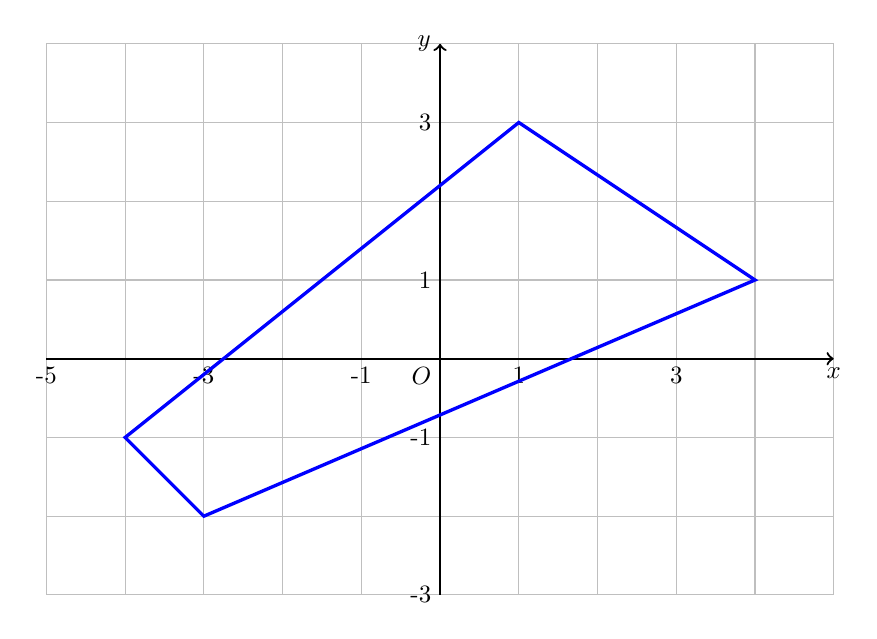
\begin{tikzpicture}[scale=1]
    % Vẽ lưới
    \draw [gray!50,thin] (-5,-3) grid (5,4);
    % Vẽ trục tọa độ
    \draw[->,thick] (-5,0) -- (5,0) node[below] {$x$};
    \draw[->,thick] (0,-3) -- (0,4) node[left] {$y$};
    
    % Đặt tên gốc O
    \node[below left] at (0,0) {$O$};
    
    % Đánh số trên trục x
    \foreach \x in {-5,-3,-1,1,3}
    \node[below] at (\x,0) {\x};
    
    % Đánh số trên trục y
    \foreach \y in {-3,-1,1,3}
    \node[left] at (0,\y) {\y};
    
    % Vẽ và tô miền đa giác
    %\filldraw[pattern=north east lines,pattern color=blue,draw=black,thick] 
    \draw[-, very thick, color=blue](-4,-1) -- (-3,-2) -- (4,1)-- (1,3) -- cycle;
    \end{tikzpicture}
\end{center}
\choice
{ $F(4;1)=18$ }
   { $F(-3;-2)=-9$ }
     { $F(0;0)=4$ }
    { \True $F(4;1)=14$ }
\loigiai{ 
 $F(-4;-1)=-14,F(-3;-2)=-8,F(4;1)=14,F(1;3)=-2$.

$F(4;1)=14$ là khẳng định đúng. 
 }\end{ex}

\begin{ex}
% ID: T10C2B4-162-TN
% Mức: VD
 Cho biểu thức $F=2 x + 3 y$ với $(x;y)$ là các điểm thuộc miền trong hình tứ giác như hình vẽ. Tìm khẳng định đúng. 
\begin{center}
 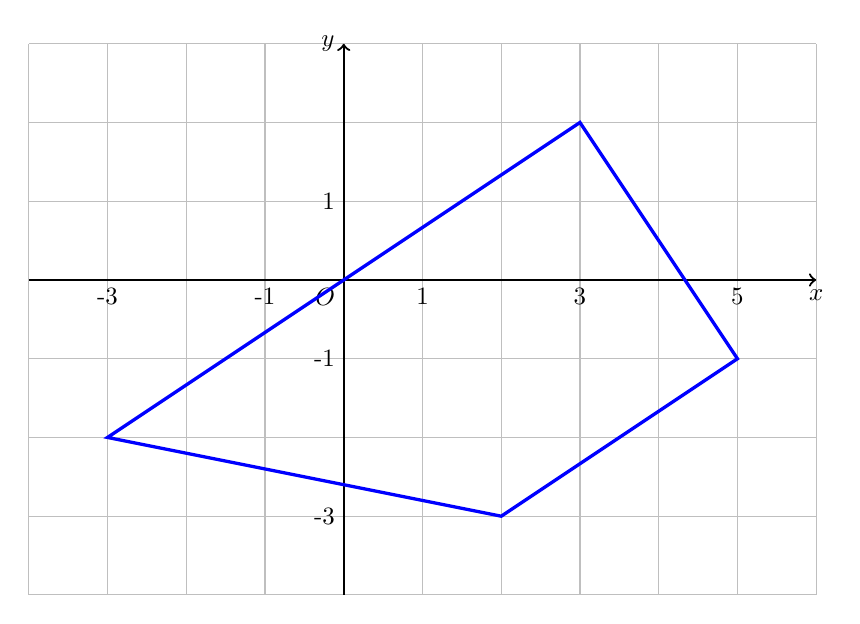
\begin{tikzpicture}[scale=1]
    % Vẽ lưới
    \draw [gray!50,thin] (-4,-4) grid (6,3);
    % Vẽ trục tọa độ
    \draw[->,thick] (-4,0) -- (6,0) node[below] {$x$};
    \draw[->,thick] (0,-4) -- (0,3) node[left] {$y$};
    
    % Đặt tên gốc O
    \node[below left] at (0,0) {$O$};
    
    % Đánh số trên trục x
    \foreach \x in {-3,-1,1,3,5}
    \node[below] at (\x,0) {\x};
    
    % Đánh số trên trục y
    \foreach \y in {-3,-1,1}
    \node[left] at (0,\y) {\y};
    
    % Vẽ và tô miền đa giác
    %\filldraw[pattern=north east lines,pattern color=blue,draw=black,thick] 
    \draw[-, very thick, color=blue](-3,-2) -- (2,-3) -- (5,-1)-- (3,2) -- cycle;
    \end{tikzpicture}
\end{center}
\choice
{ \True $F(-3;-2)=-12$ }
   { $F(5;-1)=12$ }
     { $F(2;-3)=-8$ }
    { $F(0;0)=-3$ }
\loigiai{ 
 $F(-3;-2)=-12,F(2;-3)=-5,F(5;-1)=7,F(3;2)=12$.

$F(-3;-2)=-12$ là khẳng định đúng. 
 }\end{ex}

\begin{ex}
% ID: T10C2B4-163-TN
% Mức: VD
 Cho biểu thức $F=4 x - y$ với $(x;y)$ là các điểm thuộc miền trong hình tứ giác như hình vẽ. Tìm khẳng định đúng. 
\begin{center}
 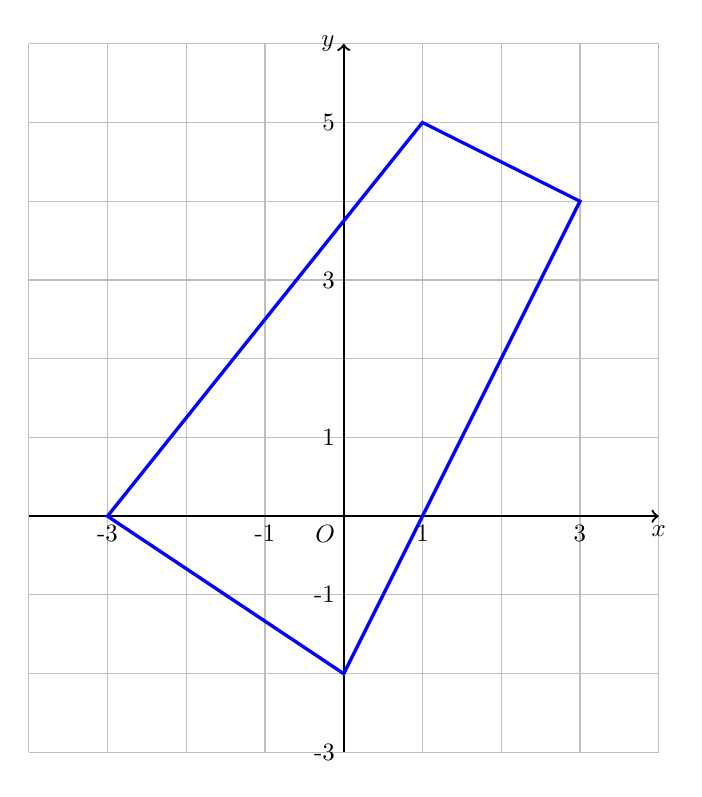
\begin{tikzpicture}[scale=1]
    % Vẽ lưới
    \draw [gray!50,thin] (-4,-3) grid (4,6);
    % Vẽ trục tọa độ
    \draw[->,thick] (-4,0) -- (4,0) node[below] {$x$};
    \draw[->,thick] (0,-3) -- (0,6) node[left] {$y$};
    
    % Đặt tên gốc O
    \node[below left] at (0,0) {$O$};
    
    % Đánh số trên trục x
    \foreach \x in {-3,-1,1,3}
    \node[below] at (\x,0) {\x};
    
    % Đánh số trên trục y
    \foreach \y in {-3,-1,1,3,5}
    \node[left] at (0,\y) {\y};
    
    % Vẽ và tô miền đa giác
    %\filldraw[pattern=north east lines,pattern color=blue,draw=black,thick] 
    \draw[-, very thick, color=blue](-3,0) -- (0,-2) -- (3,4)-- (1,5) -- cycle;
    \end{tikzpicture}
\end{center}
\choice
{ $F(0;0)=4$ }
   { \True $F(3;4)=8$ }
     { $F(1;5)=-5$ }
    { $F(0;-2)=0$ }
\loigiai{ 
 $F(-3;0)=-12,F(0;-2)=2,F(3;4)=8,F(1;5)=-1$.

$F(3;4)=8$ là khẳng định đúng. 
 }\end{ex}

\begin{ex}
% ID: T10C2B4-164-TN
% Mức: VD
 Cho biểu thức $F=3 x - y$ với $(x;y)$ là các điểm thuộc miền trong hình tứ giác như hình vẽ. Tìm khẳng định đúng. 
\begin{center}
 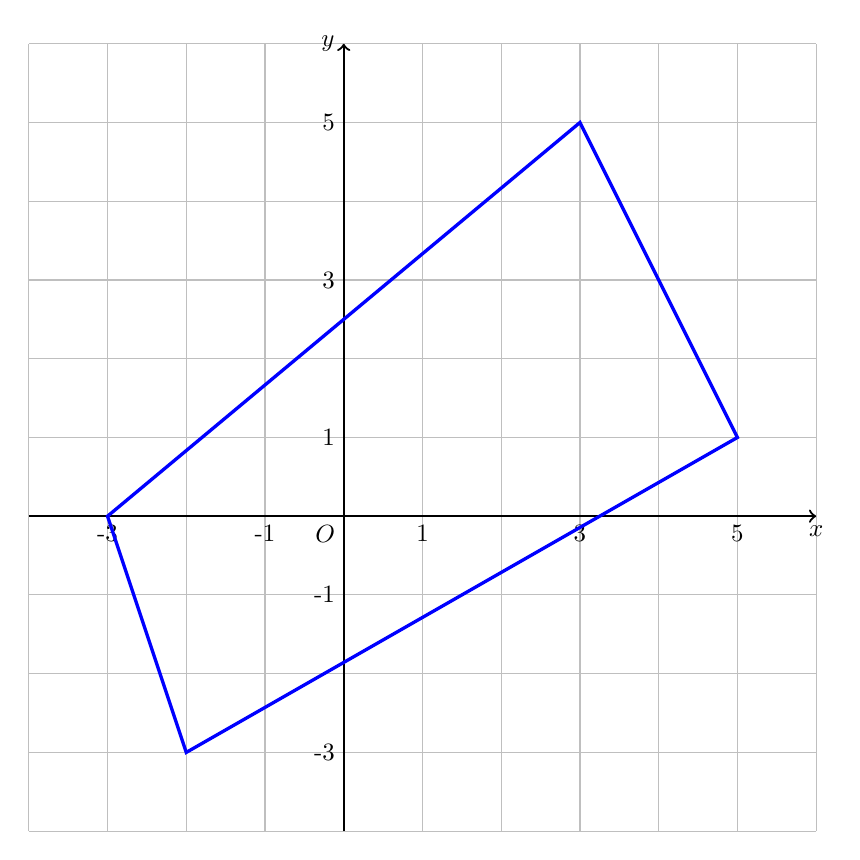
\begin{tikzpicture}[scale=1]
    % Vẽ lưới
    \draw [gray!50,thin] (-4,-4) grid (6,6);
    % Vẽ trục tọa độ
    \draw[->,thick] (-4,0) -- (6,0) node[below] {$x$};
    \draw[->,thick] (0,-4) -- (0,6) node[left] {$y$};
    
    % Đặt tên gốc O
    \node[below left] at (0,0) {$O$};
    
    % Đánh số trên trục x
    \foreach \x in {-3,-1,1,3,5}
    \node[below] at (\x,0) {\x};
    
    % Đánh số trên trục y
    \foreach \y in {-3,-1,1,3,5}
    \node[left] at (0,\y) {\y};
    
    % Vẽ và tô miền đa giác
    %\filldraw[pattern=north east lines,pattern color=blue,draw=black,thick] 
    \draw[-, very thick, color=blue](-3,0) -- (-2,-3) -- (5,1)-- (3,5) -- cycle;
    \end{tikzpicture}
\end{center}
\choice
{ $F(3;5)=2$ }
   { $F(5;1)=18$ }
     { \True $F(5;1)=14$ }
    { $F(-3;0)=-8$ }
\loigiai{ 
 $F(-3;0)=-9,F(-2;-3)=-3,F(5;1)=14,F(3;5)=4$.

$F(5;1)=14$ là khẳng định đúng. 
 }\end{ex}

\begin{ex}
% ID: T10C2B4-165-TN
% Mức: VD
 Cho biểu thức $F=2 x - y$ với $(x;y)$ là các điểm thuộc miền trong hình tứ giác như hình vẽ. Tìm khẳng định đúng. 
\begin{center}
 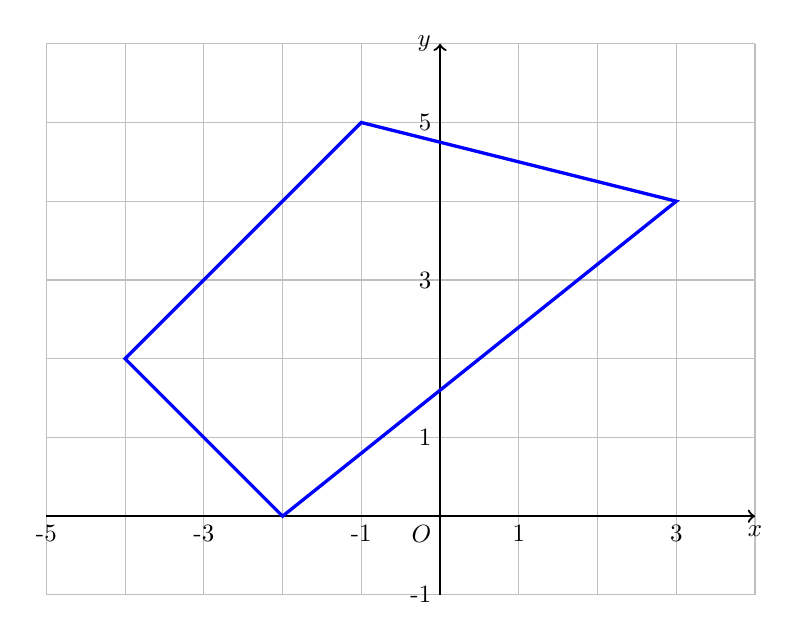
\begin{tikzpicture}[scale=1]
    % Vẽ lưới
    \draw [gray!50,thin] (-5,-1) grid (4,6);
    % Vẽ trục tọa độ
    \draw[->,thick] (-5,0) -- (4,0) node[below] {$x$};
    \draw[->,thick] (0,-1) -- (0,6) node[left] {$y$};
    
    % Đặt tên gốc O
    \node[below left] at (0,0) {$O$};
    
    % Đánh số trên trục x
    \foreach \x in {-5,-3,-1,1,3}
    \node[below] at (\x,0) {\x};
    
    % Đánh số trên trục y
    \foreach \y in {-1,1,3,5}
    \node[left] at (0,\y) {\y};
    
    % Vẽ và tô miền đa giác
    %\filldraw[pattern=north east lines,pattern color=blue,draw=black,thick] 
    \draw[-, very thick, color=blue](-4,2) -- (-2,0) -- (3,4)-- (-1,5) -- cycle;
    \end{tikzpicture}
\end{center}
\choice
{ $F(-1;5)=-10$ }
   { \True $F(-1;5)=-7$ }
     { $F(-4;2)=-9$ }
    { $F(3;4)=6$ }
\loigiai{ 
 $F(-4;2)=-10,F(-2;0)=-4,F(3;4)=2,F(-1;5)=-7$.

$F(-1;5)=-7$ là khẳng định đúng. 
 }\end{ex}

\begin{ex}
% ID: T10C2B4-166-TN
% Mức: VD
 Cho biểu thức $F=- 3 x - 5 y$ với $(x;y)$ là các điểm thuộc miền trong hình tứ giác như hình vẽ. Tìm khẳng định đúng. 
\begin{center}
 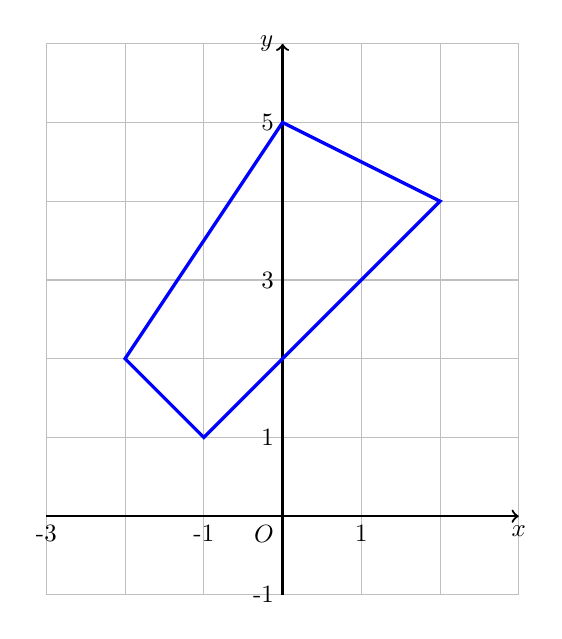
\begin{tikzpicture}[scale=1]
    % Vẽ lưới
    \draw [gray!50,thin] (-3,-1) grid (3,6);
    % Vẽ trục tọa độ
    \draw[->,thick] (-3,0) -- (3,0) node[below] {$x$};
    \draw[->,thick] (0,-1) -- (0,6) node[left] {$y$};
    
    % Đặt tên gốc O
    \node[below left] at (0,0) {$O$};
    
    % Đánh số trên trục x
    \foreach \x in {-3,-1,1}
    \node[below] at (\x,0) {\x};
    
    % Đánh số trên trục y
    \foreach \y in {-1,1,3,5}
    \node[left] at (0,\y) {\y};
    
    % Vẽ và tô miền đa giác
    %\filldraw[pattern=north east lines,pattern color=blue,draw=black,thick] 
    \draw[-, very thick, color=blue](-2,2) -- (-1,1) -- (2,4)-- (0,5) -- cycle;
    \end{tikzpicture}
\end{center}
\choice
{ \True $F(-2;2)=-4$ }
   { $F(0;5)=-30$ }
     { $F(-2;2)=-2$ }
    { $F(0;0)=-5$ }
\loigiai{ 
 $F(-2;2)=-4,F(-1;1)=-2,F(2;4)=-26,F(0;5)=-25$.

$F(-2;2)=-4$ là khẳng định đúng. 
 }\end{ex}

\begin{ex}
% ID: T10C2B4-167-TN
% Mức: VD
 Cho biểu thức $F=x + 5 y$ với $(x;y)$ là các điểm thuộc miền trong hình tứ giác như hình vẽ. Tìm khẳng định đúng. 
\begin{center}
 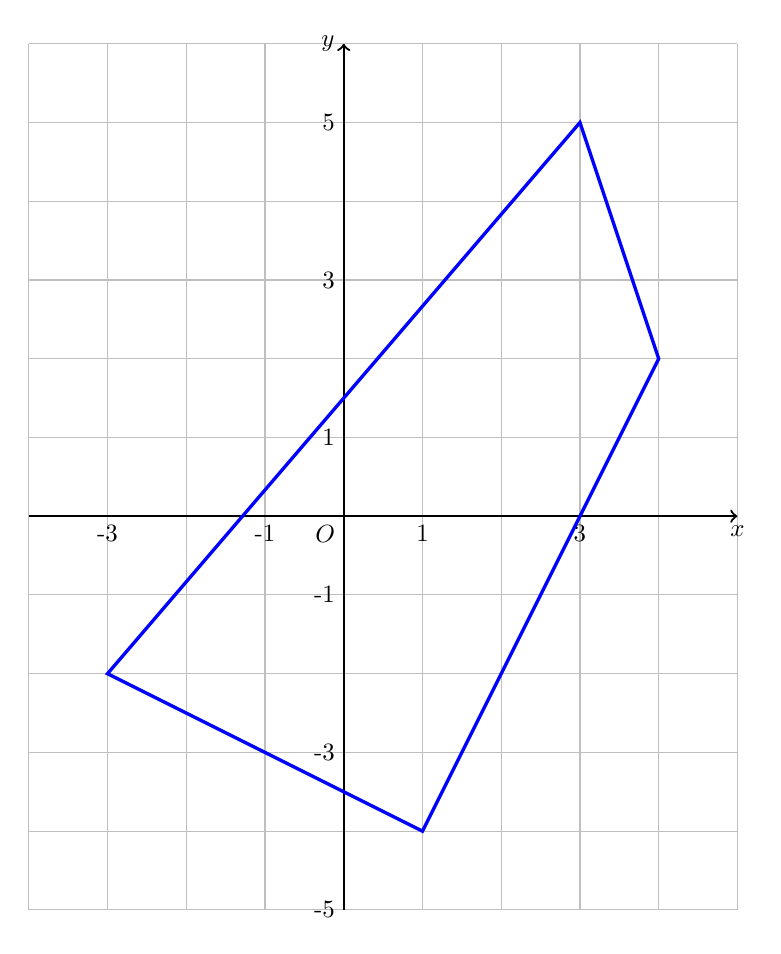
\begin{tikzpicture}[scale=1]
    % Vẽ lưới
    \draw [gray!50,thin] (-4,-5) grid (5,6);
    % Vẽ trục tọa độ
    \draw[->,thick] (-4,0) -- (5,0) node[below] {$x$};
    \draw[->,thick] (0,-5) -- (0,6) node[left] {$y$};
    
    % Đặt tên gốc O
    \node[below left] at (0,0) {$O$};
    
    % Đánh số trên trục x
    \foreach \x in {-3,-1,1,3}
    \node[below] at (\x,0) {\x};
    
    % Đánh số trên trục y
    \foreach \y in {-5,-3,-1,1,3,5}
    \node[left] at (0,\y) {\y};
    
    % Vẽ và tô miền đa giác
    %\filldraw[pattern=north east lines,pattern color=blue,draw=black,thick] 
    \draw[-, very thick, color=blue](-3,-2) -- (1,-4) -- (4,2)-- (3,5) -- cycle;
    \end{tikzpicture}
\end{center}
\choice
{ $F(0;0)=-4$ }
   { $F(-3;-2)=-11$ }
     { $F(1;-4)=-24$ }
    { \True $F(3;5)=28$ }
\loigiai{ 
 $F(-3;-2)=-13,F(1;-4)=-19,F(4;2)=14,F(3;5)=28$.

$F(3;5)=28$ là khẳng định đúng. 
 }\end{ex}

\begin{ex}
% ID: T10C2B4-168-TN
% Mức: VD
 Cho biểu thức $F=- 2 x + y$ với $(x;y)$ là các điểm thuộc miền trong hình tứ giác như hình vẽ. Tìm khẳng định đúng. 
\begin{center}
 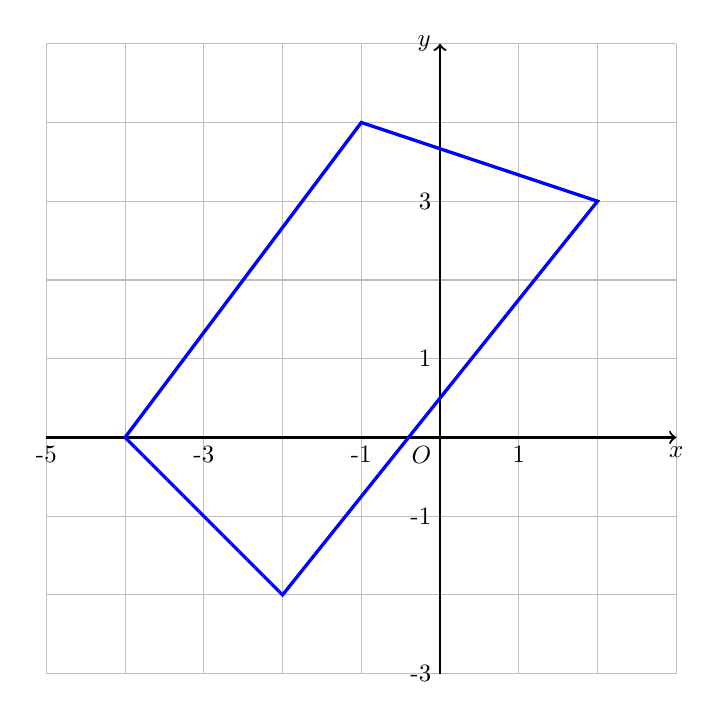
\begin{tikzpicture}[scale=1]
    % Vẽ lưới
    \draw [gray!50,thin] (-5,-3) grid (3,5);
    % Vẽ trục tọa độ
    \draw[->,thick] (-5,0) -- (3,0) node[below] {$x$};
    \draw[->,thick] (0,-3) -- (0,5) node[left] {$y$};
    
    % Đặt tên gốc O
    \node[below left] at (0,0) {$O$};
    
    % Đánh số trên trục x
    \foreach \x in {-5,-3,-1,1}
    \node[below] at (\x,0) {\x};
    
    % Đánh số trên trục y
    \foreach \y in {-3,-1,1,3}
    \node[left] at (0,\y) {\y};
    
    % Vẽ và tô miền đa giác
    %\filldraw[pattern=north east lines,pattern color=blue,draw=black,thick] 
    \draw[-, very thick, color=blue](-4,0) -- (-2,-2) -- (2,3)-- (-1,4) -- cycle;
    \end{tikzpicture}
\end{center}
\choice
{ \True $F(-4;0)=8$ }
   { $F(-4;0)=11$ }
     { $F(2;3)=2$ }
    { $F(-1;4)=1$ }
\loigiai{ 
 $F(-4;0)=8,F(-2;-2)=2,F(2;3)=-1,F(-1;4)=6$.

$F(-4;0)=8$ là khẳng định đúng. 
 }\end{ex}

\begin{ex}
% ID: T10C2B4-169-TN
% Mức: VD
 Cho biểu thức $F=x + 5 y$ với $(x;y)$ là các điểm thuộc miền trong hình tứ giác như hình vẽ. Tìm khẳng định đúng. 
\begin{center}
 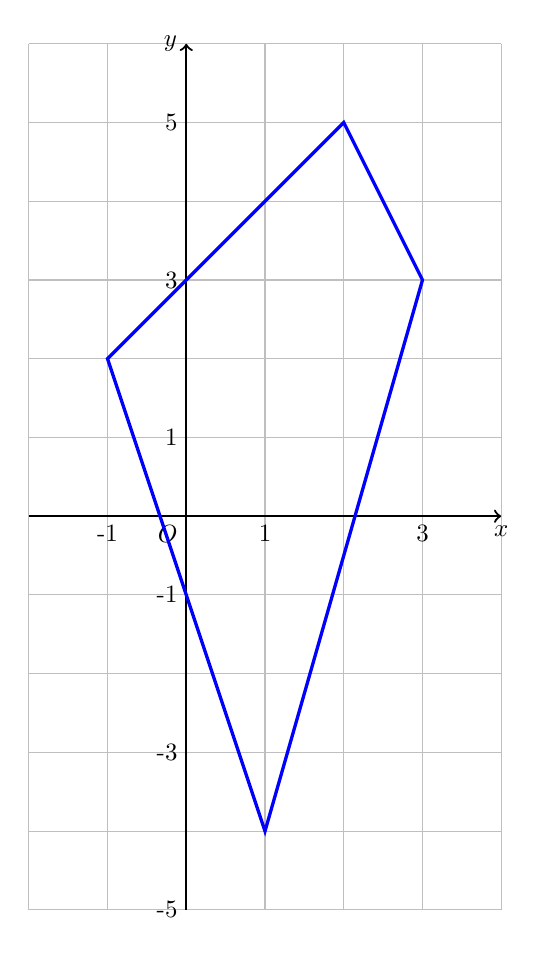
\begin{tikzpicture}[scale=1]
    % Vẽ lưới
    \draw [gray!50,thin] (-2,-5) grid (4,6);
    % Vẽ trục tọa độ
    \draw[->,thick] (-2,0) -- (4,0) node[below] {$x$};
    \draw[->,thick] (0,-5) -- (0,6) node[left] {$y$};
    
    % Đặt tên gốc O
    \node[below left] at (0,0) {$O$};
    
    % Đánh số trên trục x
    \foreach \x in {-1,1,3}
    \node[below] at (\x,0) {\x};
    
    % Đánh số trên trục y
    \foreach \y in {-5,-3,-1,1,3,5}
    \node[left] at (0,\y) {\y};
    
    % Vẽ và tô miền đa giác
    %\filldraw[pattern=north east lines,pattern color=blue,draw=black,thick] 
    \draw[-, very thick, color=blue](-1,2) -- (1,-4) -- (3,3)-- (2,5) -- cycle;
    \end{tikzpicture}
\end{center}
\choice
{ $F(2;5)=26$ }
   { $F(0;0)=-5$ }
     { \True $F(1;-4)=-19$ }
    { $F(-1;2)=12$ }
\loigiai{ 
 $F(-1;2)=9,F(1;-4)=-19,F(3;3)=18,F(2;5)=27$.

$F(1;-4)=-19$ là khẳng định đúng. 
 }\end{ex}

\begin{ex}
% ID: T10C2B4-170-TN
% Mức: VD
 Cho biểu thức $F=- 4 x - 2 y$ với $(x;y)$ là các điểm thuộc miền trong hình tứ giác như hình vẽ. Tìm khẳng định đúng. 
\begin{center}
 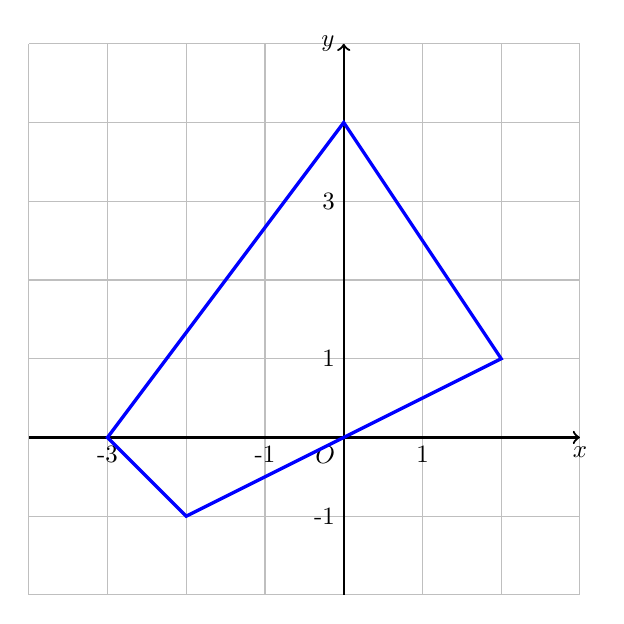
\begin{tikzpicture}[scale=1]
    % Vẽ lưới
    \draw [gray!50,thin] (-4,-2) grid (3,5);
    % Vẽ trục tọa độ
    \draw[->,thick] (-4,0) -- (3,0) node[below] {$x$};
    \draw[->,thick] (0,-2) -- (0,5) node[left] {$y$};
    
    % Đặt tên gốc O
    \node[below left] at (0,0) {$O$};
    
    % Đánh số trên trục x
    \foreach \x in {-3,-1,1}
    \node[below] at (\x,0) {\x};
    
    % Đánh số trên trục y
    \foreach \y in {-1,1,3}
    \node[left] at (0,\y) {\y};
    
    % Vẽ và tô miền đa giác
    %\filldraw[pattern=north east lines,pattern color=blue,draw=black,thick] 
    \draw[-, very thick, color=blue](-3,0) -- (-2,-1) -- (2,1)-- (0,4) -- cycle;
    \end{tikzpicture}
\end{center}
\choice
{ $F(-2;-1)=7$ }
   { $F(0;0)=-1$ }
     { \True $F(0;4)=-8$ }
    { $F(-3;0)=13$ }
\loigiai{ 
 $F(-3;0)=12,F(-2;-1)=10,F(2;1)=-10,F(0;4)=-8$.

$F(0;4)=-8$ là khẳng định đúng. 
 }\end{ex}



\dangbt{Kiểm tra cặp số là nghiệm của bất phương trình/hệ bất phương trình bậc nhất hai ẩn}
\begin{ex}
% ID: T10C2B4-171-TN
% Mức: TH
 Cặp số nào sau đây là nghiệm của hệ bất phương trình $\left\{ \begin{array}{l} 
    4 x + 5 y - 2 \ge 0\\ 
    x\le 8\\ 
    y \le 9
    \end{array} \right.$? 
\choice
{ \True $(4;6)$ }
   { (10, -8) }
     { (-3, 2) }
    { (17, 1) }
\loigiai{ 
 $(4;6)$ thỏa mãn hệ bất phương trình đã cho. 
 }\end{ex}

\begin{ex}
% ID: T10C2B4-172-TN
% Mức: TH
 Cặp số nào sau đây là nghiệm của hệ bất phương trình $\left\{ \begin{array}{l} 
    3 x + 5 y - 2 \ge 0\\ 
    x\le 6\\ 
    y \le 5
    \end{array} \right.$? 
\choice
{ (6, 16) }
   { (3, 10) }
     { (-9, 18) }
    { \True $(5;2)$ }
\loigiai{ 
 $(5;2)$ thỏa mãn hệ bất phương trình đã cho. 
 }\end{ex}

\begin{ex}
% ID: T10C2B4-173-TN
% Mức: TH
 Cặp số nào sau đây là nghiệm của hệ bất phương trình $\left\{ \begin{array}{l} 
    x + 2 y - 5 \ge 0\\ 
    x\le 13\\ 
    y \le 7
    \end{array} \right.$? 
\choice
{ (-6, -9) }
   { \True $(7;2)$ }
     { (17, -9) }
    { (13, 20) }
\loigiai{ 
 $(7;2)$ thỏa mãn hệ bất phương trình đã cho. 
 }\end{ex}

\begin{ex}
% ID: T10C2B4-174-TN
% Mức: TH
 Cặp số nào sau đây là nghiệm của hệ bất phương trình $\left\{ \begin{array}{l} 
    3 x + y - 5 \ge 0\\ 
    x\le 6\\ 
    y \le 14
    \end{array} \right.$? 
\choice
{ \True $(1;2)$ }
   { (20, 2) }
     { (14, -9) }
    { (7, -6) }
\loigiai{ 
 $(1;2)$ thỏa mãn hệ bất phương trình đã cho. 
 }\end{ex}

\begin{ex}
% ID: T10C2B4-175-TN
% Mức: TH
 Cặp số nào sau đây là nghiệm của hệ bất phương trình $\left\{ \begin{array}{l} 
    5 x + 2 y - 3 \ge 0\\ 
    x\le 8\\ 
    y \le 8
    \end{array} \right.$? 
\choice
{ (12, -9) }
   { \True $(5;5)$ }
     { (-5, 14) }
    { (1, 10) }
\loigiai{ 
 $(5;5)$ thỏa mãn hệ bất phương trình đã cho. 
 }\end{ex}

\begin{ex}
% ID: T10C2B4-176-TN
% Mức: TH
 Cặp số nào sau đây là nghiệm của hệ bất phương trình $\left\{ \begin{array}{l} 
    4 x + 4 y - 4 \ge 0\\ 
    x\le 8\\ 
    y \le 8
    \end{array} \right.$? 
\choice
{ (11, 15) }
   { \True $(2;6)$ }
     { (-4, -7) }
    { (8, 10) }
\loigiai{ 
 $(2;6)$ thỏa mãn hệ bất phương trình đã cho. 
 }\end{ex}

\begin{ex}
% ID: T10C2B4-177-TN
% Mức: TH
 Cặp số nào sau đây là nghiệm của hệ bất phương trình $\left\{ \begin{array}{l} 
    2 x + 5 y - 3 \ge 0\\ 
    x\le 10\\ 
    y \le 6
    \end{array} \right.$? 
\choice
{ (-8, 1) }
   { (5, -10) }
     { \True $(1;4)$ }
    { (14, 16) }
\loigiai{ 
 $(1;4)$ thỏa mãn hệ bất phương trình đã cho. 
 }\end{ex}

\begin{ex}
% ID: T10C2B4-178-TN
% Mức: TH
 Cặp số nào sau đây là nghiệm của hệ bất phương trình $\left\{ \begin{array}{l} 
    2 x + y - 4 \ge 0\\ 
    x\le 11\\ 
    y \le 13
    \end{array} \right.$? 
\choice
{ (15, 12) }
   { \True $(2;5)$ }
     { (20, 5) }
    { (-8, -8) }
\loigiai{ 
 $(2;5)$ thỏa mãn hệ bất phương trình đã cho. 
 }\end{ex}

\begin{ex}
% ID: T10C2B4-179-TN
% Mức: TH
 Cặp số nào sau đây là nghiệm của hệ bất phương trình $\left\{ \begin{array}{l} 
    2 x + 3 y - 6 \ge 0\\ 
    x\le 8\\ 
    y \le 7
    \end{array} \right.$? 
\choice
{ \True $(2;6)$ }
   { (14, -4) }
     { (-3, 10) }
    { (0, 14) }
\loigiai{ 
 $(2;6)$ thỏa mãn hệ bất phương trình đã cho. 
 }\end{ex}

\begin{ex}
% ID: T10C2B4-180-TN
% Mức: TH
 Cặp số nào sau đây là nghiệm của hệ bất phương trình $\left\{ \begin{array}{l} 
    x + 4 y - 4 \ge 0\\ 
    x\le 11\\ 
    y \le 8
    \end{array} \right.$? 
\choice
{ (-5, 5) }
   { (4, 11) }
     { \True $(1;2)$ }
    { (9, 13) }
\loigiai{ 
 $(1;2)$ thỏa mãn hệ bất phương trình đã cho. 
 }\end{ex}



\dangbt{Lập bất phương trình/hệ bất phương trình bậc nhất hai ẩn từ bài toán thực tế}
\begin{ex}
% ID: T10C2B4-181-TN
% Mức: VD
 Tính diện tích miền nghiệm của hệ bất phương trình sau

 $\left\{ \begin{array}{l} 
        2 x + 2 y - 24 \le 0\\ 
        x\ge 0\\ 
        y \ge 0
        \end{array} \right.$. 
\choice
{ ${24}$ }
   { \True ${72}$ }
     { ${288}$ }
    { ${144}$ }
\loigiai{ 
 Miền nghiệm của hệ bất phương trình là tam giác ${OAB}$ với $A(12;0), B(0;12)$.

 Diện tích tam giác ${OAB}$ là: $S=\frac{1}{2}.12.12=72$. 
 }\end{ex}

\begin{ex}
% ID: T10C2B4-182-TN
% Mức: VD
 Tính diện tích miền nghiệm của hệ bất phương trình sau

 $\left\{ \begin{array}{l} 
        - 3 x - y + 9 \ge 0\\ 
        x\ge 0\\ 
        y \ge 0
        \end{array} \right.$. 
\choice
{ \True ${\frac{27}{2}}$ }
   { ${12}$ }
     { ${54}$ }
    { ${27}$ }
\loigiai{ 
 Miền nghiệm của hệ bất phương trình là tam giác ${OAB}$ với $A(3;0), B(0;9)$.

 Diện tích tam giác ${OAB}$ là: $S=\frac{1}{2}.3.9=\frac{27}{2}$. 
 }\end{ex}

\begin{ex}
% ID: T10C2B4-183-TN
% Mức: VD
 Tính diện tích miền nghiệm của hệ bất phương trình sau

 $\left\{ \begin{array}{l} 
        - 3 x - y \ge -24\\ 
        x\ge 0\\ 
        y \ge 0
        \end{array} \right.$. 
\choice
{ ${384}$ }
   { ${38}$ }
     { ${192}$ }
    { \True ${96}$ }
\loigiai{ 
 Miền nghiệm của hệ bất phương trình là tam giác ${OAB}$ với $A(8;0), B(0;24)$.

 Diện tích tam giác ${OAB}$ là: $S=\frac{1}{2}.8.24=96$. 
 }\end{ex}

\begin{ex}
% ID: T10C2B4-184-TN
% Mức: VD
 Tính diện tích miền nghiệm của hệ bất phương trình sau

 $\left\{ \begin{array}{l} 
        x + y - 26 \le 0\\ 
        x\ge 0\\ 
        y \ge 0
        \end{array} \right.$. 
\choice
{ ${52}$ }
   { \True ${338}$ }
     { ${42}$ }
    { ${676}$ }
\loigiai{ 
 Miền nghiệm của hệ bất phương trình là tam giác ${OAB}$ với $A(26;0), B(0;26)$.

 Diện tích tam giác ${OAB}$ là: $S=\frac{1}{2}.26.26=338$. 
 }\end{ex}

\begin{ex}
% ID: T10C2B4-185-TN
% Mức: VD
 Tính diện tích miền nghiệm của hệ bất phương trình sau

 $\left\{ \begin{array}{l} 
        - x - y \ge -6\\ 
        x\ge 0\\ 
        y \ge 0
        \end{array} \right.$. 
\choice
{ ${36}$ }
   { ${19}$ }
     { ${12}$ }
    { \True ${18}$ }
\loigiai{ 
 Miền nghiệm của hệ bất phương trình là tam giác ${OAB}$ với $A(6;0), B(0;6)$.

 Diện tích tam giác ${OAB}$ là: $S=\frac{1}{2}.6.6=18$. 
 }\end{ex}

\begin{ex}
% ID: T10C2B4-186-TN
% Mức: VD
 Tính diện tích miền nghiệm của hệ bất phương trình sau

 $\left\{ \begin{array}{l} 
        - x - 3 y \ge -3\\ 
        x\ge 0\\ 
        y \ge 0
        \end{array} \right.$. 
\choice
{ ${4}$ }
   { ${6}$ }
     { \True ${\frac{3}{2}}$ }
    { ${23}$ }
\loigiai{ 
 Miền nghiệm của hệ bất phương trình là tam giác ${OAB}$ với $A(3;0), B(0;1)$.

 Diện tích tam giác ${OAB}$ là: $S=\frac{1}{2}.3.1=\frac{3}{2}$. 
 }\end{ex}

\begin{ex}
% ID: T10C2B4-187-TN
% Mức: VD
 Tính diện tích miền nghiệm của hệ bất phương trình sau

 $\left\{ \begin{array}{l} 
        4 x + 3 y - 24 \le 0\\ 
        x\ge 0\\ 
        y \ge 0
        \end{array} \right.$. 
\choice
{ ${60}$ }
   { ${14}$ }
     { \True ${24}$ }
    { ${48}$ }
\loigiai{ 
 Miền nghiệm của hệ bất phương trình là tam giác ${OAB}$ với $A(6;0), B(0;8)$.

 Diện tích tam giác ${OAB}$ là: $S=\frac{1}{2}.6.8=24$. 
 }\end{ex}

\begin{ex}
% ID: T10C2B4-188-TN
% Mức: VD
 Tính diện tích miền nghiệm của hệ bất phương trình sau

 $\left\{ \begin{array}{l} 
        x + y - 18 \le 0\\ 
        x\ge 0\\ 
        y \ge 0
        \end{array} \right.$. 
\choice
{ ${14}$ }
   { ${36}$ }
     { ${648}$ }
    { \True ${162}$ }
\loigiai{ 
 Miền nghiệm của hệ bất phương trình là tam giác ${OAB}$ với $A(18;0), B(0;18)$.

 Diện tích tam giác ${OAB}$ là: $S=\frac{1}{2}.18.18=162$. 
 }\end{ex}

\begin{ex}
% ID: T10C2B4-189-TN
% Mức: VD
 Tính diện tích miền nghiệm của hệ bất phương trình sau

 $\left\{ \begin{array}{l} 
        - 3 x - y \ge -18\\ 
        x\ge 0\\ 
        y \ge 0
        \end{array} \right.$. 
\choice
{ ${24}$ }
   { \True ${54}$ }
     { ${216}$ }
    { ${108}$ }
\loigiai{ 
 Miền nghiệm của hệ bất phương trình là tam giác ${OAB}$ với $A(6;0), B(0;18)$.

 Diện tích tam giác ${OAB}$ là: $S=\frac{1}{2}.6.18=54$. 
 }\end{ex}

\begin{ex}
% ID: T10C2B4-190-TN
% Mức: VD
 Tính diện tích miền nghiệm của hệ bất phương trình sau

 $\left\{ \begin{array}{l} 
        x + 2 y - 28 \le 0\\ 
        x\ge 0\\ 
        y \ge 0
        \end{array} \right.$. 
\choice
{ ${784}$ }
   { ${42}$ }
     { \True ${196}$ }
    { ${41}$ }
\loigiai{ 
 Miền nghiệm của hệ bất phương trình là tam giác ${OAB}$ với $A(28;0), B(0;14)$.

 Diện tích tam giác ${OAB}$ là: $S=\frac{1}{2}.28.14=196$. 
 }\end{ex}


\begin{ex}
% ID: T10C2B4-191-TN
% Mức: VD
Một học sinh rủ các bạn của mình đi xem phim, bạn đó dự tính chi tối đa 171 nghìn đồng cho việc mua bắp rang bơ và nước uống. Mỗi túi bắp rang bơ có giá 23 nghìn đồng và mỗi lon nước uống có giá 11 nghìn đồng. Nếu gọi ${x,y}$ lần lượt là số túi bắp rang bơ và số lon nước đã mua, hãy lập hệ bất phương trình biểu diễn đúng yêu cầu của bài toán, biết bạn đó đã mua cả bắp rang bơ và nước uống.
\choice
{$\begin{cases}x\in\mathbb{N};\ y\in\mathbb{N}\\11x+23y\le 171\end{cases}$}
{\True $\begin{cases}x\in\mathbb{N};\ y\in\mathbb{N}\\23x+11y\le 171\end{cases}$}
{$\begin{cases}x>0; y>0 \\11x+23y\le 171\end{cases}$}
{$\begin{cases}x\in\mathbb{N};\ y\in\mathbb{N}\\23x+11y\ge 171\end{cases}$}
\loigiai{
Do mua cả hai loại nên $x,y\in\mathbb{N}$.

Tổng số tiền phải trả là $23x+11y$ (nghìn đồng).

Vì số tiền chi tối đa là 171 nghìn đồng nên

$23x+11y\le 171$.

Vậy hệ điều kiện là
$\begin{cases}x\in\mathbb{N};\ y\in\mathbb{N}\\23x+11y\le 171\end{cases}$.
}
\end{ex}

\begin{ex}
% ID: T10C2B4-192-TN
% Mức: VD
Một học sinh rủ các bạn của mình đi xem phim, bạn đó dự tính chi tối đa 281 nghìn đồng cho việc mua bắp rang bơ và nước uống. Mỗi túi bắp rang bơ có giá 13 nghìn đồng và mỗi lon nước uống có giá 20 nghìn đồng. Nếu gọi ${x,y}$ lần lượt là số túi bắp rang bơ và số lon nước đã mua, hãy lập hệ bất phương trình biểu diễn đúng yêu cầu của bài toán, biết bạn đó đã mua cả bắp rang bơ và nước uống.
\choice
{$\begin{cases}x\in\mathbb{N};\ y\in\mathbb{N}\\13x+20y\ge 281\end{cases}$}
{\True $\begin{cases}x\in\mathbb{N};\ y\in\mathbb{N}\\13x+20y\le 281\end{cases}$}
{$\begin{cases}x\in\mathbb{N};\ y\in\mathbb{N}\\20x+13y\le 281\end{cases}$}
{$\begin{cases}x>0; y>0 \\20x+13y\le 281\end{cases}$}
\loigiai{
Do mua cả hai loại nên $x,y\in\mathbb{N}$.

Tổng số tiền phải trả là $13x+20y$ (nghìn đồng).

Vì số tiền chi tối đa là 281 nghìn đồng nên

$13x+20y\le 281$.

Vậy hệ điều kiện là
$\begin{cases}x\in\mathbb{N};\ y\in\mathbb{N}\\13x+20y\le 281\end{cases}$.
}
\end{ex}

\begin{ex}
% ID: T10C2B4-193-TN
% Mức: VD
Một học sinh rủ các bạn của mình đi xem phim, bạn đó dự tính chi tối đa 289 nghìn đồng cho việc mua bắp rang bơ và nước uống. Mỗi túi bắp rang bơ có giá 16 nghìn đồng và mỗi lon nước uống có giá 15 nghìn đồng. Nếu gọi ${x,y}$ lần lượt là số túi bắp rang bơ và số lon nước đã mua, hãy lập hệ bất phương trình biểu diễn đúng yêu cầu của bài toán, biết bạn đó đã mua cả bắp rang bơ và nước uống.
\choice
{$\begin{cases}x\in\mathbb{N};\ y\in\mathbb{N}\\15x+16y\le 289\end{cases}$}
{\True $\begin{cases}x\in\mathbb{N};\ y\in\mathbb{N}\\16x+15y\le 289\end{cases}$}
{$\begin{cases}x\in\mathbb{N};\ y\in\mathbb{N}\\16x+15y\ge 289\end{cases}$}
{$\begin{cases}x>0; y>0 \\15x+16y\le 289\end{cases}$}
\loigiai{
Do mua cả hai loại nên $x,y\in\mathbb{N}$.

Tổng số tiền phải trả là $16x+15y$ (nghìn đồng).

Vì số tiền chi tối đa là 289 nghìn đồng nên

$16x+15y\le 289$.

Vậy hệ điều kiện là
$\begin{cases}x\in\mathbb{N};\ y\in\mathbb{N}\\16x+15y\le 289\end{cases}$.
}
\end{ex}

\begin{ex}
% ID: T10C2B4-194-TN
% Mức: VD
Một học sinh rủ các bạn của mình đi xem phim, bạn đó dự tính chi tối đa 209 nghìn đồng cho việc mua bắp rang bơ và nước uống. Mỗi túi bắp rang bơ có giá 17 nghìn đồng và mỗi lon nước uống có giá 11 nghìn đồng. Nếu gọi ${x,y}$ lần lượt là số túi bắp rang bơ và số lon nước đã mua, hãy lập hệ bất phương trình biểu diễn đúng yêu cầu của bài toán, biết bạn đó đã mua cả bắp rang bơ và nước uống.
\choice
{\True $\begin{cases}x\in\mathbb{N};\ y\in\mathbb{N}\\17x+11y\le 209\end{cases}$}
{$\begin{cases}x\in\mathbb{N};\ y\in\mathbb{N}\\11x+17y\le 209\end{cases}$}
{$\begin{cases}x\in\mathbb{N};\ y\in\mathbb{N}\\17x+11y\ge 209\end{cases}$}
{$\begin{cases}x>0; y>0 \\11x+17y\le 209\end{cases}$}
\loigiai{
Do mua cả hai loại nên $x,y\in\mathbb{N}$.

Tổng số tiền phải trả là $17x+11y$ (nghìn đồng).

Vì số tiền chi tối đa là 209 nghìn đồng nên

$17x+11y\le 209$.

Vậy hệ điều kiện là
$\begin{cases}x\in\mathbb{N};\ y\in\mathbb{N}\\17x+11y\le 209\end{cases}$.
}
\end{ex}

\begin{ex}
% ID: T10C2B4-195-TN
% Mức: VD
Một học sinh rủ các bạn của mình đi xem phim, bạn đó dự tính chi tối đa 239 nghìn đồng cho việc mua bắp rang bơ và nước uống. Mỗi túi bắp rang bơ có giá 10 nghìn đồng và mỗi lon nước uống có giá 18 nghìn đồng. Nếu gọi ${x,y}$ lần lượt là số túi bắp rang bơ và số lon nước đã mua, hãy lập hệ bất phương trình biểu diễn đúng yêu cầu của bài toán, biết bạn đó đã mua cả bắp rang bơ và nước uống.
\choice
{$\begin{cases}x\in\mathbb{N};\ y\in\mathbb{N}\\18x+10y\le 239\end{cases}$}
{\True $\begin{cases}x\in\mathbb{N};\ y\in\mathbb{N}\\10x+18y\le 239\end{cases}$}
{$\begin{cases}x\in\mathbb{N};\ y\in\mathbb{N}\\10x+18y\ge 239\end{cases}$}
{$\begin{cases}x>0; y>0 \\18x+10y\le 239\end{cases}$}
\loigiai{
Do mua cả hai loại nên $x,y\in\mathbb{N}$.

Tổng số tiền phải trả là $10x+18y$ (nghìn đồng).

Vì số tiền chi tối đa là 239 nghìn đồng nên

$10x+18y\le 239$.

Vậy hệ điều kiện là
$\begin{cases}x\in\mathbb{N};\ y\in\mathbb{N}\\10x+18y\le 239\end{cases}$.
}
\end{ex}

\begin{ex}
% ID: T10C2B4-196-TN
% Mức: VD
Một học sinh rủ các bạn của mình đi xem phim, bạn đó dự tính chi tối đa 174 nghìn đồng cho việc mua bắp rang bơ và nước uống. Mỗi túi bắp rang bơ có giá 18 nghìn đồng và mỗi lon nước uống có giá 17 nghìn đồng. Nếu gọi ${x,y}$ lần lượt là số túi bắp rang bơ và số lon nước đã mua, hãy lập hệ bất phương trình biểu diễn đúng yêu cầu của bài toán, biết bạn đó đã mua cả bắp rang bơ và nước uống.
\choice
{$\begin{cases}x\in\mathbb{N};\ y\in\mathbb{N}\\17x+18y\le 174\end{cases}$}
{$\begin{cases}x>0; y>0 \\17x+18y\le 174\end{cases}$}
{\True $\begin{cases}x\in\mathbb{N};\ y\in\mathbb{N}\\18x+17y\le 174\end{cases}$}
{$\begin{cases}x\in\mathbb{N};\ y\in\mathbb{N}\\18x+17y\ge 174\end{cases}$}
\loigiai{
Do mua cả hai loại nên $x,y\in\mathbb{N}$.

Tổng số tiền phải trả là $18x+17y$ (nghìn đồng).

Vì số tiền chi tối đa là 174 nghìn đồng nên

$18x+17y\le 174$.

Vậy hệ điều kiện là
$\begin{cases}x\in\mathbb{N};\ y\in\mathbb{N}\\18x+17y\le 174\end{cases}$.
}
\end{ex}

\begin{ex}
% ID: T10C2B4-197-TN
% Mức: VD
Một học sinh rủ các bạn của mình đi xem phim, bạn đó dự tính chi tối đa 226 nghìn đồng cho việc mua bắp rang bơ và nước uống. Mỗi túi bắp rang bơ có giá 22 nghìn đồng và mỗi lon nước uống có giá 14 nghìn đồng. Nếu gọi ${x,y}$ lần lượt là số túi bắp rang bơ và số lon nước đã mua, hãy lập hệ bất phương trình biểu diễn đúng yêu cầu của bài toán, biết bạn đó đã mua cả bắp rang bơ và nước uống.
\choice
{$\begin{cases}x\in\mathbb{N};\ y\in\mathbb{N}\\14x+22y\le 226\end{cases}$}
{$\begin{cases}x\in\mathbb{N};\ y\in\mathbb{N}\\22x+14y\ge 226\end{cases}$}
{$\begin{cases}x>0; y>0 \\14x+22y\le 226\end{cases}$}
{\True $\begin{cases}x\in\mathbb{N};\ y\in\mathbb{N}\\22x+14y\le 226\end{cases}$}
\loigiai{
Do mua cả hai loại nên $x,y\in\mathbb{N}$.

Tổng số tiền phải trả là $22x+14y$ (nghìn đồng).

Vì số tiền chi tối đa là 226 nghìn đồng nên

$22x+14y\le 226$.

Vậy hệ điều kiện là
$\begin{cases}x\in\mathbb{N};\ y\in\mathbb{N}\\22x+14y\le 226\end{cases}$.
}
\end{ex}

\begin{ex}
% ID: T10C2B4-198-TN
% Mức: VD
Một học sinh rủ các bạn của mình đi xem phim, bạn đó dự tính chi tối đa 229 nghìn đồng cho việc mua bắp rang bơ và nước uống. Mỗi túi bắp rang bơ có giá 20 nghìn đồng và mỗi lon nước uống có giá 11 nghìn đồng. Nếu gọi ${x,y}$ lần lượt là số túi bắp rang bơ và số lon nước đã mua, hãy lập hệ bất phương trình biểu diễn đúng yêu cầu của bài toán, biết bạn đó đã mua cả bắp rang bơ và nước uống.
\choice
{$\begin{cases}x>0; y>0 \\11x+20y\le 229\end{cases}$}
{\True $\begin{cases}x\in\mathbb{N};\ y\in\mathbb{N}\\20x+11y\le 229\end{cases}$}
{$\begin{cases}x\in\mathbb{N};\ y\in\mathbb{N}\\11x+20y\le 229\end{cases}$}
{$\begin{cases}x\in\mathbb{N};\ y\in\mathbb{N}\\20x+11y\ge 229\end{cases}$}
\loigiai{
Do mua cả hai loại nên $x,y\in\mathbb{N}$.

Tổng số tiền phải trả là $20x+11y$ (nghìn đồng).

Vì số tiền chi tối đa là 229 nghìn đồng nên

$20x+11y\le 229$.

Vậy hệ điều kiện là
$\begin{cases}x\in\mathbb{N};\ y\in\mathbb{N}\\20x+11y\le 229\end{cases}$.
}
\end{ex}

\begin{ex}
% ID: T10C2B4-199-TN
% Mức: VD
Một học sinh rủ các bạn của mình đi xem phim, bạn đó dự tính chi tối đa 159 nghìn đồng cho việc mua bắp rang bơ và nước uống. Mỗi túi bắp rang bơ có giá 21 nghìn đồng và mỗi lon nước uống có giá 10 nghìn đồng. Nếu gọi ${x,y}$ lần lượt là số túi bắp rang bơ và số lon nước đã mua, hãy lập hệ bất phương trình biểu diễn đúng yêu cầu của bài toán, biết bạn đó đã mua cả bắp rang bơ và nước uống.
\choice
{$\begin{cases}x\in\mathbb{N};\ y\in\mathbb{N}\\21x+10y\ge 159\end{cases}$}
{\True $\begin{cases}x\in\mathbb{N};\ y\in\mathbb{N}\\21x+10y\le 159\end{cases}$}
{$\begin{cases}x\in\mathbb{N};\ y\in\mathbb{N}\\10x+21y\le 159\end{cases}$}
{$\begin{cases}x>0; y>0 \\10x+21y\le 159\end{cases}$}
\loigiai{
Do mua cả hai loại nên $x,y\in\mathbb{N}$.

Tổng số tiền phải trả là $21x+10y$ (nghìn đồng).

Vì số tiền chi tối đa là 159 nghìn đồng nên

$21x+10y\le 159$.

Vậy hệ điều kiện là
$\begin{cases}x\in\mathbb{N};\ y\in\mathbb{N}\\21x+10y\le 159\end{cases}$.
}
\end{ex}

\begin{ex}
% ID: T10C2B4-200-TN
% Mức: VD
Một học sinh rủ các bạn của mình đi xem phim, bạn đó dự tính chi tối đa 152 nghìn đồng cho việc mua bắp rang bơ và nước uống. Mỗi túi bắp rang bơ có giá 22 nghìn đồng và mỗi lon nước uống có giá 16 nghìn đồng. Nếu gọi ${x,y}$ lần lượt là số túi bắp rang bơ và số lon nước đã mua, hãy lập hệ bất phương trình biểu diễn đúng yêu cầu của bài toán, biết bạn đó đã mua cả bắp rang bơ và nước uống.
\choice
{$\begin{cases}x\in\mathbb{N};\ y\in\mathbb{N}\\22x+16y\ge 152\end{cases}$}
{$\begin{cases}x>0; y>0 \\16x+22y\le 152\end{cases}$}
{\True $\begin{cases}x\in\mathbb{N};\ y\in\mathbb{N}\\22x+16y\le 152\end{cases}$}
{$\begin{cases}x\in\mathbb{N};\ y\in\mathbb{N}\\16x+22y\le 152\end{cases}$}
\loigiai{
Do mua cả hai loại nên $x,y\in\mathbb{N}$.

Tổng số tiền phải trả là $22x+16y$ (nghìn đồng).

Vì số tiền chi tối đa là 152 nghìn đồng nên

$22x+16y\le 152$.

Vậy hệ điều kiện là
$\begin{cases}x\in\mathbb{N};\ y\in\mathbb{N}\\22x+16y\le 152\end{cases}$.
}
\end{ex}


\dangbt{Kiểm tra tính đúng sai của các khẳng định về bất phương trình/hệ bất phương trình bậc nhất hai ẩn và bài toán thực tế}
\begin{ex}
% ID: T10C2B4-201-TL
% Mức: TH
 Xét bất phương trình $- 3 x + 3 y - 3\ge 0$. Xét tính đúng-sai của các khẳng định sau. 
\choiceTFt
{ \True Cặp số $(1; 6)$ là một nghiệm của bất phương trình. }
   { Cặp số $(-6; -8)$ là nghiệm của bất phương trình  }
     { \True Miền nghiệm của bất phương trình chứa đường thẳng $d:- 3 x + 3 y - 3=0$ }
    { Miền nghiệm là nửa mặt phẳng không chứa điểm $(1; 6)$ và chứa đường thẳng $d:- 3 x + 3 y - 3=0$ }
\loigiai{ 
 

 a) Khẳng định đã cho là khẳng định đúng.

 Thay $(1; 6)$ vào bất phương trình thấy thỏa mãn nên $(1; 6)$ là một nghiệm của bất phương trình.

b) Khẳng định đã cho là khẳng định sai.

 Thay $(-6; -8)$ vào bất phương trình thấy không thỏa mãn nên $(-6; -8)$ không là nghiệm của bất phương trình.

c) Khẳng định đã cho là khẳng định đúng.

 Bất phương trình $- 3 x + 3 y - 3>0$ có miền nghiệm chứa đường thẳng $d:- 3 x + 3 y - 3=0$.

d) Khẳng định đã cho là khẳng định sai.

 Miền nghiệm là nửa mặt phẳng chứa điểm $(1; 6)$ và chứa đường thẳng $d:- 3 x + 3 y - 3=0$.

 
 }\end{ex}

\begin{ex}
% ID: T10C2B4-202-TL
% Mức: TH
 Xét bất phương trình $x + 2 y - 1<0$. Xét tính đúng-sai của các khẳng định sau. 
\choiceTFt
{ Cặp số $(5; -5)$ không là nghiệm của bất phương trình  }
   { Cặp số $(-6; 6)$ là nghiệm của bất phương trình  }
     { Miền nghiệm của bất phương trình chứa đường thẳng $d:x + 2 y - 1=0$ }
    { \True Miền nghiệm là nửa mặt phẳng chứa điểm $(-2;0)$ và không chứa đường thẳng $d:x + 2 y - 1=0$ }
\loigiai{ 
 

 a) Khẳng định đã cho là khẳng định sai.

 Thay $(5; -5)$ vào bất phương trình thấy thỏa mãn nên $(5; -5)$ là một nghiệm của bất phương trình.

b) Khẳng định đã cho là khẳng định sai.

 Thay $(-6; 6)$ vào bất phương trình thấy không thỏa mãn nên $(-6; 6)$ không là nghiệm của bất phương trình.

c) Khẳng định đã cho là khẳng định sai.

 Bất phương trình $x + 2 y - 1<0$ có miền nghiệm không chứa đường thẳng $x + 2 y - 1=0$.

d) Khẳng định đã cho là khẳng định đúng.

 Miền nghiệm là nửa mặt phẳng chứa điểm $(-2;0)$ và không chứa đường thẳng $d:x + 2 y - 1=0$.

 
 }\end{ex}

\begin{ex}
% ID: T10C2B4-203-TL
% Mức: TH
 Xét bất phương trình $- x + 3 y + 2<0$. Xét tính đúng-sai của các khẳng định sau. 
\choiceTFt
{ \True Cặp số $(4; -3)$ là một nghiệm của bất phương trình. }
   { \True Cặp số $(-8; -2)$ không là nghiệm của bất phương trình. }
     { Miền nghiệm của bất phương trình chứa đường thẳng $d:- x + 3 y + 2=0$ }
    { \True Miền nghiệm là nửa mặt phẳng chứa điểm $(2;-1)$ và không chứa đường thẳng $d:- x + 3 y + 2=0$ }
\loigiai{ 
 

 a) Khẳng định đã cho là khẳng định đúng.

 Thay $(4; -3)$ vào bất phương trình thấy thỏa mãn nên $(4; -3)$ là một nghiệm của bất phương trình.

b) Khẳng định đã cho là khẳng định đúng.

 Thay $(-8; -2)$ vào bất phương trình thấy không thỏa mãn nên $(-8; -2)$ không là nghiệm của bất phương trình.

c) Khẳng định đã cho là khẳng định sai.

 Bất phương trình $- x + 3 y + 2<0$ có miền nghiệm không chứa đường thẳng $- x + 3 y + 2=0$.

d) Khẳng định đã cho là khẳng định đúng.

 Miền nghiệm là nửa mặt phẳng chứa điểm $(2;-1)$ và không chứa đường thẳng $d:- x + 3 y + 2=0$.

 
 }\end{ex}

\begin{ex}
% ID: T10C2B4-204-TL
% Mức: TH
 Xét bất phương trình $- x + 2 y - 2<0$. Xét tính đúng-sai của các khẳng định sau. 
\choiceTFt
{ \True Cặp số $(8; 1)$ là một nghiệm của bất phương trình. }
   { \True Cặp số $(-5; 4)$ không là nghiệm của bất phương trình. }
     { \True Miền nghiệm của bất phương trình không chứa đường thẳng $d:- x + 2 y - 2=0$ }
    { Miền nghiệm là nửa mặt phẳng không chứa điểm $(-3;-2)$ và không chứa đường thẳng $d:- x + 2 y - 2=0$ }
\loigiai{ 
 

 a) Khẳng định đã cho là khẳng định đúng.

 Thay $(8; 1)$ vào bất phương trình thấy thỏa mãn nên $(8; 1)$ là một nghiệm của bất phương trình.

b) Khẳng định đã cho là khẳng định đúng.

 Thay $(-5; 4)$ vào bất phương trình thấy không thỏa mãn nên $(-5; 4)$ không là nghiệm của bất phương trình.

c) Khẳng định đã cho là khẳng định đúng.

 Bất phương trình $- x + 2 y - 2<0$ có miền nghiệm không chứa đường thẳng $- x + 2 y - 2=0$.

d) Khẳng định đã cho là khẳng định sai.

 Miền nghiệm là nửa mặt phẳng chứa điểm $(-3;-2)$ và không chứa đường thẳng $d:- x + 2 y - 2=0$.

 
 }\end{ex}

\begin{ex}
% ID: T10C2B4-205-TL
% Mức: TH
 Xét bất phương trình $- 2 x + y - 3>0$. Xét tính đúng-sai của các khẳng định sau. 
\choiceTFt
{ Cặp số $(-10; 6)$ không là nghiệm của bất phương trình  }
   { \True Cặp số $(-1; -2)$ không là nghiệm của bất phương trình. }
     { Miền nghiệm chứa đường thẳng $d:- 2 x + y - 3=0$ }
    { \True Miền nghiệm là nửa mặt phẳng chứa điểm $(-10; 6)$ và không chứa đường thẳng $d:- 2 x + y - 3=0$ }
\loigiai{ 
 

 a) Khẳng định đã cho là khẳng định sai.

 Thay $(-10; 6)$ vào bất phương trình thấy thỏa mãn nên $(-10; 6)$ là một nghiệm của bất phương trình.

b) Khẳng định đã cho là khẳng định đúng.

 Thay $(-1; -2)$ vào bất phương trình thấy không thỏa mãn nên $(-1; -2)$ không là nghiệm của bất phương trình.

c) Khẳng định đã cho là khẳng định sai.

 Bất phương trình $- 2 x + y - 3>0$ có miền nghiệm không chứa đường thẳng $- 2 x + y - 3=0$.

d) Khẳng định đã cho là khẳng định đúng.

 Miền nghiệm là nửa mặt phẳng chứa điểm $(-10; 6)$ và không chứa đường thẳng $d:- 2 x + y - 3=0$.

 
 }\end{ex}

\begin{ex}
% ID: T10C2B4-206-TL
% Mức: TH
 Xét bất phương trình $- x + 3 y + 1<0$. Xét tính đúng-sai của các khẳng định sau. 
\choiceTFt
{ Cặp số $(7; -9)$ không là nghiệm của bất phương trình  }
   { \True Cặp số $(-7; -1)$ không là nghiệm của bất phương trình. }
     { \True Miền nghiệm của bất phương trình không chứa đường thẳng $d:- x + 3 y + 1=0$ }
    { Miền nghiệm là nửa mặt phẳng chứa điểm $(-2;-3)$ và chứa đường thẳng $d:- x + 3 y + 1=0$ }
\loigiai{ 
 

 a) Khẳng định đã cho là khẳng định sai.

 Thay $(7; -9)$ vào bất phương trình thấy thỏa mãn nên $(7; -9)$ là một nghiệm của bất phương trình.

b) Khẳng định đã cho là khẳng định đúng.

 Thay $(-7; -1)$ vào bất phương trình thấy không thỏa mãn nên $(-7; -1)$ không là nghiệm của bất phương trình.

c) Khẳng định đã cho là khẳng định đúng.

 Bất phương trình $- x + 3 y + 1<0$ có miền nghiệm không chứa đường thẳng $- x + 3 y + 1=0$.

d) Khẳng định đã cho là khẳng định sai.

 Miền nghiệm là nửa mặt phẳng chứa điểm $(-2;-3)$ và không chứa đường thẳng $d:- x + 3 y + 1=0$.

 
 }\end{ex}

\begin{ex}
% ID: T10C2B4-207-TL
% Mức: TH
 Xét bất phương trình $x + 2 y + 2\ge 0$. Xét tính đúng-sai của các khẳng định sau. 
\choiceTFt
{ \True Cặp số $(9; -2)$ là một nghiệm của bất phương trình. }
   { Cặp số $(-8; -9)$ là nghiệm của bất phương trình  }
     { \True Miền nghiệm của bất phương trình chứa đường thẳng $d:x + 2 y + 2=0$ }
    { Miền nghiệm là nửa mặt phẳng không chứa điểm $(9; -2)$ và không chứa đường thẳng $d:x + 2 y + 2=0$ }
\loigiai{ 
 

 a) Khẳng định đã cho là khẳng định đúng.

 Thay $(9; -2)$ vào bất phương trình thấy thỏa mãn nên $(9; -2)$ là một nghiệm của bất phương trình.

b) Khẳng định đã cho là khẳng định sai.

 Thay $(-8; -9)$ vào bất phương trình thấy không thỏa mãn nên $(-8; -9)$ không là nghiệm của bất phương trình.

c) Khẳng định đã cho là khẳng định đúng.

 Bất phương trình $x + 2 y + 2>0$ có miền nghiệm chứa đường thẳng $d:x + 2 y + 2=0$.

d) Khẳng định đã cho là khẳng định sai.

 Miền nghiệm là nửa mặt phẳng chứa điểm $(9; -2)$ và chứa đường thẳng $d:x + 2 y + 2=0$.

 
 }\end{ex}

\begin{ex}
% ID: T10C2B4-208-TL
% Mức: TH
 Xét bất phương trình $2 x + 3 y + 1\ge 0$. Xét tính đúng-sai của các khẳng định sau. 
\choiceTFt
{ Cặp số $(9; -5)$ không là nghiệm của bất phương trình  }
   { \True Cặp số $(-3; -5)$ không là nghiệm của bất phương trình. }
     { \True Miền nghiệm của bất phương trình chứa đường thẳng $d:2 x + 3 y + 1=0$ }
    { \True Miền nghiệm là nửa mặt phẳng chứa điểm $(9; -5)$ và chứa đường thẳng $d:2 x + 3 y + 1=0$ }
\loigiai{ 
 

 a) Khẳng định đã cho là khẳng định sai.

 Thay $(9; -5)$ vào bất phương trình thấy thỏa mãn nên $(9; -5)$ là một nghiệm của bất phương trình.

b) Khẳng định đã cho là khẳng định đúng.

 Thay $(-3; -5)$ vào bất phương trình thấy không thỏa mãn nên $(-3; -5)$ không là nghiệm của bất phương trình.

c) Khẳng định đã cho là khẳng định đúng.

 Bất phương trình $2 x + 3 y + 1>0$ có miền nghiệm chứa đường thẳng $d:2 x + 3 y + 1=0$.

d) Khẳng định đã cho là khẳng định đúng.

 Miền nghiệm là nửa mặt phẳng chứa điểm $(9; -5)$ và chứa đường thẳng $d:2 x + 3 y + 1=0$.

 
 }\end{ex}

\begin{ex}
% ID: T10C2B4-209-TL
% Mức: TH
 Xét bất phương trình $x + 2 y + 3\le 0$. Xét tính đúng-sai của các khẳng định sau. 
\choiceTFt
{ \True Cặp số $(2;-3)$ là một nghiệm của bất phương trình. }
   { Cặp số $(-2;1)$ là nghiệm của bất phương trình  }
     { Miền nghiệm của bất phương trình khôngchứa đường thẳng $d:x + 2 y + 3=0$ }
    { Miền nghiệm là nửa mặt phẳng chứa điểm $(2;-3)$ và không chứa đường thẳng $d:x + 2 y + 3=0$ }
\loigiai{ 
 

 a) Khẳng định đã cho là khẳng định đúng.

 Thay $(2;-3)$ vào bất phương trình thấy thỏa mãn nên $(2;-3)$ là một nghiệm của bất phương trình.

b) Khẳng định đã cho là khẳng định sai.

 Thay $(-2;1)$ vào bất phương trình thấy không thỏa mãn nên $(-2;1)$ không là nghiệm của bất phương trình.

c) Khẳng định đã cho là khẳng định sai.

 Bất phương trình $x + 2 y + 3<0$ có miền nghiệm chứa đường thẳng $x + 2 y + 3=0$.

d) Khẳng định đã cho là khẳng định sai.

 Miền nghiệm là nửa mặt phẳng chứa điểm $(2;-3)$ và chứa đường thẳng $d:x + 2 y + 3=0$.

 
 }\end{ex}

\begin{ex}
% ID: T10C2B4-210-TL
% Mức: TH
 Xét bất phương trình $- 3 x + 3 y + 1\ge 0$. Xét tính đúng-sai của các khẳng định sau. 
\choiceTFt
{ \True Cặp số $(3; 5)$ là một nghiệm của bất phương trình. }
   { \True Cặp số $(8; 5)$ không là nghiệm của bất phương trình. }
     { \True Miền nghiệm của bất phương trình chứa đường thẳng $d:- 3 x + 3 y + 1=0$ }
    { \True Miền nghiệm là nửa mặt phẳng chứa điểm $(3; 5)$ và chứa đường thẳng $d:- 3 x + 3 y + 1=0$ }
\loigiai{ 
 

 a) Khẳng định đã cho là khẳng định đúng.

 Thay $(3; 5)$ vào bất phương trình thấy thỏa mãn nên $(3; 5)$ là một nghiệm của bất phương trình.

b) Khẳng định đã cho là khẳng định đúng.

 Thay $(8; 5)$ vào bất phương trình thấy không thỏa mãn nên $(8; 5)$ không là nghiệm của bất phương trình.

c) Khẳng định đã cho là khẳng định đúng.

 Bất phương trình $- 3 x + 3 y + 1>0$ có miền nghiệm chứa đường thẳng $d:- 3 x + 3 y + 1=0$.

d) Khẳng định đã cho là khẳng định đúng.

 Miền nghiệm là nửa mặt phẳng chứa điểm $(3; 5)$ và chứa đường thẳng $d:- 3 x + 3 y + 1=0$.

 
 }\end{ex}


\begin{ex}
% ID: T10C2B4-211-TL
% Mức: VD
 Bạn Nam thích ăn hai loại trái cây là táo và cam, mỗi tuần mẹ cho Nam 160000 đồng để mua trái cây. Biết rằng giá táo là 28000 đồng/1 kg, giá cam là 15000 đồng/1 kg. Gọi $x, y (x>0, y>0)$ lần lượt là số ki-lô-gam táo và cam mà Nam có thể mua về sử dụng trong một tuần.

 Xét tính đúng-sai của các khẳng định sau:
\choiceTFt
{ Trong tuần, số tiền mua táo là ${15000x}$ và số tiền mua cam là ${28000y}$ }
   { \True $28 x + 15 y\le 160 \, (1)$ }
     { \True  Cặp số (3;11) không là  nghiệm của bất phương trình $(1)$ }
    { \True  Bạn Nam không có thể mua 7 kg táo và 10 kg xoài }
\loigiai{ 
 

 a) Khẳng định đã cho là khẳng định sai.

 Số tiền mua táo là ${28000x}$ và số tiền mua cam là ${15000y}$.

b) Khẳng định đã cho là khẳng định đúng.

 Điều kiện: ${28000x}+{15000y} \le 160000 \Leftrightarrow 28 x + 15 y\le 160$.

c) Khẳng định đã cho là khẳng định đúng.

 $28.3+15.11>160$ nên cặp số (3;11) không là nghiệm của $(1)$.

d) Khẳng định đã cho là khẳng định đúng.

 $28.7+15.10> 160$ nên bạn Nam có thể mua 7 kg táo và 10 kg xoài.

 
 }\end{ex}

\begin{ex}
% ID: T10C2B4-212-TL
% Mức: VD
 Bạn Phương thích ăn hai loại trái cây là mận và táo, mỗi tuần mẹ cho Phương 150000 đồng để mua trái cây. Biết rằng giá mận là 30000 đồng/1 kg, giá táo là 19000 đồng/1 kg. Gọi $x, y (x>0, y>0)$ lần lượt là số ki-lô-gam mận và táo mà Phương có thể mua về sử dụng trong một tuần.

 Xét tính đúng-sai của các khẳng định sau:
\choiceTFt
{ \True Trong tuần, số tiền mua mận là ${30000x}$ và số tiền mua táo là ${19000y}$ }
   { $30 x + 19 y>150 \, (1)$ }
     { \True  Cặp số (2;2) là một nghiệm của bất phương trình $(1)$ }
    { Bạn Phương không thể mua 1 kg mận và 3 kg xoài }
\loigiai{ 
 

 a) Khẳng định đã cho là khẳng định đúng.

 Số tiền mua mận là ${30000x}$ và số tiền mua táo là ${19000y}$.

b) Khẳng định đã cho là khẳng định sai.

 Điều kiện: ${30000x}+{19000y} \le 150000 \Leftrightarrow 30 x + 19 y\le 150$.

c) Khẳng định đã cho là khẳng định đúng.

 $30.2+19.2\le 150$ nên cặp số (2;2) là một nghiệm của $(1)$.

d) Khẳng định đã cho là khẳng định sai.

 $30.1+19.3\le 150$ nên bạn Phương có thể mua 1 kg mận và 3 kg xoài.

 
 }\end{ex}

\begin{ex}
% ID: T10C2B4-213-TL
% Mức: VD
 Bạn Nam thích ăn hai loại trái cây là mận và xoài, mỗi tuần mẹ cho Nam 200000 đồng để mua trái cây. Biết rằng giá mận là 30000 đồng/1 kg, giá xoài là 18000 đồng/1 kg. Gọi $x, y (x>0, y>0)$ lần lượt là số ki-lô-gam mận và xoài mà Nam có thể mua về sử dụng trong một tuần.

 Xét tính đúng-sai của các khẳng định sau:
\choiceTFt
{ Trong tuần, số tiền mua mận là ${18000x}$ và số tiền mua xoài là ${30000y}$ }
   { \True $15 x + 9 y\le 100 \, (1)$ }
     { Cặp số (1;1) không là nghiệm của bất phương trình $(1)$ }
    { Bạn Nam có thể mua 6 kg mận và 5 kg xoài }
\loigiai{ 
 

 a) Khẳng định đã cho là khẳng định sai.

 Số tiền mua mận là ${30000x}$ và số tiền mua xoài là ${18000y}$.

b) Khẳng định đã cho là khẳng định đúng.

 Điều kiện: ${30000x}+{18000y} \le 200000 \Leftrightarrow 15 x + 9 y\le 100$.

c) Khẳng định đã cho là khẳng định sai.

 $15.1+9.1\le 100$ nên cặp số (1;1) là một nghiệm của $(1)$.

d) Khẳng định đã cho là khẳng định sai.

 $15.6+9.5> 100$ nên bạn Nam có thể mua 6 kg mận và 5 kg xoài.

 
 }\end{ex}

\begin{ex}
% ID: T10C2B4-214-TL
% Mức: VD
 Bạn Nam thích ăn hai loại trái cây là ổi và táo, mỗi tuần mẹ cho Nam 120000 đồng để mua trái cây. Biết rằng giá ổi là 34000 đồng/1 kg, giá táo là 23000 đồng/1 kg. Gọi $x, y (x>0, y>0)$ lần lượt là số ki-lô-gam ổi và táo mà Nam có thể mua về sử dụng trong một tuần.

 Xét tính đúng-sai của các khẳng định sau:
\choiceTFt
{ \True Trong tuần, số tiền mua ổi là ${34000x}$ và số tiền mua táo là ${23000y}$ }
   { \True $34 x + 23 y\le 120 \, (1)$ }
     { Cặp số (1;3) không là nghiệm của bất phương trình $(1)$ }
    { \True  Bạn Nam có thể mua 2 kg ổi và 2 kg xoài }
\loigiai{ 
 

 a) Khẳng định đã cho là khẳng định đúng.

 Số tiền mua ổi là ${34000x}$ và số tiền mua táo là ${23000y}$.

b) Khẳng định đã cho là khẳng định đúng.

 Điều kiện: ${34000x}+{23000y} \le 120000 \Leftrightarrow 34 x + 23 y\le 120$.

c) Khẳng định đã cho là khẳng định sai.

 $34.1+23.3\le 120$ nên cặp số (1;3) là một nghiệm của $(1)$.

d) Khẳng định đã cho là khẳng định đúng.

 $34.2+23.2\le 120$ nên bạn Nam có thể mua 2 kg ổi và 2 kg xoài.

 
 }\end{ex}

\begin{ex}
% ID: T10C2B4-215-TL
% Mức: VD
 Bạn Minh thích ăn hai loại trái cây là cam và ổi, mỗi tuần mẹ cho Minh 140000 đồng để mua trái cây. Biết rằng giá cam là 31000 đồng/1 kg, giá ổi là 25000 đồng/1 kg. Gọi $x, y (x>0, y>0)$ lần lượt là số ki-lô-gam cam và ổi mà Minh có thể mua về sử dụng trong một tuần.

 Xét tính đúng-sai của các khẳng định sau:
\choiceTFt
{ \True Trong tuần, số tiền mua cam là ${31000x}$ và số tiền mua ổi là ${25000y}$ }
   { $31 x + 25 y>140 \, (1)$ }
     { \True  Cặp số (2;1) là một nghiệm của bất phương trình $(1)$ }
    { Bạn Minh không thể mua 1 kg cam và 3 kg xoài }
\loigiai{ 
 

 a) Khẳng định đã cho là khẳng định đúng.

 Số tiền mua cam là ${31000x}$ và số tiền mua ổi là ${25000y}$.

b) Khẳng định đã cho là khẳng định sai.

 Điều kiện: ${31000x}+{25000y} \le 140000 \Leftrightarrow 31 x + 25 y\le 140$.

c) Khẳng định đã cho là khẳng định đúng.

 $31.2+25.1\le 140$ nên cặp số (2;1) là một nghiệm của $(1)$.

d) Khẳng định đã cho là khẳng định sai.

 $31.1+25.3\le 140$ nên bạn Minh có thể mua 1 kg cam và 3 kg xoài.

 
 }\end{ex}

\begin{ex}
% ID: T10C2B4-216-TL
% Mức: VD
 Bạn Minh thích ăn hai loại trái cây là mận và táo, mỗi tuần mẹ cho Minh 130000 đồng để mua trái cây. Biết rằng giá mận là 35000 đồng/1 kg, giá táo là 17000 đồng/1 kg. Gọi $x, y (x>0, y>0)$ lần lượt là số ki-lô-gam mận và táo mà Minh có thể mua về sử dụng trong một tuần.

 Xét tính đúng-sai của các khẳng định sau:
\choiceTFt
{ Trong tuần, số tiền mua mận là ${17000x}$ và số tiền mua táo là ${35000y}$ }
   { \True $35 x + 17 y\le 130 \, (1)$ }
     { Cặp số (1;2) không là nghiệm của bất phương trình $(1)$ }
    { Bạn Minh không thể mua 3 kg mận và 1 kg xoài }
\loigiai{ 
 

 a) Khẳng định đã cho là khẳng định sai.

 Số tiền mua mận là ${35000x}$ và số tiền mua táo là ${17000y}$.

b) Khẳng định đã cho là khẳng định đúng.

 Điều kiện: ${35000x}+{17000y} \le 130000 \Leftrightarrow 35 x + 17 y\le 130$.

c) Khẳng định đã cho là khẳng định sai.

 $35.1+17.2\le 130$ nên cặp số (1;2) là một nghiệm của $(1)$.

d) Khẳng định đã cho là khẳng định sai.

 $35.3+17.1\le 130$ nên bạn Minh có thể mua 3 kg mận và 1 kg xoài.

 
 }\end{ex}

\begin{ex}
% ID: T10C2B4-217-TL
% Mức: VD
 Bạn An thích ăn hai loại trái cây là mận và táo, mỗi tuần mẹ cho An 100000 đồng để mua trái cây. Biết rằng giá mận là 26000 đồng/1 kg, giá táo là 25000 đồng/1 kg. Gọi $x, y (x>0, y>0)$ lần lượt là số ki-lô-gam mận và táo mà An có thể mua về sử dụng trong một tuần.

 Xét tính đúng-sai của các khẳng định sau:
\choiceTFt
{ \True Trong tuần, số tiền mua mận là ${26000x}$ và số tiền mua táo là ${25000y}$ }
   { \True $26 x + 25 y\le 100 \, (1)$ }
     { \True  Cặp số (14;14) không là  nghiệm của bất phương trình $(1)$ }
    { Bạn An có thể mua 4 kg mận và 5 kg xoài }
\loigiai{ 
 

 a) Khẳng định đã cho là khẳng định đúng.

 Số tiền mua mận là ${26000x}$ và số tiền mua táo là ${25000y}$.

b) Khẳng định đã cho là khẳng định đúng.

 Điều kiện: ${26000x}+{25000y} \le 100000 \Leftrightarrow 26 x + 25 y\le 100$.

c) Khẳng định đã cho là khẳng định đúng.

 $26.14+25.14>100$ nên cặp số (14;14) không là nghiệm của $(1)$.

d) Khẳng định đã cho là khẳng định sai.

 $26.4+25.5> 100$ nên bạn An có thể mua 4 kg mận và 5 kg xoài.

 
 }\end{ex}

\begin{ex}
% ID: T10C2B4-218-TL
% Mức: VD
 Bạn An thích ăn hai loại trái cây là mận và cam, mỗi tuần mẹ cho An 110000 đồng để mua trái cây. Biết rằng giá mận là 33000 đồng/1 kg, giá cam là 22000 đồng/1 kg. Gọi $x, y (x>0, y>0)$ lần lượt là số ki-lô-gam mận và cam mà An có thể mua về sử dụng trong một tuần.

 Xét tính đúng-sai của các khẳng định sau:
\choiceTFt
{ Trong tuần, số tiền mua mận là ${22000x}$ và số tiền mua cam là ${33000y}$ }
   { $3 x + 2 y\ge 10 \, (1)$ }
     { Cặp số (1;5) là một nghiệm của bất phương trình $(1)$ }
    { \True  Bạn An không có thể mua 5 kg mận và 2 kg xoài }
\loigiai{ 
 

 a) Khẳng định đã cho là khẳng định sai.

 Số tiền mua mận là ${33000x}$ và số tiền mua cam là ${22000y}$.

b) Khẳng định đã cho là khẳng định sai.

 Điều kiện: ${33000x}+{22000y} \le 110000 \Leftrightarrow 3 x + 2 y\le 10$.

c) Khẳng định đã cho là khẳng định sai.

 $3.1+2.5>10$ nên cặp số (1;5) không là nghiệm của $(1)$.

d) Khẳng định đã cho là khẳng định đúng.

 $3.5+2.2> 10$ nên bạn An có thể mua 5 kg mận và 2 kg xoài.

 
 }\end{ex}

\begin{ex}
% ID: T10C2B4-219-TL
% Mức: VD
 Bạn Minh thích ăn hai loại trái cây là xoài và táo, mỗi tuần mẹ cho Minh 150000 đồng để mua trái cây. Biết rằng giá xoài là 35000 đồng/1 kg, giá táo là 20000 đồng/1 kg. Gọi $x, y (x>0, y>0)$ lần lượt là số ki-lô-gam xoài và táo mà Minh có thể mua về sử dụng trong một tuần.

 Xét tính đúng-sai của các khẳng định sau:
\choiceTFt
{ \True Trong tuần, số tiền mua xoài là ${35000x}$ và số tiền mua táo là ${20000y}$ }
   { \True $7 x + 4 y\le 30 \, (1)$ }
     { Cặp số (5;5) là một nghiệm của bất phương trình $(1)$ }
    { \True  Bạn Minh có thể mua 2 kg xoài và 3 kg xoài }
\loigiai{ 
 

 a) Khẳng định đã cho là khẳng định đúng.

 Số tiền mua xoài là ${35000x}$ và số tiền mua táo là ${20000y}$.

b) Khẳng định đã cho là khẳng định đúng.

 Điều kiện: ${35000x}+{20000y} \le 150000 \Leftrightarrow 7 x + 4 y\le 30$.

c) Khẳng định đã cho là khẳng định sai.

 $7.5+4.5>30$ nên cặp số (5;5) không là nghiệm của $(1)$.

d) Khẳng định đã cho là khẳng định đúng.

 $7.2+4.3\le 30$ nên bạn Minh có thể mua 2 kg xoài và 3 kg xoài.

 
 }\end{ex}

\begin{ex}
% ID: T10C2B4-220-TL
% Mức: VD
 Bạn Nga thích ăn hai loại trái cây là cam và mận, mỗi tuần mẹ cho Nga 180000 đồng để mua trái cây. Biết rằng giá cam là 34000 đồng/1 kg, giá mận là 15000 đồng/1 kg. Gọi $x, y (x>0, y>0)$ lần lượt là số ki-lô-gam cam và mận mà Nga có thể mua về sử dụng trong một tuần.

 Xét tính đúng-sai của các khẳng định sau:
\choiceTFt
{ Trong tuần, số tiền mua cam là ${15000x}$ và số tiền mua mận là ${34000y}$ }
   { $34 x + 15 y\ge 180 \, (1)$ }
     { \True  Cặp số (3;1) là một nghiệm của bất phương trình $(1)$ }
    { \True  Bạn Nga không có thể mua 7 kg cam và 9 kg xoài }
\loigiai{ 
 

 a) Khẳng định đã cho là khẳng định sai.

 Số tiền mua cam là ${34000x}$ và số tiền mua mận là ${15000y}$.

b) Khẳng định đã cho là khẳng định sai.

 Điều kiện: ${34000x}+{15000y} \le 180000 \Leftrightarrow 34 x + 15 y\le 180$.

c) Khẳng định đã cho là khẳng định đúng.

 $34.3+15.1\le 180$ nên cặp số (3;1) là một nghiệm của $(1)$.

d) Khẳng định đã cho là khẳng định đúng.

 $34.7+15.9> 180$ nên bạn Nga có thể mua 7 kg cam và 9 kg xoài.

 
 }\end{ex}


\begin{ex}
% ID: T10C2B4-221-TL
% Mức: TH
 Cho hệ bất phương trình $\left\{ \begin{array}{l}        2 x + y + 4 \ge 0\\         - 2 x + 2 y - 3 \ge 0        \end{array} \right.$. Xét tính đúng-sai của các khẳng định sau.
\choiceTFt
{ $(-3;4)$ không là một nghiệm của hệ bất phương trình }
   { $(0;-5)$ là một nghiệm của hệ bất phương trình  }
     { \True $(3;5)$ là một nghiệm của hệ bất phương trình }
    { $(4;4)$ là một nghiệm của hệ bất phương trình }
\loigiai{ 
 

 a) Khẳng định đã cho là khẳng định sai.

 Thay $(-3;4)$ vào thấy thỏa mãn nên $(-3;4)$ là một nghiệm của hệ bất phương trình.

b) Khẳng định đã cho là khẳng định sai.

 Thay $(0;-5)$ vào thấy không thỏa mãn nên $(0;-5)$ không là nghiệm của hệ bất phương trình.

c) Khẳng định đã cho là khẳng định đúng.

 Thay $(3;5)$  vào thấy thỏa mãn nên $(3;5)$ là một nghiệm của hệ bất phương trình.

d) Khẳng định đã cho là khẳng định sai.

 Thay $(4;4)$ vào thấy thỏa mãn nên $(4;4)$ là một nghiệm của hệ bất phương trình.

 
 }\end{ex}

\begin{ex}
% ID: T10C2B4-222-TL
% Mức: TH
 Cho hệ bất phương trình $\left\{ \begin{array}{l}        x + 3 y + 3 > 0\\         4 x - y + 1 \le 0        \end{array} \right.$. Xét tính đúng-sai của các khẳng định sau.
\choiceTFt
{ $(-5;2)$ không là một nghiệm của hệ bất phương trình }
   { \True $(-1;-1)$ không là nghiệm của hệ bất phương trình }
     { $(1;6)$ không là nghiệm của hệ bất phương trình }
    { $(5;19)$ là một nghiệm của hệ bất phương trình }
\loigiai{ 
 

 a) Khẳng định đã cho là khẳng định sai.

 Thay $(-5;2)$ vào thấy thỏa mãn nên $(-5;2)$ là một nghiệm của hệ bất phương trình.

b) Khẳng định đã cho là khẳng định đúng.

 Thay $(-1;-1)$ vào thấy không thỏa mãn nên $(-1;-1)$ không là nghiệm của hệ bất phương trình.

c) Khẳng định đã cho là khẳng định sai.

 Thay $(1;6)$  vào thấy thỏa mãn nên $(1;6)$ là một nghiệm của hệ bất phương trình.

d) Khẳng định đã cho là khẳng định sai.

 Thay $(5;19)$ vào thấy thỏa mãn nên $(5;19)$ là một nghiệm của hệ bất phương trình.

 
 }\end{ex}

\begin{ex}
% ID: T10C2B4-223-TL
% Mức: TH
 Cho hệ bất phương trình $\left\{ \begin{array}{l}        2 x + y + 3 \ge 0\\         - 3 x - 3 y - 1 \le 0        \end{array} \right.$. Xét tính đúng-sai của các khẳng định sau.
\choiceTFt
{ $(-5;10)$ không là một nghiệm của hệ bất phương trình }
   { \True $(0;-6)$ không là nghiệm của hệ bất phương trình }
     { $(3;-1)$ không là nghiệm của hệ bất phương trình }
    { $(6;-9)$ là một nghiệm của hệ bất phương trình }
\loigiai{ 
 

 a) Khẳng định đã cho là khẳng định sai.

 Thay $(-5;10)$ vào thấy thỏa mãn nên $(-5;10)$ là một nghiệm của hệ bất phương trình.

b) Khẳng định đã cho là khẳng định đúng.

 Thay $(0;-6)$ vào thấy không thỏa mãn nên $(0;-6)$ không là nghiệm của hệ bất phương trình.

c) Khẳng định đã cho là khẳng định sai.

 Thay $(3;-1)$  vào thấy thỏa mãn nên $(3;-1)$ là một nghiệm của hệ bất phương trình.

d) Khẳng định đã cho là khẳng định sai.

 Thay $(6;-9)$ vào thấy thỏa mãn nên $(6;-9)$ là một nghiệm của hệ bất phương trình.

 
 }\end{ex}

\begin{ex}
% ID: T10C2B4-224-TL
% Mức: TH
 Cho hệ bất phương trình $\left\{ \begin{array}{l}        x + y + 3 > 0\\         3 x - 2 y - 4 \le 0        \end{array} \right.$. Xét tính đúng-sai của các khẳng định sau.
\choiceTFt
{ $(-3;2)$ không là một nghiệm của hệ bất phương trình }
   { $(-2;-2)$ là một nghiệm của hệ bất phương trình  }
     { \True $(2;4)$ là một nghiệm của hệ bất phương trình }
    { \True $(4;2)$ không là nghiệm của hệ bất phương trình }
\loigiai{ 
 

 a) Khẳng định đã cho là khẳng định sai.

 Thay $(-3;2)$ vào thấy thỏa mãn nên $(-3;2)$ là một nghiệm của hệ bất phương trình.

b) Khẳng định đã cho là khẳng định sai.

 Thay $(-2;-2)$ vào thấy không thỏa mãn nên $(-2;-2)$ không là nghiệm của hệ bất phương trình.

c) Khẳng định đã cho là khẳng định đúng.

 Thay $(2;4)$  vào thấy thỏa mãn nên $(2;4)$ là một nghiệm của hệ bất phương trình.

d) Khẳng định đã cho là khẳng định đúng.

 Thay $(4;2)$ vào thấy thỏa mãn nên $(4;2)$ là một nghiệm của hệ bất phương trình.

 
 }\end{ex}

\begin{ex}
% ID: T10C2B4-225-TL
% Mức: TH
 Cho hệ bất phương trình $\left\{ \begin{array}{l}        3 x + 2 y - 1 \ge 0\\         - 2 x + 3 y - 4 \ge 0        \end{array} \right.$. Xét tính đúng-sai của các khẳng định sau.
\choiceTFt
{ $(-3;6)$ không là một nghiệm của hệ bất phương trình }
   { \True $(-1;1)$ không là nghiệm của hệ bất phương trình }
     { $(1;4)$ không là nghiệm của hệ bất phương trình }
    { $(6;4)$ là một nghiệm của hệ bất phương trình }
\loigiai{ 
 

 a) Khẳng định đã cho là khẳng định sai.

 Thay $(-3;6)$ vào thấy thỏa mãn nên $(-3;6)$ là một nghiệm của hệ bất phương trình.

b) Khẳng định đã cho là khẳng định đúng.

 Thay $(-1;1)$ vào thấy không thỏa mãn nên $(-1;1)$ không là nghiệm của hệ bất phương trình.

c) Khẳng định đã cho là khẳng định sai.

 Thay $(1;4)$  vào thấy thỏa mãn nên $(1;4)$ là một nghiệm của hệ bất phương trình.

d) Khẳng định đã cho là khẳng định sai.

 Thay $(6;4)$ vào thấy thỏa mãn nên $(6;4)$ là một nghiệm của hệ bất phương trình.

 
 }\end{ex}

\begin{ex}
% ID: T10C2B4-226-TL
% Mức: TH
 Cho hệ bất phương trình $\left\{ \begin{array}{l}        - 4 x + 2 y + 3 \ge 0\\         - 3 x - 3 y - 3 < 0        \end{array} \right.$. Xét tính đúng-sai của các khẳng định sau.
\choiceTFt
{ $(-3;5)$ không là một nghiệm của hệ bất phương trình }
   { \True $(-2;-7)$ không là nghiệm của hệ bất phương trình }
     { \True $(2;5)$ là một nghiệm của hệ bất phương trình }
    { $(5;-9)$ là một nghiệm của hệ bất phương trình }
\loigiai{ 
 

 a) Khẳng định đã cho là khẳng định sai.

 Thay $(-3;5)$ vào thấy thỏa mãn nên $(-3;5)$ là một nghiệm của hệ bất phương trình.

b) Khẳng định đã cho là khẳng định đúng.

 Thay $(-2;-7)$ vào thấy không thỏa mãn nên $(-2;-7)$ không là nghiệm của hệ bất phương trình.

c) Khẳng định đã cho là khẳng định đúng.

 Thay $(2;5)$  vào thấy thỏa mãn nên $(2;5)$ là một nghiệm của hệ bất phương trình.

d) Khẳng định đã cho là khẳng định sai.

 Thay $(5;-9)$ vào thấy thỏa mãn nên $(5;-9)$ là một nghiệm của hệ bất phương trình.

 
 }\end{ex}

\begin{ex}
% ID: T10C2B4-227-TL
% Mức: TH
 Cho hệ bất phương trình $\left\{ \begin{array}{l}        - x + 3 y + 4 > 0\\         - 2 x - y + 3 \le 0        \end{array} \right.$. Xét tính đúng-sai của các khẳng định sau.
\choiceTFt
{ \True $(-5;16)$ là một nghiệm của hệ bất phương trình }
   { \True $(0;-3)$ không là nghiệm của hệ bất phương trình }
     { $(2;1)$ không là nghiệm của hệ bất phương trình }
    { \True $(4;-8)$ không là nghiệm của hệ bất phương trình }
\loigiai{ 
 

 a) Khẳng định đã cho là khẳng định đúng.

 Thay $(-5;16)$ vào thấy thỏa mãn nên $(-5;16)$ là một nghiệm của hệ bất phương trình.

b) Khẳng định đã cho là khẳng định đúng.

 Thay $(0;-3)$ vào thấy không thỏa mãn nên $(0;-3)$ không là nghiệm của hệ bất phương trình.

c) Khẳng định đã cho là khẳng định sai.

 Thay $(2;1)$  vào thấy thỏa mãn nên $(2;1)$ là một nghiệm của hệ bất phương trình.

d) Khẳng định đã cho là khẳng định đúng.

 Thay $(4;-8)$ vào thấy thỏa mãn nên $(4;-8)$ là một nghiệm của hệ bất phương trình.

 
 }\end{ex}

\begin{ex}
% ID: T10C2B4-228-TL
% Mức: TH
 Cho hệ bất phương trình $\left\{ \begin{array}{l}        - 3 x + y - 1 \ge 0\\         x + 2 y - 4 \ge 0        \end{array} \right.$. Xét tính đúng-sai của các khẳng định sau.
\choiceTFt
{ \True $(-3;6)$ là một nghiệm của hệ bất phương trình }
   { \True $(-1;-3)$ không là nghiệm của hệ bất phương trình }
     { $(3;12)$ không là nghiệm của hệ bất phương trình }
    { $(5;-1)$ là một nghiệm của hệ bất phương trình }
\loigiai{ 
 

 a) Khẳng định đã cho là khẳng định đúng.

 Thay $(-3;6)$ vào thấy thỏa mãn nên $(-3;6)$ là một nghiệm của hệ bất phương trình.

b) Khẳng định đã cho là khẳng định đúng.

 Thay $(-1;-3)$ vào thấy không thỏa mãn nên $(-1;-3)$ không là nghiệm của hệ bất phương trình.

c) Khẳng định đã cho là khẳng định sai.

 Thay $(3;12)$  vào thấy thỏa mãn nên $(3;12)$ là một nghiệm của hệ bất phương trình.

d) Khẳng định đã cho là khẳng định sai.

 Thay $(5;-1)$ vào thấy thỏa mãn nên $(5;-1)$ là một nghiệm của hệ bất phương trình.

 
 }\end{ex}

\begin{ex}
% ID: T10C2B4-229-TL
% Mức: TH
 Cho hệ bất phương trình $\left\{ \begin{array}{l}        3 x + 2 y + 4 > 0\\         - 4 x + y + 2 > 0        \end{array} \right.$. Xét tính đúng-sai của các khẳng định sau.
\choiceTFt
{ $(-3;4)$ không là một nghiệm của hệ bất phương trình }
   { $(-1;-1)$ là một nghiệm của hệ bất phương trình  }
     { $(2;7)$ không là nghiệm của hệ bất phương trình }
    { $(5;17)$ là một nghiệm của hệ bất phương trình }
\loigiai{ 
 

 a) Khẳng định đã cho là khẳng định sai.

 Thay $(-3;4)$ vào thấy thỏa mãn nên $(-3;4)$ là một nghiệm của hệ bất phương trình.

b) Khẳng định đã cho là khẳng định sai.

 Thay $(-1;-1)$ vào thấy không thỏa mãn nên $(-1;-1)$ không là nghiệm của hệ bất phương trình.

c) Khẳng định đã cho là khẳng định sai.

 Thay $(2;7)$  vào thấy thỏa mãn nên $(2;7)$ là một nghiệm của hệ bất phương trình.

d) Khẳng định đã cho là khẳng định sai.

 Thay $(5;17)$ vào thấy thỏa mãn nên $(5;17)$ là một nghiệm của hệ bất phương trình.

 
 }\end{ex}

\begin{ex}
% ID: T10C2B4-230-TL
% Mức: TH
 Cho hệ bất phương trình $\left\{ \begin{array}{l}        - 3 x + 2 y - 1 \ge 0\\         x - 3 y - 3 \le 0        \end{array} \right.$. Xét tính đúng-sai của các khẳng định sau.
\choiceTFt
{ $(-4;-1)$ không là một nghiệm của hệ bất phương trình }
   { $(0;-3)$ là một nghiệm của hệ bất phương trình  }
     { $(1;3)$ không là nghiệm của hệ bất phương trình }
    { \True $(5;-3)$ không là nghiệm của hệ bất phương trình }
\loigiai{ 
 

 a) Khẳng định đã cho là khẳng định sai.

 Thay $(-4;-1)$ vào thấy thỏa mãn nên $(-4;-1)$ là một nghiệm của hệ bất phương trình.

b) Khẳng định đã cho là khẳng định sai.

 Thay $(0;-3)$ vào thấy không thỏa mãn nên $(0;-3)$ không là nghiệm của hệ bất phương trình.

c) Khẳng định đã cho là khẳng định sai.

 Thay $(1;3)$  vào thấy thỏa mãn nên $(1;3)$ là một nghiệm của hệ bất phương trình.

d) Khẳng định đã cho là khẳng định đúng.

 Thay $(5;-3)$ vào thấy thỏa mãn nên $(5;-3)$ là một nghiệm của hệ bất phương trình.

 
 }\end{ex}


\begin{ex}
% ID: T10C2B4-231-TL
% Mức: VDC
 Bác Sơn dự định trồng cà chua và dưa leo trên một mảnh đất có diện tích 6 sào. Nếu trồng 1 sào cà chua thì cần 3 ngày công và thu được 5 triệu đồng. Nếu trồng 1 sào dưa leo thì cần 6 ngày công và thu được 4 triệu đồng. Tổng số ngày công mà Bác Sơn có thể sử dụng không quá 24 ngày công. Gọi ${x, y}$ lần lượt là diện tích đất trồng cà chua và dưa leo (đơn vị: sào). Xét tính đúng-sai của các khẳng định sau:
\choiceTFt
{  Tổng diện tích đất cần dùng là $3x+6y$ }
   { \True $x+y \le 6$ }
     { $3x+6y \ge 24$ }
    { \True  Lợi nhuận lớn nhất thu được là 30 triệu đồng }
\loigiai{ 
 

 a) Khẳng định đã cho là khẳng định sai.

 Tổng diện tích đất cần dùng là $x+y$

b) Khẳng định đã cho là khẳng định đúng.

 $x+y \le 6$.

c) Khẳng định đã cho là khẳng định sai.

 $3x+6y \le 24$.

d) Khẳng định đã cho là khẳng định đúng.

 Gọi ${x,y}$ là diện tích đất để trồng cà chua và dưa leo.

$x\ge 0,y \ge 0$.

Diện tích đất cần dùng: $x+y \le 6$.

Số ngày công cần dùng: $3x+6y \le 24$.

Miền nghiệm của hệ điều kiện là tứ giác ${OABC}$với $O(0;0),A(0;4),B(4;2),C(6;0)$.

Lợi nhuận thu được: $F=5x+4y$.

$F(0;0)=0, F(0;4)=16, F(4;2)=28, F(6;0)=30$.

 Điểm thỏa mãn lợi nhuận lớn nhất:  $x = 6, y = 0$

 Lợi nhuận lớn nhất: F = 30 triệu đồng.

 
 }\end{ex}

\begin{ex}
% ID: T10C2B4-232-TL
% Mức: VDC
 Ông An dự định trồng lúa và khoai lang trên một mảnh đất có diện tích 10 sào. Nếu trồng 1 sào lúa thì cần 3 ngày công và thu được 5 triệu đồng. Nếu trồng 1 sào khoai lang thì cần 4 ngày công và thu được 7 triệu đồng. Tổng số ngày công mà Ông An có thể sử dụng không quá 36 ngày công. Gọi ${x, y}$ lần lượt là diện tích đất trồng lúa và khoai lang (đơn vị: sào). Xét tính đúng-sai của các khẳng định sau:
\choiceTFt
{  Tổng diện tích đất cần dùng là $3x+4y$ }
   { $x+y \ge 10$ }
     { $3x+4y \ge 36$ }
    { Lợi nhuận lớn nhất thu được là 64 triệu đồng }
\loigiai{ 
 

 a) Khẳng định đã cho là khẳng định sai.

 Tổng diện tích đất cần dùng là $x+y$

b) Khẳng định đã cho là khẳng định sai.

 $x+y \le 10$.

c) Khẳng định đã cho là khẳng định sai.

 $3x+4y \le 36$.

d) Khẳng định đã cho là khẳng định sai.

 Gọi ${x,y}$ là diện tích đất để trồng lúa và khoai lang.

$x\ge 0,y \ge 0$.

Diện tích đất cần dùng: $x+y \le 10$.

Số ngày công cần dùng: $3x+4y \le 36$.

Miền nghiệm của hệ điều kiện là tứ giác ${OABC}$với $O(0;0),A(0;9),B(4;6),C(10;0)$.

Lợi nhuận thu được: $F=5x+7y$.

$F(0;0)=0, F(0;9)=63, F(4;6)=62, F(10;0)=50$.

 Điểm thỏa mãn lợi nhuận lớn nhất:  $x = 0, y = 9$

 Lợi nhuận lớn nhất: F = 63 triệu đồng.

 
 }\end{ex}

\begin{ex}
% ID: T10C2B4-233-TL
% Mức: VDC
 Bác Nam dự định trồng cà chua và dưa leo trên một mảnh đất có diện tích 6 sào. Nếu trồng 1 sào cà chua thì cần 4 ngày công và thu được 8 triệu đồng. Nếu trồng 1 sào dưa leo thì cần 8 ngày công và thu được 7 triệu đồng. Tổng số ngày công mà Bác Nam có thể sử dụng không quá 40 ngày công. Gọi ${x, y}$ lần lượt là diện tích đất trồng cà chua và dưa leo (đơn vị: sào). Xét tính đúng-sai của các khẳng định sau:
\choiceTFt
{  Tổng diện tích đất cần dùng là $4x+8y$ }
   { $x+y \ge 6$ }
     { $4x+8y \ge 40$ }
    { Lợi nhuận lớn nhất thu được là 51 triệu đồng }
\loigiai{ 
 

 a) Khẳng định đã cho là khẳng định sai.

 Tổng diện tích đất cần dùng là $x+y$

b) Khẳng định đã cho là khẳng định sai.

 $x+y \le 6$.

c) Khẳng định đã cho là khẳng định sai.

 $4x+8y \le 40$.

d) Khẳng định đã cho là khẳng định sai.

 Gọi ${x,y}$ là diện tích đất để trồng cà chua và dưa leo.

$x\ge 0,y \ge 0$.

Diện tích đất cần dùng: $x+y \le 6$.

Số ngày công cần dùng: $4x+8y \le 40$.

Miền nghiệm của hệ điều kiện là tứ giác ${OABC}$với $O(0;0),A(0;5),B(2;4),C(6;0)$.

Lợi nhuận thu được: $F=8x+7y$.

$F(0;0)=0, F(0;5)=35, F(2;4)=44, F(6;0)=48$.

 Điểm thỏa mãn lợi nhuận lớn nhất:  $x = 6, y = 0$

 Lợi nhuận lớn nhất: F = 48 triệu đồng.

 
 }\end{ex}

\begin{ex}
% ID: T10C2B4-234-TL
% Mức: VDC
 Bác Sơn dự định trồng lúa và khoai lang trên một mảnh đất có diện tích 4 sào. Nếu trồng 1 sào lúa thì cần 3 ngày công và thu được 5 triệu đồng. Nếu trồng 1 sào khoai lang thì cần 8 ngày công và thu được 7 triệu đồng. Tổng số ngày công mà Bác Sơn có thể sử dụng không quá 24 ngày công. Gọi ${x, y}$ lần lượt là diện tích đất trồng lúa và khoai lang (đơn vị: sào). Xét tính đúng-sai của các khẳng định sau:
\choiceTFt
{  Tổng diện tích đất cần dùng là $3x+8y$ }
   { \True $x+y \le 4$ }
     { \True $3x+8y \le 24$ }
    { Lợi nhuận lớn nhất thu được là 29,8 triệu đồng }
\loigiai{ 
 

 a) Khẳng định đã cho là khẳng định sai.

 Tổng diện tích đất cần dùng là $x+y$

b) Khẳng định đã cho là khẳng định đúng.

 $x+y \le 4$.

c) Khẳng định đã cho là khẳng định đúng.

 $3x+8y \le 24$.

d) Khẳng định đã cho là khẳng định sai.

 Gọi ${x,y}$ là diện tích đất để trồng lúa và khoai lang.

$x\ge 0,y \ge 0$.

Diện tích đất cần dùng: $x+y \le 4$.

Số ngày công cần dùng: $3x+8y \le 24$.

Miền nghiệm của hệ điều kiện là tứ giác ${OABC}$với $O(0;0),A(0;3),B(\frac{8}{5};\frac{12}{5}),C(4;0)$.

Lợi nhuận thu được: $F=5x+7y$.

$F(0;0)=0, F(0;3)=21, F(\frac{8}{5};\frac{12}{5})=24, F(4;0)=20$.

 Điểm thỏa mãn lợi nhuận lớn nhất:  $x = \frac{8}{5}, y = \frac{12}{5}$

 Lợi nhuận lớn nhất: F = 24,8 triệu đồng.

 
 }\end{ex}

\begin{ex}
% ID: T10C2B4-235-TL
% Mức: VDC
 Bác Nam dự định trồng ngô và đậu xanh trên một mảnh đất có diện tích 10 sào. Nếu trồng 1 sào ngô thì cần 3 ngày công và thu được 3 triệu đồng. Nếu trồng 1 sào đậu xanh thì cần 4 ngày công và thu được 6 triệu đồng. Tổng số ngày công mà Bác Nam có thể sử dụng không quá 36 ngày công. Gọi ${x, y}$ lần lượt là diện tích đất trồng ngô và đậu xanh (đơn vị: sào). Xét tính đúng-sai của các khẳng định sau:
\choiceTFt
{ \True  Tổng diện tích đất cần dùng là $x+y$ }
   { \True $x+y \le 10$ }
     { $3x+4y \ge 36$ }
    { Lợi nhuận lớn nhất thu được là 56 triệu đồng }
\loigiai{ 
 

 a) Khẳng định đã cho là khẳng định đúng.

 Tổng diện tích đất cần dùng là $x+y$

b) Khẳng định đã cho là khẳng định đúng.

 $x+y \le 10$.

c) Khẳng định đã cho là khẳng định sai.

 $3x+4y \le 36$.

d) Khẳng định đã cho là khẳng định sai.

 Gọi ${x,y}$ là diện tích đất để trồng ngô và đậu xanh.

$x\ge 0,y \ge 0$.

Diện tích đất cần dùng: $x+y \le 10$.

Số ngày công cần dùng: $3x+4y \le 36$.

Miền nghiệm của hệ điều kiện là tứ giác ${OABC}$với $O(0;0),A(0;9),B(4;6),C(10;0)$.

Lợi nhuận thu được: $F=3x+6y$.

$F(0;0)=0, F(0;9)=54, F(4;6)=48, F(10;0)=30$.

 Điểm thỏa mãn lợi nhuận lớn nhất:  $x = 0, y = 9$

 Lợi nhuận lớn nhất: F = 54 triệu đồng.

 
 }\end{ex}

\begin{ex}
% ID: T10C2B4-236-TL
% Mức: VDC
 Bác Hùng dự định trồng ngô và đậu xanh trên một mảnh đất có diện tích 11 sào. Nếu trồng 1 sào ngô thì cần 3 ngày công và thu được 3 triệu đồng. Nếu trồng 1 sào đậu xanh thì cần 4 ngày công và thu được 5 triệu đồng. Tổng số ngày công mà Bác Hùng có thể sử dụng không quá 36 ngày công. Gọi ${x, y}$ lần lượt là diện tích đất trồng ngô và đậu xanh (đơn vị: sào). Xét tính đúng-sai của các khẳng định sau:
\choiceTFt
{ \True  Tổng diện tích đất cần dùng là $x+y$ }
   { \True $x+y \le 11$ }
     { $3x+4y \ge 36$ }
    { Lợi nhuận lớn nhất thu được là 46 triệu đồng }
\loigiai{ 
 

 a) Khẳng định đã cho là khẳng định đúng.

 Tổng diện tích đất cần dùng là $x+y$

b) Khẳng định đã cho là khẳng định đúng.

 $x+y \le 11$.

c) Khẳng định đã cho là khẳng định sai.

 $3x+4y \le 36$.

d) Khẳng định đã cho là khẳng định sai.

 Gọi ${x,y}$ là diện tích đất để trồng ngô và đậu xanh.

$x\ge 0,y \ge 0$.

Diện tích đất cần dùng: $x+y \le 11$.

Số ngày công cần dùng: $3x+4y \le 36$.

Miền nghiệm của hệ điều kiện là tứ giác ${OABC}$với $O(0;0),A(0;9),B(8;3),C(11;0)$.

Lợi nhuận thu được: $F=3x+5y$.

$F(0;0)=0, F(0;9)=45, F(8;3)=39, F(11;0)=33$.

 Điểm thỏa mãn lợi nhuận lớn nhất:  $x = 0, y = 9$

 Lợi nhuận lớn nhất: F = 45 triệu đồng.

 
 }\end{ex}

\begin{ex}
% ID: T10C2B4-237-TL
% Mức: VDC
 Chú Hải dự định trồng lúa và khoai lang trên một mảnh đất có diện tích 6 sào. Nếu trồng 1 sào lúa thì cần 4 ngày công và thu được 5 triệu đồng. Nếu trồng 1 sào khoai lang thì cần 8 ngày công và thu được 7 triệu đồng. Tổng số ngày công mà Chú Hải có thể sử dụng không quá 32 ngày công. Gọi ${x, y}$ lần lượt là diện tích đất trồng lúa và khoai lang (đơn vị: sào). Xét tính đúng-sai của các khẳng định sau:
\choiceTFt
{  Tổng diện tích đất cần dùng là $4x+8y$ }
   { $x+y \ge 6$ }
     { $4x+8y \ge 32$ }
    { \True  Lợi nhuận lớn nhất thu được là 34 triệu đồng }
\loigiai{ 
 

 a) Khẳng định đã cho là khẳng định sai.

 Tổng diện tích đất cần dùng là $x+y$

b) Khẳng định đã cho là khẳng định sai.

 $x+y \le 6$.

c) Khẳng định đã cho là khẳng định sai.

 $4x+8y \le 32$.

d) Khẳng định đã cho là khẳng định đúng.

 Gọi ${x,y}$ là diện tích đất để trồng lúa và khoai lang.

$x\ge 0,y \ge 0$.

Diện tích đất cần dùng: $x+y \le 6$.

Số ngày công cần dùng: $4x+8y \le 32$.

Miền nghiệm của hệ điều kiện là tứ giác ${OABC}$với $O(0;0),A(0;4),B(4;2),C(6;0)$.

Lợi nhuận thu được: $F=5x+7y$.

$F(0;0)=0, F(0;4)=28, F(4;2)=34, F(6;0)=30$.

 Điểm thỏa mãn lợi nhuận lớn nhất:  $x = 4, y = 2$

 Lợi nhuận lớn nhất: F = 34 triệu đồng.

 
 }\end{ex}

\begin{ex}
% ID: T10C2B4-238-TL
% Mức: VDC
 Bác Nam dự định trồng lúa và khoai lang trên một mảnh đất có diện tích 7 sào. Nếu trồng 1 sào lúa thì cần 4 ngày công và thu được 6 triệu đồng. Nếu trồng 1 sào khoai lang thì cần 8 ngày công và thu được 7 triệu đồng. Tổng số ngày công mà Bác Nam có thể sử dụng không quá 40 ngày công. Gọi ${x, y}$ lần lượt là diện tích đất trồng lúa và khoai lang (đơn vị: sào). Xét tính đúng-sai của các khẳng định sau:
\choiceTFt
{ \True  Tổng diện tích đất cần dùng là $x+y$ }
   { \True $x+y \le 7$ }
     { $4x+8y \ge 40$ }
    { \True  Lợi nhuận lớn nhất thu được là 45 triệu đồng }
\loigiai{ 
 

 a) Khẳng định đã cho là khẳng định đúng.

 Tổng diện tích đất cần dùng là $x+y$

b) Khẳng định đã cho là khẳng định đúng.

 $x+y \le 7$.

c) Khẳng định đã cho là khẳng định sai.

 $4x+8y \le 40$.

d) Khẳng định đã cho là khẳng định đúng.

 Gọi ${x,y}$ là diện tích đất để trồng lúa và khoai lang.

$x\ge 0,y \ge 0$.

Diện tích đất cần dùng: $x+y \le 7$.

Số ngày công cần dùng: $4x+8y \le 40$.

Miền nghiệm của hệ điều kiện là tứ giác ${OABC}$với $O(0;0),A(0;5),B(4;3),C(7;0)$.

Lợi nhuận thu được: $F=6x+7y$.

$F(0;0)=0, F(0;5)=35, F(4;3)=45, F(7;0)=42$.

 Điểm thỏa mãn lợi nhuận lớn nhất:  $x = 4, y = 3$

 Lợi nhuận lớn nhất: F = 45 triệu đồng.

 
 }\end{ex}

\begin{ex}
% ID: T10C2B4-239-TL
% Mức: VDC
 Chú Hải dự định trồng lúa và khoai lang trên một mảnh đất có diện tích 9 sào. Nếu trồng 1 sào lúa thì cần 4 ngày công và thu được 3 triệu đồng. Nếu trồng 1 sào khoai lang thì cần 8 ngày công và thu được 8 triệu đồng. Tổng số ngày công mà Chú Hải có thể sử dụng không quá 40 ngày công. Gọi ${x, y}$ lần lượt là diện tích đất trồng lúa và khoai lang (đơn vị: sào). Xét tính đúng-sai của các khẳng định sau:
\choiceTFt
{ \True  Tổng diện tích đất cần dùng là $x+y$ }
   { $x+y \ge 9$ }
     { \True $4x+8y \le 40$ }
    { \True  Lợi nhuận lớn nhất thu được là 40 triệu đồng }
\loigiai{ 
 

 a) Khẳng định đã cho là khẳng định đúng.

 Tổng diện tích đất cần dùng là $x+y$

b) Khẳng định đã cho là khẳng định sai.

 $x+y \le 9$.

c) Khẳng định đã cho là khẳng định đúng.

 $4x+8y \le 40$.

d) Khẳng định đã cho là khẳng định đúng.

 Gọi ${x,y}$ là diện tích đất để trồng lúa và khoai lang.

$x\ge 0,y \ge 0$.

Diện tích đất cần dùng: $x+y \le 9$.

Số ngày công cần dùng: $4x+8y \le 40$.

Miền nghiệm của hệ điều kiện là tứ giác ${OABC}$với $O(0;0),A(0;5),B(8;1),C(9;0)$.

Lợi nhuận thu được: $F=3x+8y$.

$F(0;0)=0, F(0;5)=40, F(8;1)=32, F(9;0)=27$.

 Điểm thỏa mãn lợi nhuận lớn nhất:  $x = 0, y = 5$

 Lợi nhuận lớn nhất: F = 40 triệu đồng.

 
 }\end{ex}

\begin{ex}
% ID: T10C2B4-240-TL
% Mức: VDC
 Bác Tín dự định trồng ngô và đậu xanh trên một mảnh đất có diện tích 8 sào. Nếu trồng 1 sào ngô thì cần 3 ngày công và thu được 3 triệu đồng. Nếu trồng 1 sào đậu xanh thì cần 6 ngày công và thu được 5 triệu đồng. Tổng số ngày công mà Bác Tín có thể sử dụng không quá 36 ngày công. Gọi ${x, y}$ lần lượt là diện tích đất trồng ngô và đậu xanh (đơn vị: sào). Xét tính đúng-sai của các khẳng định sau:
\choiceTFt
{  Tổng diện tích đất cần dùng là $3x+6y$ }
   { $x+y \ge 8$ }
     { \True $3x+6y \le 36$ }
    { \True  Lợi nhuận lớn nhất thu được là 32 triệu đồng }
\loigiai{ 
 

 a) Khẳng định đã cho là khẳng định sai.

 Tổng diện tích đất cần dùng là $x+y$

b) Khẳng định đã cho là khẳng định sai.

 $x+y \le 8$.

c) Khẳng định đã cho là khẳng định đúng.

 $3x+6y \le 36$.

d) Khẳng định đã cho là khẳng định đúng.

 Gọi ${x,y}$ là diện tích đất để trồng ngô và đậu xanh.

$x\ge 0,y \ge 0$.

Diện tích đất cần dùng: $x+y \le 8$.

Số ngày công cần dùng: $3x+6y \le 36$.

Miền nghiệm của hệ điều kiện là tứ giác ${OABC}$với $O(0;0),A(0;6),B(4;4),C(8;0)$.

Lợi nhuận thu được: $F=3x+5y$.

$F(0;0)=0, F(0;6)=30, F(4;4)=32, F(8;0)=24$.

 Điểm thỏa mãn lợi nhuận lớn nhất:  $x = 4, y = 4$

 Lợi nhuận lớn nhất: F = 32 triệu đồng.

 
 }\end{ex}


\begin{ex}
% ID: T10C2B4-241-TL
% Mức: VDC
 Bạn Lan dự định làm thủ công các bao lì xì để bán trong một hội chợ Tết. Cần 4 giờ để làm một bao lì xì đặc biệt có giá 21 nghìn đồng và 3 giờ để làm một bao lì xì thường có giá 13 nghìn đồng. Bạn Lan chỉ có 36 giờ để làm các bao lì xì và ban tổ chức hội chợ yêu cầu phải làm ít nhất 11 bao lì xì. Gọi ${x,y}$ lần lượt là số lượng bao lì xì đặc biệt và bao lì xì thường. Xét tính đúng-sai của các khẳng định sau. 
\choiceTFt
{  $x+y \le 11$ }
   {  $4x+3y \ge 36$ }
     { \True  Với $x = 3, y = 8$ thì số tiền thu về là lớn nhất }
    { Số tiền có thể thu về được nhiều nhất khi bán hết các bao lì xì là 176 ngàn đồng }
\loigiai{ 
 

 a) Khẳng định đã cho là khẳng định sai.

 $x+y \ge 11$.

b) Khẳng định đã cho là khẳng định sai.

 $4x+3y \le 36$.

c) Khẳng định đã cho là khẳng định đúng.

 Gọi ${x,y}$ là số lượng bao lì xì đặc biệt và bao lì xì thường.

$x\ge 0,y \ge 0$.

Số lượng bao lì xì cần làm: $x+y \ge 11$.

Số giờ cần dùng: $4x+3y \le 36$.

Miền nghiệm của hệ điều kiện là tam giác ${ABC}$ với $A(0;11),B(3;8),C(0;12)$.

$F (3, 8) = 167$

$F (0, 11) = 143$

$F (0, 12) = 156$



Lợi nhuận thu được: $F=21x+13y$.

Số tiền thu về lớn nhất khi:  $x = 3, y = 8$.

d) Khẳng định đã cho là khẳng định sai.

 Số tiền có thể thu về được nhiều nhất: F(3,8) = 167 ngàn đồng.

 
 }\end{ex}

\begin{ex}
% ID: T10C2B4-242-TL
% Mức: VDC
 Bạn Mai dự định làm thủ công các tấm thiệp để bán trong một hội chợ Tết. Cần 6 giờ để làm một tấm thiệp loại lớn có giá 18 nghìn đồng và 3 giờ để làm một tấm thiệp loại nhỏ có giá 13 nghìn đồng. Bạn Mai chỉ có 36 giờ để làm các tấm thiệp và ban tổ chức hội chợ yêu cầu phải làm ít nhất 11 tấm thiệp. Gọi ${x,y}$ lần lượt là số lượng tấm thiệp loại lớn và tấm thiệp loại nhỏ. Xét tính đúng-sai của các khẳng định sau. 
\choiceTFt
{ \True  $x+y \ge 11$ }
   { \True   $6x+3y \le 36$ }
     { Với $x = 2, y = 14$ thì số tiền thu về là lớn nhất }
    { \True  Số tiền có thể thu về được nhiều nhất khi bán hết các tấm thiệp là 156 ngàn đồng }
\loigiai{ 
 

 a) Khẳng định đã cho là khẳng định đúng.

 $x+y \ge 11$.

b) Khẳng định đã cho là khẳng định đúng.

 $6x+3y \le 36$.

c) Khẳng định đã cho là khẳng định sai.

 Gọi ${x,y}$ là số lượng tấm thiệp loại lớn và tấm thiệp loại nhỏ.

$x\ge 0,y \ge 0$.

Số lượng tấm thiệp cần làm: $x+y \ge 11$.

Số giờ cần dùng: $6x+3y \le 36$.

Miền nghiệm của hệ điều kiện là tam giác ${ABC}$ với $A(0;11),B(1;10),C(0;12)$.

$F (1, 10) = 148$

$F (0, 11) = 143$

$F (0, 12) = 156$



Lợi nhuận thu được: $F=18x+13y$.

Số tiền thu về lớn nhất khi:  $x = 0, y = 12$.

d) Khẳng định đã cho là khẳng định đúng.

 Số tiền có thể thu về được nhiều nhất: F(0,12) = 156 ngàn đồng.

 
 }\end{ex}

\begin{ex}
% ID: T10C2B4-243-TL
% Mức: VDC
 Bạn Phúc dự định làm thủ công các tấm thiệp để bán trong một hội chợ Tết. Cần 6 giờ để làm một tấm thiệp loại lớn có giá 19 nghìn đồng và 3 giờ để làm một tấm thiệp loại nhỏ có giá 10 nghìn đồng. Bạn Phúc chỉ có 36 giờ để làm các tấm thiệp và ban tổ chức hội chợ yêu cầu phải làm ít nhất 11 tấm thiệp. Gọi ${x,y}$ lần lượt là số lượng tấm thiệp loại lớn và tấm thiệp loại nhỏ. Xét tính đúng-sai của các khẳng định sau. 
\choiceTFt
{  $x+y \le 11$ }
   {  $6x+3y \ge 36$ }
     { \True  Với $x = 0, y = 12$ thì số tiền thu về là lớn nhất }
    { \True  Số tiền có thể thu về được nhiều nhất khi bán hết các tấm thiệp là 120 ngàn đồng }
\loigiai{ 
 

 a) Khẳng định đã cho là khẳng định sai.

 $x+y \ge 11$.

b) Khẳng định đã cho là khẳng định sai.

 $6x+3y \le 36$.

c) Khẳng định đã cho là khẳng định đúng.

 Gọi ${x,y}$ là số lượng tấm thiệp loại lớn và tấm thiệp loại nhỏ.

$x\ge 0,y \ge 0$.

Số lượng tấm thiệp cần làm: $x+y \ge 11$.

Số giờ cần dùng: $6x+3y \le 36$.

Miền nghiệm của hệ điều kiện là tam giác ${ABC}$ với $A(0;11),B(1;10),C(0;12)$.

$F (1, 10) = 119$

$F (0, 11) = 110$

$F (0, 12) = 120$



Lợi nhuận thu được: $F=19x+10y$.

Số tiền thu về lớn nhất khi:  $x = 0, y = 12$.

d) Khẳng định đã cho là khẳng định đúng.

 Số tiền có thể thu về được nhiều nhất: F(0,12) = 120 ngàn đồng.

 
 }\end{ex}

\begin{ex}
% ID: T10C2B4-244-TL
% Mức: VDC
 Bạn Khôi dự định làm thủ công các bao lì xì để bán trong một hội chợ Tết. Cần 4 giờ để làm một bao lì xì đặc biệt có giá 14 nghìn đồng và 3 giờ để làm một bao lì xì thường có giá 9 nghìn đồng. Bạn Khôi chỉ có 36 giờ để làm các bao lì xì và ban tổ chức hội chợ yêu cầu phải làm ít nhất 10 bao lì xì. Gọi ${x,y}$ lần lượt là số lượng bao lì xì đặc biệt và bao lì xì thường. Xét tính đúng-sai của các khẳng định sau. 
\choiceTFt
{ \True  $x+y \ge 10$ }
   { \True   $4x+3y \le 36$ }
     { \True  Với $x = 6, y = 4$ thì số tiền thu về là lớn nhất }
    { \True  Số tiền có thể thu về được nhiều nhất khi bán hết các bao lì xì là 120 ngàn đồng }
\loigiai{ 
 

 a) Khẳng định đã cho là khẳng định đúng.

 $x+y \ge 10$.

b) Khẳng định đã cho là khẳng định đúng.

 $4x+3y \le 36$.

c) Khẳng định đã cho là khẳng định đúng.

 Gọi ${x,y}$ là số lượng bao lì xì đặc biệt và bao lì xì thường.

$x\ge 0,y \ge 0$.

Số lượng bao lì xì cần làm: $x+y \ge 10$.

Số giờ cần dùng: $4x+3y \le 36$.

Miền nghiệm của hệ điều kiện là tam giác ${ABC}$ với $A(0;10),B(6;4),C(0;12)$.

$F (6, 4) = 120$

$F (0, 10) = 90$

$F (0, 12) = 108$



Lợi nhuận thu được: $F=14x+9y$.

Số tiền thu về lớn nhất khi:  $x = 6, y = 4$.

d) Khẳng định đã cho là khẳng định đúng.

 Số tiền có thể thu về được nhiều nhất: F(6,4) = 120 ngàn đồng.

 
 }\end{ex}

\begin{ex}
% ID: T10C2B4-245-TL
% Mức: VDC
 Bạn Phúc dự định làm thủ công các dây trang trí để bán trong một hội chợ Tết. Cần 6 giờ để làm một dây loại cầu kỳ có giá 22 nghìn đồng và 3 giờ để làm một dây loại đơn giản có giá 8 nghìn đồng. Bạn Phúc chỉ có 36 giờ để làm các dây trang trí và ban tổ chức hội chợ yêu cầu phải làm ít nhất 11 dây trang trí. Gọi ${x,y}$ lần lượt là số lượng dây loại cầu kỳ và dây loại đơn giản. Xét tính đúng-sai của các khẳng định sau. 
\choiceTFt
{ \True  $x+y \ge 11$ }
   { \True   $6x+3y \le 36$ }
     { Với $x = 3, y = 11$ thì số tiền thu về là lớn nhất }
    { Số tiền có thể thu về được nhiều nhất khi bán hết các dây trang trí là 108 ngàn đồng }
\loigiai{ 
 

 a) Khẳng định đã cho là khẳng định đúng.

 $x+y \ge 11$.

b) Khẳng định đã cho là khẳng định đúng.

 $6x+3y \le 36$.

c) Khẳng định đã cho là khẳng định sai.

 Gọi ${x,y}$ là số lượng dây loại cầu kỳ và dây loại đơn giản.

$x\ge 0,y \ge 0$.

Số lượng dây trang trí cần làm: $x+y \ge 11$.

Số giờ cần dùng: $6x+3y \le 36$.

Miền nghiệm của hệ điều kiện là tam giác ${ABC}$ với $A(0;11),B(1;10),C(0;12)$.

$F (1, 10) = 102$

$F (0, 11) = 88$

$F (0, 12) = 96$



Lợi nhuận thu được: $F=22x+8y$.

Số tiền thu về lớn nhất khi:  $x = 1, y = 10$.

d) Khẳng định đã cho là khẳng định sai.

 Số tiền có thể thu về được nhiều nhất: F(1,10) = 102 ngàn đồng.

 
 }\end{ex}

\begin{ex}
% ID: T10C2B4-246-TL
% Mức: VDC
 Bạn Mai dự định làm thủ công các dây trang trí để bán trong một hội chợ Tết. Cần 6 giờ để làm một dây loại cầu kỳ có giá 17 nghìn đồng và 3 giờ để làm một dây loại đơn giản có giá 10 nghìn đồng. Bạn Mai chỉ có 36 giờ để làm các dây trang trí và ban tổ chức hội chợ yêu cầu phải làm ít nhất 11 dây trang trí. Gọi ${x,y}$ lần lượt là số lượng dây loại cầu kỳ và dây loại đơn giản. Xét tính đúng-sai của các khẳng định sau. 
\choiceTFt
{  $x+y \le 11$ }
   {  $6x+3y \ge 36$ }
     { Với $x = 2, y = 14$ thì số tiền thu về là lớn nhất }
    { \True  Số tiền có thể thu về được nhiều nhất khi bán hết các dây trang trí là 120 ngàn đồng }
\loigiai{ 
 

 a) Khẳng định đã cho là khẳng định sai.

 $x+y \ge 11$.

b) Khẳng định đã cho là khẳng định sai.

 $6x+3y \le 36$.

c) Khẳng định đã cho là khẳng định sai.

 Gọi ${x,y}$ là số lượng dây loại cầu kỳ và dây loại đơn giản.

$x\ge 0,y \ge 0$.

Số lượng dây trang trí cần làm: $x+y \ge 11$.

Số giờ cần dùng: $6x+3y \le 36$.

Miền nghiệm của hệ điều kiện là tam giác ${ABC}$ với $A(0;11),B(1;10),C(0;12)$.

$F (1, 10) = 117$

$F (0, 11) = 110$

$F (0, 12) = 120$



Lợi nhuận thu được: $F=17x+10y$.

Số tiền thu về lớn nhất khi:  $x = 0, y = 12$.

d) Khẳng định đã cho là khẳng định đúng.

 Số tiền có thể thu về được nhiều nhất: F(0,12) = 120 ngàn đồng.

 
 }\end{ex}

\begin{ex}
% ID: T10C2B4-247-TL
% Mức: VDC
 Bạn Mai dự định làm thủ công các dây trang trí để bán trong một hội chợ Tết. Cần 4 giờ để làm một dây loại cầu kỳ có giá 26 nghìn đồng và 3 giờ để làm một dây loại đơn giản có giá 13 nghìn đồng. Bạn Mai chỉ có 36 giờ để làm các dây trang trí và ban tổ chức hội chợ yêu cầu phải làm ít nhất 10 dây trang trí. Gọi ${x,y}$ lần lượt là số lượng dây loại cầu kỳ và dây loại đơn giản. Xét tính đúng-sai của các khẳng định sau. 
\choiceTFt
{ \True  $x+y \ge 10$ }
   {  $4x+3y \ge 36$ }
     { \True  Với $x = 6, y = 4$ thì số tiền thu về là lớn nhất }
    { Số tiền có thể thu về được nhiều nhất khi bán hết các dây trang trí là 216 ngàn đồng }
\loigiai{ 
 

 a) Khẳng định đã cho là khẳng định đúng.

 $x+y \ge 10$.

b) Khẳng định đã cho là khẳng định sai.

 $4x+3y \le 36$.

c) Khẳng định đã cho là khẳng định đúng.

 Gọi ${x,y}$ là số lượng dây loại cầu kỳ và dây loại đơn giản.

$x\ge 0,y \ge 0$.

Số lượng dây trang trí cần làm: $x+y \ge 10$.

Số giờ cần dùng: $4x+3y \le 36$.

Miền nghiệm của hệ điều kiện là tam giác ${ABC}$ với $A(0;10),B(6;4),C(0;12)$.

$F (6, 4) = 208$

$F (0, 10) = 130$

$F (0, 12) = 156$



Lợi nhuận thu được: $F=26x+13y$.

Số tiền thu về lớn nhất khi:  $x = 6, y = 4$.

d) Khẳng định đã cho là khẳng định sai.

 Số tiền có thể thu về được nhiều nhất: F(6,4) = 208 ngàn đồng.

 
 }\end{ex}

\begin{ex}
% ID: T10C2B4-248-TL
% Mức: VDC
 Bạn Hoa dự định làm thủ công các bao lì xì để bán trong một hội chợ Tết. Cần 6 giờ để làm một bao lì xì đặc biệt có giá 21 nghìn đồng và 3 giờ để làm một bao lì xì thường có giá 14 nghìn đồng. Bạn Hoa chỉ có 36 giờ để làm các bao lì xì và ban tổ chức hội chợ yêu cầu phải làm ít nhất 11 bao lì xì. Gọi ${x,y}$ lần lượt là số lượng bao lì xì đặc biệt và bao lì xì thường. Xét tính đúng-sai của các khẳng định sau. 
\choiceTFt
{ \True  $x+y \ge 11$ }
   {  $6x+3y \ge 36$ }
     { Với $x = 2, y = 14$ thì số tiền thu về là lớn nhất }
    { \True  Số tiền có thể thu về được nhiều nhất khi bán hết các bao lì xì là 168 ngàn đồng }
\loigiai{ 
 

 a) Khẳng định đã cho là khẳng định đúng.

 $x+y \ge 11$.

b) Khẳng định đã cho là khẳng định sai.

 $6x+3y \le 36$.

c) Khẳng định đã cho là khẳng định sai.

 Gọi ${x,y}$ là số lượng bao lì xì đặc biệt và bao lì xì thường.

$x\ge 0,y \ge 0$.

Số lượng bao lì xì cần làm: $x+y \ge 11$.

Số giờ cần dùng: $6x+3y \le 36$.

Miền nghiệm của hệ điều kiện là tam giác ${ABC}$ với $A(0;11),B(1;10),C(0;12)$.

$F (1, 10) = 161$

$F (0, 11) = 154$

$F (0, 12) = 168$



Lợi nhuận thu được: $F=21x+14y$.

Số tiền thu về lớn nhất khi:  $x = 0, y = 12$.

d) Khẳng định đã cho là khẳng định đúng.

 Số tiền có thể thu về được nhiều nhất: F(0,12) = 168 ngàn đồng.

 
 }\end{ex}

\begin{ex}
% ID: T10C2B4-249-TL
% Mức: VDC
 Bạn Mai dự định làm thủ công các bao lì xì để bán trong một hội chợ Tết. Cần 4 giờ để làm một bao lì xì đặc biệt có giá 23 nghìn đồng và 3 giờ để làm một bao lì xì thường có giá 11 nghìn đồng. Bạn Mai chỉ có 36 giờ để làm các bao lì xì và ban tổ chức hội chợ yêu cầu phải làm ít nhất 10 bao lì xì. Gọi ${x,y}$ lần lượt là số lượng bao lì xì đặc biệt và bao lì xì thường. Xét tính đúng-sai của các khẳng định sau. 
\choiceTFt
{ \True  $x+y \ge 10$ }
   { \True   $4x+3y \le 36$ }
     { Với $x = 8, y = 6$ thì số tiền thu về là lớn nhất }
    { \True  Số tiền có thể thu về được nhiều nhất khi bán hết các bao lì xì là 182 ngàn đồng }
\loigiai{ 
 

 a) Khẳng định đã cho là khẳng định đúng.

 $x+y \ge 10$.

b) Khẳng định đã cho là khẳng định đúng.

 $4x+3y \le 36$.

c) Khẳng định đã cho là khẳng định sai.

 Gọi ${x,y}$ là số lượng bao lì xì đặc biệt và bao lì xì thường.

$x\ge 0,y \ge 0$.

Số lượng bao lì xì cần làm: $x+y \ge 10$.

Số giờ cần dùng: $4x+3y \le 36$.

Miền nghiệm của hệ điều kiện là tam giác ${ABC}$ với $A(0;10),B(6;4),C(0;12)$.

$F (6, 4) = 182$

$F (0, 10) = 110$

$F (0, 12) = 132$



Lợi nhuận thu được: $F=23x+11y$.

Số tiền thu về lớn nhất khi:  $x = 6, y = 4$.

d) Khẳng định đã cho là khẳng định đúng.

 Số tiền có thể thu về được nhiều nhất: F(6,4) = 182 ngàn đồng.

 
 }\end{ex}

\begin{ex}
% ID: T10C2B4-250-TL
% Mức: VDC
 Bạn Mai dự định làm thủ công các tấm thiệp để bán trong một hội chợ Tết. Cần 4 giờ để làm một tấm thiệp loại lớn có giá 21 nghìn đồng và 3 giờ để làm một tấm thiệp loại nhỏ có giá 8 nghìn đồng. Bạn Mai chỉ có 36 giờ để làm các tấm thiệp và ban tổ chức hội chợ yêu cầu phải làm ít nhất 10 tấm thiệp. Gọi ${x,y}$ lần lượt là số lượng tấm thiệp loại lớn và tấm thiệp loại nhỏ. Xét tính đúng-sai của các khẳng định sau. 
\choiceTFt
{  $x+y \le 10$ }
   { \True   $4x+3y \le 36$ }
     { \True  Với $x = 6, y = 4$ thì số tiền thu về là lớn nhất }
    { Số tiền có thể thu về được nhiều nhất khi bán hết các tấm thiệp là 165 ngàn đồng }
\loigiai{ 
 

 a) Khẳng định đã cho là khẳng định sai.

 $x+y \ge 10$.

b) Khẳng định đã cho là khẳng định đúng.

 $4x+3y \le 36$.

c) Khẳng định đã cho là khẳng định đúng.

 Gọi ${x,y}$ là số lượng tấm thiệp loại lớn và tấm thiệp loại nhỏ.

$x\ge 0,y \ge 0$.

Số lượng tấm thiệp cần làm: $x+y \ge 10$.

Số giờ cần dùng: $4x+3y \le 36$.

Miền nghiệm của hệ điều kiện là tam giác ${ABC}$ với $A(0;10),B(6;4),C(0;12)$.

$F (6, 4) = 158$

$F (0, 10) = 80$

$F (0, 12) = 96$



Lợi nhuận thu được: $F=21x+8y$.

Số tiền thu về lớn nhất khi:  $x = 6, y = 4$.

d) Khẳng định đã cho là khẳng định sai.

 Số tiền có thể thu về được nhiều nhất: F(6,4) = 158 ngàn đồng.

 
 }\end{ex}


\begin{ex}
% ID: T10C2B4-251-TL
% Mức: VDC
 Một xưởng sản xuất có hai máy đặc chủng là máy A và máy B để sản xuất hai loại sản phẩm X và Y. Để sản xuất 1 tấn sản phẩm loại X cần dùng máy A trong 2 giờ và dùng máy B trong 1 giờ. Để sản xuất 1 tấn sản phẩm loại Y cần dùng máy A trong 1 giờ và dùng máy B trong 4 giờ. Cho biết mỗi máy không thể sản xuất đồng thời hai loại sản phẩm. Máy A làm việc không quá 11 giờ một ngày, máy B làm việc không quá 10 giờ một ngày. Một cái X lãi 5 triệu đồng và một sản phẩm loại Y lãi 3 triệu đồng. Gọi ${x,y}$ lần lượt là số tấn sản phẩm loại X và loại Y cần sản xuất. Xét tính đúng-sai của các khẳng định sau:
\choiceTFt
{ $2 x + y - 11 \ge 0$ }
   { \True  $x + 4 y - 10 \le 0$ }
     { Với $x = \frac{48}{7}, y = \frac{23}{7}$ thì lợi nhuận thu được là lớn nhất }
    { Lợi nhuận lớn nhất đạt được là 31,1 triệu đồng  }
\loigiai{ 
 

 a) Khẳng định đã cho là khẳng định sai.

 Thời gian để máy A làm việc: $2 x + y - 11 \le 0$.

b) Khẳng định đã cho là khẳng định đúng.

 Thời gian để máy B làm việc: $x + 4 y - 10 \le 0$.

c) Khẳng định đã cho là khẳng định sai.

 Gọi ${x}$, ${y}$ là số tấn sản phẩm loại ${X}$, ${Y}$ cần sản xuất ($ x,y\ge 0 $).

Thời gian để máy A làm việc: $2 x + y \le 11$.

Thời gian để máy B làm việc: $x + 4 y \le 10$.

Ta có hệ điều kiện:

$\left\{ \begin{array}{l} 
    2 x + y\le 11 \\ 
    x + 4 y\le 10 \\ 
    x \ge 0 \\ 
    y \ge 0 
    \end{array} \right.$.

Lợi nhuận thu được: $T=5 x + 3 y$.

 Lợi nhuận tại các đỉnh của miền nghiệm:

 $T(\frac{34}{7}, \frac{9}{7}) = \frac{197}{7}$

$T(\frac{11}{2}, 0) = \frac{55}{2}$

$T(0, \frac{5}{2}) = \frac{15}{2}$

$T(0, 0) = 0$



 Điểm thỏa mãn lợi nhuận lớn nhất:  $x = \frac{34}{7}, y = \frac{9}{7}$



d) Khẳng định đã cho là khẳng định sai.

 Lợi nhuận lớn nhất đạt được là $F(\frac{34}{7},\frac{9}{7})=28,1$ triệu đồng.

 
 }\end{ex}

\begin{ex}
% ID: T10C2B4-252-TL
% Mức: VDC
 Một xưởng sản xuất có hai máy đặc chủng là máy A và máy B để sản xuất hai loại sản phẩm X và Y. Để sản xuất 1 tấn sản phẩm loại X cần dùng máy A trong 5 giờ và dùng máy B trong 3 giờ. Để sản xuất 1 tấn sản phẩm loại Y cần dùng máy A trong 2 giờ và dùng máy B trong 3 giờ. Cho biết mỗi máy không thể sản xuất đồng thời hai loại sản phẩm. Máy A làm việc không quá 11 giờ một ngày, máy B làm việc không quá 9 giờ một ngày. Một cái X lãi 2 triệu đồng và một sản phẩm loại Y lãi 9 triệu đồng. Gọi ${x,y}$ lần lượt là số tấn sản phẩm loại X và loại Y cần sản xuất. Xét tính đúng-sai của các khẳng định sau:
\choiceTFt
{ $5 x + 2 y - 11 \ge 0$ }
   { $3 x + 3 y - 9 \ge 0$ }
     { Với $x = 1, y = 5$ thì lợi nhuận thu được là lớn nhất }
    { \True  Lợi nhuận lớn nhất đạt được là 27 triệu đồng }
\loigiai{ 
 

 a) Khẳng định đã cho là khẳng định sai.

 Thời gian để máy A làm việc: $5 x + 2 y - 11 \le 0$.

b) Khẳng định đã cho là khẳng định sai.

 Thời gian để máy B làm việc: $3 x + 3 y - 9 \le 0$.

c) Khẳng định đã cho là khẳng định sai.

 Gọi ${x}$, ${y}$ là số tấn sản phẩm loại ${X}$, ${Y}$ cần sản xuất ($ x,y\ge 0 $).

Thời gian để máy A làm việc: $5 x + 2 y \le 11$.

Thời gian để máy B làm việc: $3 x + 3 y \le 9$.

Ta có hệ điều kiện:

$\left\{ \begin{array}{l} 
    5 x + 2 y\le 11 \\ 
    3 x + 3 y\le 9 \\ 
    x \ge 0 \\ 
    y \ge 0 
    \end{array} \right.$.

Lợi nhuận thu được: $T=2 x + 9 y$.

 Lợi nhuận tại các đỉnh của miền nghiệm:

 $T(\frac{5}{3}, \frac{4}{3}) = \frac{46}{3}$

$T(\frac{11}{5}, 0) = \frac{22}{5}$

$T(0, 3) = 27$

$T(0, 0) = 0$



 Điểm thỏa mãn lợi nhuận lớn nhất:  $x = 0, y = 3$



d) Khẳng định đã cho là khẳng định đúng.

 Lợi nhuận lớn nhất đạt được là $F(0,3)=27$ triệu đồng.

 
 }\end{ex}

\begin{ex}
% ID: T10C2B4-253-TL
% Mức: VDC
 Một xưởng sản xuất có hai máy đặc chủng là máy A và máy B để sản xuất hai loại sản phẩm X và Y. Để sản xuất 1 tấn sản phẩm loại X cần dùng máy A trong 3 giờ và dùng máy B trong 1 giờ. Để sản xuất 1 tấn sản phẩm loại Y cần dùng máy A trong 2 giờ và dùng máy B trong 4 giờ. Cho biết mỗi máy không thể sản xuất đồng thời hai loại sản phẩm. Máy A làm việc không quá 10 giờ một ngày, máy B làm việc không quá 8 giờ một ngày. Một cái X lãi 8 triệu đồng và một sản phẩm loại Y lãi 6 triệu đồng. Gọi ${x,y}$ lần lượt là số tấn sản phẩm loại X và loại Y cần sản xuất. Xét tính đúng-sai của các khẳng định sau:
\choiceTFt
{ $3 x + 2 y - 10 \ge 0$ }
   { $x + 4 y - 8 \ge 0$ }
     { \True  Với $x = \frac{12}{5}, y = \frac{7}{5}$ thì lợi nhuận thu được là lớn nhất }
    { \True  Lợi nhuận lớn nhất đạt được là 27,6 triệu đồng }
\loigiai{ 
 

 a) Khẳng định đã cho là khẳng định sai.

 Thời gian để máy A làm việc: $3 x + 2 y - 10 \le 0$.

b) Khẳng định đã cho là khẳng định sai.

 Thời gian để máy B làm việc: $x + 4 y - 8 \le 0$.

c) Khẳng định đã cho là khẳng định đúng.

 Gọi ${x}$, ${y}$ là số tấn sản phẩm loại ${X}$, ${Y}$ cần sản xuất ($ x,y\ge 0 $).

Thời gian để máy A làm việc: $3 x + 2 y \le 10$.

Thời gian để máy B làm việc: $x + 4 y \le 8$.

Ta có hệ điều kiện:

$\left\{ \begin{array}{l} 
    3 x + 2 y\le 10 \\ 
    x + 4 y\le 8 \\ 
    x \ge 0 \\ 
    y \ge 0 
    \end{array} \right.$.

Lợi nhuận thu được: $T=8 x + 6 y$.

 Lợi nhuận tại các đỉnh của miền nghiệm:

 $T(\frac{12}{5}, \frac{7}{5}) = \frac{138}{5}$

$T(\frac{10}{3}, 0) = \frac{80}{3}$

$T(0, 2) = 12$

$T(0, 0) = 0$



 Điểm thỏa mãn lợi nhuận lớn nhất:  $x = \frac{12}{5}, y = \frac{7}{5}$



d) Khẳng định đã cho là khẳng định đúng.

 Lợi nhuận lớn nhất đạt được là $F(\frac{12}{5},\frac{7}{5})=27,6$ triệu đồng.

 
 }\end{ex}

\begin{ex}
% ID: T10C2B4-254-TL
% Mức: VDC
 Một xưởng sản xuất có hai máy đặc chủng là máy A và máy B để sản xuất hai loại sản phẩm X và Y. Để sản xuất 1 tấn sản phẩm loại X cần dùng máy A trong 4 giờ và dùng máy B trong 2 giờ. Để sản xuất 1 tấn sản phẩm loại Y cần dùng máy A trong 1 giờ và dùng máy B trong 4 giờ. Cho biết mỗi máy không thể sản xuất đồng thời hai loại sản phẩm. Máy A làm việc không quá 12 giờ một ngày, máy B làm việc không quá 7 giờ một ngày. Một cái X lãi 8 triệu đồng và một sản phẩm loại Y lãi 2 triệu đồng. Gọi ${x,y}$ lần lượt là số tấn sản phẩm loại X và loại Y cần sản xuất. Xét tính đúng-sai của các khẳng định sau:
\choiceTFt
{ $4 x + y - 12 \ge 0$ }
   { $2 x + 4 y - 7 \ge 0$ }
     { Với $x = \frac{69}{14}, y = \frac{9}{7}$ thì lợi nhuận thu được là lớn nhất }
    { Lợi nhuận lớn nhất đạt được là 25 triệu đồng  }
\loigiai{ 
 

 a) Khẳng định đã cho là khẳng định sai.

 Thời gian để máy A làm việc: $4 x + y - 12 \le 0$.

b) Khẳng định đã cho là khẳng định sai.

 Thời gian để máy B làm việc: $2 x + 4 y - 7 \le 0$.

c) Khẳng định đã cho là khẳng định sai.

 Gọi ${x}$, ${y}$ là số tấn sản phẩm loại ${X}$, ${Y}$ cần sản xuất ($ x,y\ge 0 $).

Thời gian để máy A làm việc: $4 x + y \le 12$.

Thời gian để máy B làm việc: $2 x + 4 y \le 7$.

Ta có hệ điều kiện:

$\left\{ \begin{array}{l} 
    4 x + y\le 12 \\ 
    2 x + 4 y\le 7 \\ 
    x \ge 0 \\ 
    y \ge 0 
    \end{array} \right.$.

Lợi nhuận thu được: $T=8 x + 2 y$.

 Lợi nhuận tại các đỉnh của miền nghiệm:

 $T(\frac{41}{14}, \frac{2}{7}) = 24$

$T(3, 0) = 24$

$T(0, \frac{7}{4}) = \frac{7}{2}$

$T(0, 0) = 0$



 Điểm thỏa mãn lợi nhuận lớn nhất:  $x = \frac{41}{14}, y = \frac{2}{7}$



d) Khẳng định đã cho là khẳng định sai.

 Lợi nhuận lớn nhất đạt được là $F(\frac{41}{14},\frac{2}{7})=24$ triệu đồng.

 
 }\end{ex}

\begin{ex}
% ID: T10C2B4-255-TL
% Mức: VDC
 Một xưởng sản xuất có hai máy đặc chủng là máy A và máy B để sản xuất hai loại sản phẩm X và Y. Để sản xuất 1 tấn sản phẩm loại X cần dùng máy A trong 6 giờ và dùng máy B trong 3 giờ. Để sản xuất 1 tấn sản phẩm loại Y cần dùng máy A trong 2 giờ và dùng máy B trong 3 giờ. Cho biết mỗi máy không thể sản xuất đồng thời hai loại sản phẩm. Máy A làm việc không quá 7 giờ một ngày, máy B làm việc không quá 10 giờ một ngày. Một cái X lãi 5 triệu đồng và một sản phẩm loại Y lãi 3 triệu đồng. Gọi ${x,y}$ lần lượt là số tấn sản phẩm loại X và loại Y cần sản xuất. Xét tính đúng-sai của các khẳng định sau:
\choiceTFt
{ \True  $6 x + 2 y - 7 \le 0$ }
   { \True  $3 x + 3 y - 10 \le 0$ }
     { Với $x = \frac{25}{12}, y = \frac{21}{4}$ thì lợi nhuận thu được là lớn nhất }
    { Lợi nhuận lớn nhất đạt được là 12,2 triệu đồng  }
\loigiai{ 
 

 a) Khẳng định đã cho là khẳng định đúng.

 Thời gian để máy A làm việc: $6 x + 2 y - 7 \le 0$.

b) Khẳng định đã cho là khẳng định đúng.

 Thời gian để máy B làm việc: $3 x + 3 y - 10 \le 0$.

c) Khẳng định đã cho là khẳng định sai.

 Gọi ${x}$, ${y}$ là số tấn sản phẩm loại ${X}$, ${Y}$ cần sản xuất ($ x,y\ge 0 $).

Thời gian để máy A làm việc: $6 x + 2 y \le 7$.

Thời gian để máy B làm việc: $3 x + 3 y \le 10$.

Ta có hệ điều kiện:

$\left\{ \begin{array}{l} 
    6 x + 2 y\le 7 \\ 
    3 x + 3 y\le 10 \\ 
    x \ge 0 \\ 
    y \ge 0 
    \end{array} \right.$.

Lợi nhuận thu được: $T=5 x + 3 y$.

 Lợi nhuận tại các đỉnh của miền nghiệm:

 $T(\frac{1}{12}, \frac{13}{4}) = \frac{61}{6}$

$T(\frac{7}{6}, 0) = \frac{35}{6}$

$T(0, \frac{10}{3}) = 10$

$T(0, 0) = 0$



 Điểm thỏa mãn lợi nhuận lớn nhất:  $x = \frac{1}{12}, y = \frac{13}{4}$



d) Khẳng định đã cho là khẳng định sai.

 Lợi nhuận lớn nhất đạt được là $F(\frac{1}{12},\frac{13}{4})=10,2$ triệu đồng.

 
 }\end{ex}

\begin{ex}
% ID: T10C2B4-256-TL
% Mức: VDC
 Một xưởng sản xuất có hai máy đặc chủng là máy A và máy B để sản xuất hai loại sản phẩm X và Y. Để sản xuất 1 tấn sản phẩm loại X cần dùng máy A trong 4 giờ và dùng máy B trong 1 giờ. Để sản xuất 1 tấn sản phẩm loại Y cần dùng máy A trong 2 giờ và dùng máy B trong 3 giờ. Cho biết mỗi máy không thể sản xuất đồng thời hai loại sản phẩm. Máy A làm việc không quá 10 giờ một ngày, máy B làm việc không quá 9 giờ một ngày. Một cái X lãi 10 triệu đồng và một sản phẩm loại Y lãi 9 triệu đồng. Gọi ${x,y}$ lần lượt là số tấn sản phẩm loại X và loại Y cần sản xuất. Xét tính đúng-sai của các khẳng định sau:
\choiceTFt
{ \True  $4 x + 2 y - 10 \le 0$ }
   { \True  $x + 3 y - 9 \le 0$ }
     { \True  Với $x = \frac{6}{5}, y = \frac{13}{5}$ thì lợi nhuận thu được là lớn nhất }
    { Lợi nhuận lớn nhất đạt được là 36,4 triệu đồng  }
\loigiai{ 
 

 a) Khẳng định đã cho là khẳng định đúng.

 Thời gian để máy A làm việc: $4 x + 2 y - 10 \le 0$.

b) Khẳng định đã cho là khẳng định đúng.

 Thời gian để máy B làm việc: $x + 3 y - 9 \le 0$.

c) Khẳng định đã cho là khẳng định đúng.

 Gọi ${x}$, ${y}$ là số tấn sản phẩm loại ${X}$, ${Y}$ cần sản xuất ($ x,y\ge 0 $).

Thời gian để máy A làm việc: $4 x + 2 y \le 10$.

Thời gian để máy B làm việc: $x + 3 y \le 9$.

Ta có hệ điều kiện:

$\left\{ \begin{array}{l} 
    4 x + 2 y\le 10 \\ 
    x + 3 y\le 9 \\ 
    x \ge 0 \\ 
    y \ge 0 
    \end{array} \right.$.

Lợi nhuận thu được: $T=10 x + 9 y$.

 Lợi nhuận tại các đỉnh của miền nghiệm:

 $T(\frac{6}{5}, \frac{13}{5}) = \frac{177}{5}$

$T(\frac{5}{2}, 0) = 25$

$T(0, 3) = 27$

$T(0, 0) = 0$



 Điểm thỏa mãn lợi nhuận lớn nhất:  $x = \frac{6}{5}, y = \frac{13}{5}$



d) Khẳng định đã cho là khẳng định sai.

 Lợi nhuận lớn nhất đạt được là $F(\frac{6}{5},\frac{13}{5})=35,4$ triệu đồng.

 
 }\end{ex}

\begin{ex}
% ID: T10C2B4-257-TL
% Mức: VDC
 Một xưởng sản xuất có hai máy đặc chủng là máy A và máy B để sản xuất hai loại sản phẩm X và Y. Để sản xuất 1 tấn sản phẩm loại X cần dùng máy A trong 5 giờ và dùng máy B trong 3 giờ. Để sản xuất 1 tấn sản phẩm loại Y cần dùng máy A trong 1 giờ và dùng máy B trong 4 giờ. Cho biết mỗi máy không thể sản xuất đồng thời hai loại sản phẩm. Máy A làm việc không quá 11 giờ một ngày, máy B làm việc không quá 8 giờ một ngày. Một cái X lãi 2 triệu đồng và một sản phẩm loại Y lãi 3 triệu đồng. Gọi ${x,y}$ lần lượt là số tấn sản phẩm loại X và loại Y cần sản xuất. Xét tính đúng-sai của các khẳng định sau:
\choiceTFt
{ $5 x + y - 11 \ge 0$ }
   { \True  $3 x + 4 y - 8 \le 0$ }
     { \True  Với $x = 0, y = 2$ thì lợi nhuận thu được là lớn nhất }
    { Lợi nhuận lớn nhất đạt được là 7 triệu đồng  }
\loigiai{ 
 

 a) Khẳng định đã cho là khẳng định sai.

 Thời gian để máy A làm việc: $5 x + y - 11 \le 0$.

b) Khẳng định đã cho là khẳng định đúng.

 Thời gian để máy B làm việc: $3 x + 4 y - 8 \le 0$.

c) Khẳng định đã cho là khẳng định đúng.

 Gọi ${x}$, ${y}$ là số tấn sản phẩm loại ${X}$, ${Y}$ cần sản xuất ($ x,y\ge 0 $).

Thời gian để máy A làm việc: $5 x + y \le 11$.

Thời gian để máy B làm việc: $3 x + 4 y \le 8$.

Ta có hệ điều kiện:

$\left\{ \begin{array}{l} 
    5 x + y\le 11 \\ 
    3 x + 4 y\le 8 \\ 
    x \ge 0 \\ 
    y \ge 0 
    \end{array} \right.$.

Lợi nhuận thu được: $T=2 x + 3 y$.

 Lợi nhuận tại các đỉnh của miền nghiệm:

 $T(\frac{36}{17}, \frac{7}{17}) = \frac{93}{17}$

$T(\frac{11}{5}, 0) = \frac{22}{5}$

$T(0, 2) = 6$

$T(0, 0) = 0$



 Điểm thỏa mãn lợi nhuận lớn nhất:  $x = 0, y = 2$



d) Khẳng định đã cho là khẳng định sai.

 Lợi nhuận lớn nhất đạt được là $F(0,2)=6$ triệu đồng.

 
 }\end{ex}

\begin{ex}
% ID: T10C2B4-258-TL
% Mức: VDC
 Một xưởng sản xuất có hai máy đặc chủng là máy A và máy B để sản xuất hai loại sản phẩm X và Y. Để sản xuất 1 tấn sản phẩm loại X cần dùng máy A trong 3 giờ và dùng máy B trong 1 giờ. Để sản xuất 1 tấn sản phẩm loại Y cần dùng máy A trong 1 giờ và dùng máy B trong 2 giờ. Cho biết mỗi máy không thể sản xuất đồng thời hai loại sản phẩm. Máy A làm việc không quá 9 giờ một ngày, máy B làm việc không quá 9 giờ một ngày. Một cái X lãi 9 triệu đồng và một sản phẩm loại Y lãi 8 triệu đồng. Gọi ${x,y}$ lần lượt là số tấn sản phẩm loại X và loại Y cần sản xuất. Xét tính đúng-sai của các khẳng định sau:
\choiceTFt
{ $3 x + y - 9 \ge 0$ }
   { $x + 2 y - 9 \ge 0$ }
     { Với $x = \frac{19}{5}, y = \frac{23}{5}$ thì lợi nhuận thu được là lớn nhất }
    { \True  Lợi nhuận lớn nhất đạt được là 45 triệu đồng }
\loigiai{ 
 

 a) Khẳng định đã cho là khẳng định sai.

 Thời gian để máy A làm việc: $3 x + y - 9 \le 0$.

b) Khẳng định đã cho là khẳng định sai.

 Thời gian để máy B làm việc: $x + 2 y - 9 \le 0$.

c) Khẳng định đã cho là khẳng định sai.

 Gọi ${x}$, ${y}$ là số tấn sản phẩm loại ${X}$, ${Y}$ cần sản xuất ($ x,y\ge 0 $).

Thời gian để máy A làm việc: $3 x + y \le 9$.

Thời gian để máy B làm việc: $x + 2 y \le 9$.

Ta có hệ điều kiện:

$\left\{ \begin{array}{l} 
    3 x + y\le 9 \\ 
    x + 2 y\le 9 \\ 
    x \ge 0 \\ 
    y \ge 0 
    \end{array} \right.$.

Lợi nhuận thu được: $T=9 x + 8 y$.

 Lợi nhuận tại các đỉnh của miền nghiệm:

 $T(\frac{9}{5}, \frac{18}{5}) = 45$

$T(3, 0) = 27$

$T(0, \frac{9}{2}) = 36$

$T(0, 0) = 0$



 Điểm thỏa mãn lợi nhuận lớn nhất:  $x = \frac{9}{5}, y = \frac{18}{5}$



d) Khẳng định đã cho là khẳng định đúng.

 Lợi nhuận lớn nhất đạt được là $F(\frac{9}{5},\frac{18}{5})=45$ triệu đồng.

 
 }\end{ex}

\begin{ex}
% ID: T10C2B4-259-TL
% Mức: VDC
 Một xưởng sản xuất có hai máy đặc chủng là máy A và máy B để sản xuất hai loại sản phẩm X và Y. Để sản xuất 1 tấn sản phẩm loại X cần dùng máy A trong 5 giờ và dùng máy B trong 1 giờ. Để sản xuất 1 tấn sản phẩm loại Y cần dùng máy A trong 2 giờ và dùng máy B trong 3 giờ. Cho biết mỗi máy không thể sản xuất đồng thời hai loại sản phẩm. Máy A làm việc không quá 7 giờ một ngày, máy B làm việc không quá 9 giờ một ngày. Một cái X lãi 8 triệu đồng và một sản phẩm loại Y lãi 4 triệu đồng. Gọi ${x,y}$ lần lượt là số tấn sản phẩm loại X và loại Y cần sản xuất. Xét tính đúng-sai của các khẳng định sau:
\choiceTFt
{ \True  $5 x + 2 y - 7 \le 0$ }
   { $x + 3 y - 9 \ge 0$ }
     { Với $x = \frac{29}{13}, y = \frac{51}{13}$ thì lợi nhuận thu được là lớn nhất }
    { \True  Lợi nhuận lớn nhất đạt được là 13,5 triệu đồng }
\loigiai{ 
 

 a) Khẳng định đã cho là khẳng định đúng.

 Thời gian để máy A làm việc: $5 x + 2 y - 7 \le 0$.

b) Khẳng định đã cho là khẳng định sai.

 Thời gian để máy B làm việc: $x + 3 y - 9 \le 0$.

c) Khẳng định đã cho là khẳng định sai.

 Gọi ${x}$, ${y}$ là số tấn sản phẩm loại ${X}$, ${Y}$ cần sản xuất ($ x,y\ge 0 $).

Thời gian để máy A làm việc: $5 x + 2 y \le 7$.

Thời gian để máy B làm việc: $x + 3 y \le 9$.

Ta có hệ điều kiện:

$\left\{ \begin{array}{l} 
    5 x + 2 y\le 7 \\ 
    x + 3 y\le 9 \\ 
    x \ge 0 \\ 
    y \ge 0 
    \end{array} \right.$.

Lợi nhuận thu được: $T=8 x + 4 y$.

 Lợi nhuận tại các đỉnh của miền nghiệm:

 $T(\frac{3}{13}, \frac{38}{13}) = \frac{176}{13}$

$T(\frac{7}{5}, 0) = \frac{56}{5}$

$T(0, 3) = 12$

$T(0, 0) = 0$



 Điểm thỏa mãn lợi nhuận lớn nhất:  $x = \frac{3}{13}, y = \frac{38}{13}$



d) Khẳng định đã cho là khẳng định đúng.

 Lợi nhuận lớn nhất đạt được là $F(\frac{3}{13},\frac{38}{13})=13,5$ triệu đồng.

 
 }\end{ex}

\begin{ex}
% ID: T10C2B4-260-TL
% Mức: VDC
 Một xưởng sản xuất có hai máy đặc chủng là máy A và máy B để sản xuất hai loại sản phẩm X và Y. Để sản xuất 1 tấn sản phẩm loại X cần dùng máy A trong 3 giờ và dùng máy B trong 3 giờ. Để sản xuất 1 tấn sản phẩm loại Y cần dùng máy A trong 1 giờ và dùng máy B trong 2 giờ. Cho biết mỗi máy không thể sản xuất đồng thời hai loại sản phẩm. Máy A làm việc không quá 7 giờ một ngày, máy B làm việc không quá 9 giờ một ngày. Một cái X lãi 4 triệu đồng và một sản phẩm loại Y lãi 7 triệu đồng. Gọi ${x,y}$ lần lượt là số tấn sản phẩm loại X và loại Y cần sản xuất. Xét tính đúng-sai của các khẳng định sau:
\choiceTFt
{ \True  $3 x + y - 7 \le 0$ }
   { \True  $3 x + 2 y - 9 \le 0$ }
     { \True  Với $x = 0, y = \frac{9}{2}$ thì lợi nhuận thu được là lớn nhất }
    { \True  Lợi nhuận lớn nhất đạt được là 31,5 triệu đồng }
\loigiai{ 
 

 a) Khẳng định đã cho là khẳng định đúng.

 Thời gian để máy A làm việc: $3 x + y - 7 \le 0$.

b) Khẳng định đã cho là khẳng định đúng.

 Thời gian để máy B làm việc: $3 x + 2 y - 9 \le 0$.

c) Khẳng định đã cho là khẳng định đúng.

 Gọi ${x}$, ${y}$ là số tấn sản phẩm loại ${X}$, ${Y}$ cần sản xuất ($ x,y\ge 0 $).

Thời gian để máy A làm việc: $3 x + y \le 7$.

Thời gian để máy B làm việc: $3 x + 2 y \le 9$.

Ta có hệ điều kiện:

$\left\{ \begin{array}{l} 
    3 x + y\le 7 \\ 
    3 x + 2 y\le 9 \\ 
    x \ge 0 \\ 
    y \ge 0 
    \end{array} \right.$.

Lợi nhuận thu được: $T=4 x + 7 y$.

 Lợi nhuận tại các đỉnh của miền nghiệm:

 $T(\frac{5}{3}, 2) = \frac{62}{3}$

$T(\frac{7}{3}, 0) = \frac{28}{3}$

$T(0, \frac{9}{2}) = \frac{63}{2}$

$T(0, 0) = 0$



 Điểm thỏa mãn lợi nhuận lớn nhất:  $x = 0, y = \frac{9}{2}$



d) Khẳng định đã cho là khẳng định đúng.

 Lợi nhuận lớn nhất đạt được là $F(0,\frac{9}{2})=31,5$ triệu đồng.

 
 }\end{ex}

\begin{ex}
% ID: T10C2B4-261-TL
% Mức: VDC
 Một xưởng sản xuất có hai loại máy là máy cưa gỗ tự động và máy đánh bóng bề mặt để sản xuất hai loại sản phẩm bàn học sinh và ghế gỗ. Để sản xuất 1 cái bàn học sinh cần dùng máy cưa gỗ tự động trong 2 giờ và dùng máy đánh bóng bề mặt trong 1 giờ. Để sản xuất 1 cái ghế gỗ cần dùng máy cưa gỗ tự động trong 1 giờ và dùng máy đánh bóng bề mặt trong 2 giờ. Cho biết mỗi máy không thể sản xuất đồng thời hai loại sản phẩm. Máy cưa gỗ tự động làm việc không quá 10 giờ một ngày, máy đánh bóng bề mặt làm việc không quá 8 giờ một ngày. Một cái bàn học sinh lãi 129 ngàn đồng và một cái ghế gỗ lãi 79 ngàn đồng. Gọi ${x}$, ${y}$ lần lượt là số cái bàn học sinh và ghế gỗ cần sản xuất. Xét tính đúng-sai của các khẳng định sau:
\choiceTFt
{ \True  $2 x + y - 10 \le 0$ }
   { $x + 2 y - 8 \ge 0$ }
     { Với $x = 6, y = 4$ thì lợi nhuận thu được là lớn nhất }
    { Lợi nhuận lớn nhất đạt được là 679 ngàn đồng  }
\loigiai{ 
 

 a) Khẳng định đã cho là khẳng định đúng.

 Thời gian để máy cưa gỗ tự động làm việc: $2 x + y - 10 \le 0$.

b) Khẳng định đã cho là khẳng định sai.

 Thời gian để máy đánh bóng bề mặt làm việc: $x + 2 y - 8 \le 0$.

c) Khẳng định đã cho là khẳng định sai.

 Gọi ${x}$, ${y}$ lần lượt là số cái bàn học sinh và ghế gỗ cần sản xuất ($ x,y\ge 0 $).

Thời gian để máy cưa gỗ tự động làm việc: $2 x + y \le 10$.

Thời gian để máy đánh bóng bề mặt làm việc: $x + 2 y \le 8$.

Ta có hệ điều kiện:

$\left\{ \begin{array}{l} 
    2 x + y\le 10 \\ 
    x + 2 y\le 8 \\ 
    x \ge 0 \\ 
    y \ge 0 
    \end{array} \right.$.

Lợi nhuận thu được: $T=129 x + 79 y$.

 Lợi nhuận tại các đỉnh của miền nghiệm:

 $T(4, 2) = 674$

$T(5, 0) = 645$

$T(0, 4) = 316$

$T(0, 0) = 0$



 Điểm thỏa mãn lợi nhuận lớn nhất:  $x = 4, y = 2$



d) Khẳng định đã cho là khẳng định sai.

 Lợi nhuận lớn nhất đạt được là $F(4,2)=674$ ngàn đồng.

 
 }\end{ex}

\begin{ex}
% ID: T10C2B4-262-TL
% Mức: VDC
 Một công ty may mặc có hai loại máy là máy cắt vải CNC và máy may công nghiệp để sản xuất hai loại sản phẩm áo sơ mi nam và quần tây nữ. Để sản xuất 1 cái áo sơ mi nam cần dùng máy cắt vải CNC trong 4 giờ và dùng máy may công nghiệp trong 2 giờ. Để sản xuất 1 cái quần tây nữ cần dùng máy cắt vải CNC trong 4 giờ và dùng máy may công nghiệp trong 4 giờ. Cho biết mỗi máy không thể sản xuất đồng thời hai loại sản phẩm. Máy cắt vải CNC làm việc không quá 12 giờ một ngày, máy may công nghiệp làm việc không quá 8 giờ một ngày. Một cái áo sơ mi nam lãi 95 ngàn đồng và một cái quần tây nữ lãi 114 ngàn đồng. Gọi $x$, $y$ lần lượt là số cái áo sơ mi nam và quần tây nữ cần sản xuất. Xét tính đúng-sai của các khẳng định sau:
\choiceTFt
{ \True  $4 x + 4 y - 12 \le 0$ }
   { \True  $2 x + 4 y - 8 \le 0$ }
     { Với $x = 4, y = 3$ thì lợi nhuận thu được là lớn nhất }
    { Lợi nhuận lớn nhất đạt được là 306 ngàn đồng  }
\loigiai{ 
 

 a) Khẳng định đã cho là khẳng định đúng.

 Thời gian để máy cắt vải CNC làm việc: $4 x + 4 y - 12 \le 0$.

b) Khẳng định đã cho là khẳng định đúng.

 Thời gian để máy may công nghiệp làm việc: $2 x + 4 y - 8 \le 0$.

c) Khẳng định đã cho là khẳng định sai.

 Gọi ${x}$, ${y}$ lần lượt là số cái áo sơ mi nam và quần tây nữ cần sản xuất ($ x,y\ge 0 $).

Thời gian để máy cắt vải CNC làm việc: $4 x + 4 y \le 12$.

Thời gian để máy may công nghiệp làm việc: $2 x + 4 y \le 8$.

Ta có hệ điều kiện:

$\left\{ \begin{array}{l} 
    4 x + 4 y\le 12 \\ 
    2 x + 4 y\le 8 \\ 
    x \ge 0 \\ 
    y \ge 0 
    \end{array} \right.$.

Lợi nhuận thu được: $T=95 x + 114 y$.

 Lợi nhuận tại các đỉnh của miền nghiệm:

 $T(2, 1) = 304$

$T(3, 0) = 285$

$T(0, 2) = 228$

$T(0, 0) = 0$



 Điểm thỏa mãn lợi nhuận lớn nhất:  $x = 2, y = 1$



d) Khẳng định đã cho là khẳng định sai.

 Lợi nhuận lớn nhất đạt được là $F(2,1)=304$ ngàn đồng.

 
 }\end{ex}


\dangbt{Bài toán tối ưu hóa (tìm GTLN/GTNN) trên miền nghiệm}
\begin{ex}
% ID: T10C2B4-263-TLN
% Mức: VD
 Tìm giá trị lớn nhất của biểu thức $F=5 x - y$ với $(x;y)$ là các điểm thuộc miền tứ giác như hình vẽ.
\begin{center}
 \begin{tikzpicture}[scale=1]
    % Vẽ lưới
    \draw [gray!50,thin] (-6,-3) grid (4,5);
    % Vẽ trục tọa độ
    \draw[->,thick] (-6,0) -- (4,0) node[below] {$x$};
    \draw[->,thick] (0,-3) -- (0,5) node[left] {$y$};
    
    % Đặt tên gốc O
    \node[below left] at (0,0) {$O$};
    
    % Đánh số trên trục x
    \foreach \x in {-5,-3,-1,1,3}
    \node[below] at (\x,0) {\x};
    
    % Đánh số trên trục y
    \foreach \y in {-3,-1,1,3}
    \node[left] at (0,\y) {\y};
    
    % Vẽ và tô miền đa giác
    \filldraw[pattern=north east lines,pattern color=blue,draw=black,thick] 
    (-5,2) -- (-3,-2) -- (3,2)-- (2,4) -- cycle;
    \end{tikzpicture}
\end{center}


\shortans[4]{13}

\loigiai{ 
 $F(-5;2)=-27,F(-3;-2)=-13,F(2;4)=6,F(3;2)=13$.

Giá trị lớn nhất là ${13}$. 
 }\end{ex}


\begin{ex}
% ID: T10C2B4-264-TLN
% Mức: VD
 Tìm giá trị nhỏ nhất của biểu thức $F(x;y)=5 x + y$ thỏa mãn điều kiện $\left\{ \begin{array}{l} 
    5 x - y + 5 \ge 0 \\ 
    - 2 x - y + 2 \ge 0 \\ 
    y \ge 0 
    \end{array} \right.$.


\shortans[4]{-5}

\loigiai{ 
 Đường thẳng $d_1:5 x - y + 5=0$ cắt ${Ox}$ tại điểm $A(-1;0)$.

Đường thẳng $d_2:- 2 x - y + 2=0$ cắt ${Ox}$ tại điểm $B(1;0)$.

$d_1$ cắt $d_2$ tại điểm $C(- \frac{3}{7};\frac{20}{7})$.

Miền nghiệm là hình tam giác ${ABC}$.

$F(-1;0)=-5, F(1;0)=5, F(- \frac{3}{7};0)=\frac{5}{7}$.

Giá trị nhỏ nhất của $F(x;y)$ là ${-5}=-5$. 
 }\end{ex}

\begin{ex}
% ID: T10C2B4-265-TLN
% Mức: VD
 Tìm giá trị lớn nhất của biểu thức $F(x;y)=2 x + 2 y$ thỏa mãn điều kiện $\left\{ \begin{array}{l} 
    3 x - y + 6 \ge 0 \\ 
    - 2 x - y + 4 \ge 0 \\ 
    y \ge 0 
    \end{array} \right.$ (kết quả làm tròn đến hàng phần mười).


\shortans[4]{8,8}

\loigiai{ 
 Đường thẳng $d_1:3 x - y + 6=0$ cắt ${Ox}$ tại điểm $A(-2;0)$.

Đường thẳng $d_2:- 2 x - y + 4=0$ cắt ${Ox}$ tại điểm $B(2;0)$.

$d_1$ cắt $d_2$ tại điểm $C(- \frac{2}{5};\frac{24}{5})$.

Miền nghiệm là hình tam giác ${ABC}$.

$F(-2;0)=-4, F(2;0)=4, F(- \frac{2}{5};0)=\frac{44}{5}$.

Giá trị lớn nhất của $F(x;y)$ là ${\frac{44}{5}}=8,8$. 
 }\end{ex}

\begin{ex}
% ID: T10C2B4-266-TLN
% Mức: VD
 Tìm giá trị lớn nhất của biểu thức $F(x;y)=4 x + 5 y$ thỏa mãn điều kiện $\left\{ \begin{array}{l} 
    3 x - 5 y + 15 \le 0 \\ 
    8 x - 5 y + 40 \ge 0 \\ 
    x \le 0 
    \end{array} \right.$.


\shortans[4]{40}

\loigiai{ 
 Đường thẳng $d_1:3 x - 5 y + 15=0$ qua điểm $A(-5;0)$ và $B_1(0;3)$.

Đường thẳng $d_2:8 x - 5 y + 40=0$ qua điểm $A(-5;0)$ và $B_2(0;8)$.

Miền nghiệm của $3 x - 5 y + 15 \ge 0$ là nửa mặt phẳng chứa $d_1$ và không chứa điểm ${O}$.

Miền nghiệm của $8 x - 5 y + 40 \le 0$ là nửa mặt phẳng chứa $d_2$ và chứa điểm ${O}$.

Miền nghiệm của $x\le 0$ là nửa mặt phẳng bên trái trục ${Oy}$.

Miện nghiệm của hệ đã cho là hình tam giác ${AB_1B_2}$.

$F(-5;0)=-20, F(0;3)=15, F(0;8)=40$.

Giá trị lớn nhất của $F(x;y)$ là ${40}$. 
 }\end{ex}

\begin{ex}
% ID: T10C2B4-267-TLN
% Mức: VD
 Tìm giá trị nhỏ nhất của biểu thức $F(x;y)=- x + 5 y$ thỏa mãn điều kiện $\left\{ \begin{array}{l} 
    x - 5 y + 5 \le 0 \\ 
    7 x - 5 y + 35 \ge 0 \\ 
    x \le 0 
    \end{array} \right.$.


\shortans[4]{5}

\loigiai{ 
 Đường thẳng $d_1:x - 5 y + 5=0$ qua điểm $A(-5;0)$ và $B_1(0;1)$.

Đường thẳng $d_2:7 x - 5 y + 35=0$ qua điểm $A(-5;0)$ và $B_2(0;7)$.

Miền nghiệm của $x - 5 y + 5 \ge 0$ là nửa mặt phẳng chứa $d_1$ và không chứa điểm ${O}$.

Miền nghiệm của $7 x - 5 y + 35 \le 0$ là nửa mặt phẳng chứa $d_2$ và chứa điểm ${O}$.

Miền nghiệm của $x\le 0$ là nửa mặt phẳng bên trái trục ${Oy}$.

Miện nghiệm của hệ đã cho là hình tam giác ${AB_1B_2}$.

$F(-5;0)=5, F(0;1)=5, F(0;7)=35$.

Giá trị nhỏ nhất của $F(x;y)$ là ${5}$. 
 }\end{ex}

\begin{ex}
% ID: T10C2B4-268-TLN
% Mức: VD
 Tìm giá trị nhỏ nhất của biểu thức $F(x;y)=- 2 x + y$ thỏa mãn điều kiện $\left\{ \begin{array}{l} 
    x - 4 y + 4 \le 0 \\ 
    5 x - 4 y + 20 \ge 0 \\ 
    x \le 0 
    \end{array} \right.$.


\shortans[4]{1}

\loigiai{ 
 Đường thẳng $d_1:x - 4 y + 4=0$ qua điểm $A(-4;0)$ và $B_1(0;1)$.

Đường thẳng $d_2:5 x - 4 y + 20=0$ qua điểm $A(-4;0)$ và $B_2(0;5)$.

Miền nghiệm của $x - 4 y + 4 \ge 0$ là nửa mặt phẳng chứa $d_1$ và không chứa điểm ${O}$.

Miền nghiệm của $5 x - 4 y + 20 \le 0$ là nửa mặt phẳng chứa $d_2$ và chứa điểm ${O}$.

Miền nghiệm của $x\le 0$ là nửa mặt phẳng bên trái trục ${Oy}$.

Miện nghiệm của hệ đã cho là hình tam giác ${AB_1B_2}$.

$F(-4;0)=8, F(0;1)=1, F(0;5)=5$.

Giá trị nhỏ nhất của $F(x;y)$ là ${1}$. 
 }\end{ex}

\begin{ex}
% ID: T10C2B4-269-TLN
% Mức: VD
 Tìm giá trị lớn nhất của biểu thức $F(x;y)=3 x + 5 y$ thỏa mãn điều kiện $\left\{ \begin{array}{l} 
    x - 4 y + 4 \le 0 \\ 
    7 x - 4 y + 28 \ge 0 \\ 
    x \le 0 
    \end{array} \right.$.


\shortans[4]{35}

\loigiai{ 
 Đường thẳng $d_1:x - 4 y + 4=0$ qua điểm $A(-4;0)$ và $B_1(0;1)$.

Đường thẳng $d_2:7 x - 4 y + 28=0$ qua điểm $A(-4;0)$ và $B_2(0;7)$.

Miền nghiệm của $x - 4 y + 4 \ge 0$ là nửa mặt phẳng chứa $d_1$ và không chứa điểm ${O}$.

Miền nghiệm của $7 x - 4 y + 28 \le 0$ là nửa mặt phẳng chứa $d_2$ và chứa điểm ${O}$.

Miền nghiệm của $x\le 0$ là nửa mặt phẳng bên trái trục ${Oy}$.

Miện nghiệm của hệ đã cho là hình tam giác ${AB_1B_2}$.

$F(-4;0)=-12, F(0;1)=5, F(0;7)=35$.

Giá trị lớn nhất của $F(x;y)$ là ${35}$. 
 }\end{ex}

\begin{ex}
% ID: T10C2B4-270-TLN
% Mức: VD
 Tìm giá trị nhỏ nhất của biểu thức $F(x;y)=4 x - 5 y + 1$ thỏa mãn điều kiện $\left\{ \begin{array}{l} 
    - 2 x + y + 2 \ge 0 \\ 
    x + 7 y - 7 \le 0 \\ 
    x \ge 0 \\ 
    y \ge 0 
    \end{array} \right.$.


\shortans[4]{-4}

\loigiai{ 
 Đường thẳng $d_1:- 2 x + y + 2=0$ qua điểm $A_1(1;0)$ và $B_1(0;-2)$.

Đường thẳng $d_2:x + 7 y - 7=0$ qua điểm $A_2(7;0)$ và $B_2(0;1)$.

Miền nghiệm của $- 2 x + y + 2 \ge 0$ là nửa mặt phẳng chứa $d_1$ và chứa điểm ${O}$.

Miền nghiệm của $x + 7 y - 7 \le 0$ là nửa mặt phẳng chứa $d_2$ và chứa điểm ${O}$.

Miền nghiệm của $x\ge 0$ là nửa mặt phẳng bên phải trục ${Oy}$.

Miền nghiệm của $y\ge 0$ là nửa mặt phẳng bên trên trục ${Ox}$.

$d_1$ và $d_2$ cắt nhau tại điểm $C(\frac{7}{5};\frac{4}{5})$.

Miện nghiệm của hệ đã cho là miền trong hình tứ giác ${OA_1CB_2}$.

$F(0;0)=1; F(1;0)=5, F(0;1)=-4, F(\frac{7}{5};\frac{4}{5})=\frac{13}{5}$.

Giá trị nhỏ nhất của $F(x;y)$ là ${-4}$. 
 }\end{ex}

\begin{ex}
% ID: T10C2B4-271-TLN
% Mức: VD
 Tìm giá trị lớn nhất của biểu thức $F(x;y)=x + 3 y - 2$ thỏa mãn điều kiện $\left\{ \begin{array}{l} 
    - x + 5 y + 5 \ge 0 \\ 
    4 x + 8 y - 32 \le 0 \\ 
    x \ge 0 \\ 
    y \ge 0 
    \end{array} \right.$.


\shortans[4]{10}

\loigiai{ 
 Đường thẳng $d_1:- x + 5 y + 5=0$ qua điểm $A_1(5;0)$ và $B_1(0;-1)$.

Đường thẳng $d_2:4 x + 8 y - 32=0$ qua điểm $A_2(8;0)$ và $B_2(0;4)$.

Miền nghiệm của $- x + 5 y + 5 \ge 0$ là nửa mặt phẳng chứa $d_1$ và chứa điểm ${O}$.

Miền nghiệm của $4 x + 8 y - 32 \le 0$ là nửa mặt phẳng chứa $d_2$ và chứa điểm ${O}$.

Miền nghiệm của $x\ge 0$ là nửa mặt phẳng bên phải trục ${Oy}$.

Miền nghiệm của $y\ge 0$ là nửa mặt phẳng bên trên trục ${Ox}$.

$d_1$ và $d_2$ cắt nhau tại điểm $C(\frac{50}{7};\frac{3}{7})$.

Miện nghiệm của hệ đã cho là miền trong hình tứ giác ${OA_1CB_2}$.

$F(0;0)=-2; F(5;0)=3, F(0;4)=10, F(\frac{50}{7};\frac{3}{7})=\frac{45}{7}$.

Giá trị lớn nhất của $F(x;y)$ là ${10}$. 
 }\end{ex}

\begin{ex}
% ID: T10C2B4-272-TLN
% Mức: VD
 Tìm giá trị lớn nhất của biểu thức $F(x;y)=- x + 5 y$ thỏa mãn điều kiện $\left\{ \begin{array}{l} 
    2 x - 3 y + 1\ge 0 \\ 
    - x + 2 y + 2\ge 0 \\ 
    3 x + 2 y - 3\le 0
    \end{array} \right.$ (kết quả làm tròn đến hàng phần mười).


\shortans[4]{2,9}

\loigiai{ 
 $d_1$ và $d_2$ cắt nhau tại điểm $A(-8;-5)$.

$d_2$ và $d_3$ cắt nhau tại điểm $B(\frac{5}{4};- \frac{3}{8})$.

$d_1$ và $d_3$ cắt nhau tại điểm $C(\frac{7}{13};\frac{9}{13})$.

Miện nghiệm của hệ đã cho là miền trong hình tam giác ${ABC}$.

$F(-8;-5)=-17, F(\frac{5}{4};- \frac{3}{8})=- \frac{25}{8}, F(\frac{7}{13};\frac{9}{13})=\frac{38}{13}$.

Giá trị lớn nhất của $F(x;y)$ là ${2,9}$. 
 }\end{ex}


\begin{ex}
% ID: T10C2B4-273-TLN
% Mức: VDC
  Một xưởng sản xuất có ${2}$ máy đặc chủng ${A}$ và ${B}$ để sản xuất ${2}$ loại sản phẩm ${X}$ và ${Y}$. Để sản xuất $ {1} $ tấn sản phẩm loại ${X}$ cần dùng máy ${A} $ trong $ {1} $ giờ và dùng máy $ {B}$ trong $ {3} $ giờ. Để sản xuất $ {1} $ tấn sản phẩm loại ${Y}  $ cần dùng máy $ {A} $ trong ${4} $ giờ và dùng máy $B$ trong ${2}$ giờ. Cho biết mỗi máy không thể sản xuất đồng thời ${2}$ loại sản phẩm. Máy ${A}$ làm việc không quá ${22}$ giờ cho một lần hoạt động, máy ${B}$ làm việc không quá ${16} $ giờ cho một lần hoạt động. Một tấn sản phẩm loại ${X}$ lãi ${13} $ triệu đồng và $ {1} $ tấn sản phẩm loại ${Y}$ lãi ${51}$ triệu đồng. Số tiền lãi thu được lớn nhất là:
\shortans[4]{281}

\loigiai{ 
 Gọi ${x}$, ${y}$ là số tấn sản phẩm loại ${X}$, ${Y}$ cần sản xuất ($ {x,y\ge 0 }$).

Theo giả thiết bài toán ta có $\left\{ \begin{array}{l}
             x \ge 0 \\ 
            y \ge 0 \\ 
                   x + 4 y \le 22 \\ 
                     3 x + 2 y \le 16 
             \end{array} \right.$

Số tiền lãi thu về là $ F(x;y) =13x+51y $ (triệu đồng).

 Số tiền lãi lớn nhất là ${281}$ (triệu đồng)  
 }\end{ex}

\begin{ex}
% ID: T10C2B4-274-TLN
% Mức: VDC
 Một xưởng sản xuất có hai máy đặc chủng là máy A và máy B để sản xuất hai loại sản phẩm X và Y. Để sản xuất 1 tấn sản phẩm loại X cần dùng máy A trong 5 giờ và dùng máy B trong 1 giờ. Để sản xuất 1 tấn sản phẩm loại Y cần dùng máy A trong 3 giờ và dùng máy B trong 3 giờ. Cho biết mỗi máy không thể sản xuất đồng thời hai loại sản phẩm. Máy A làm việc không quá 11 giờ một ngày, máy B làm việc không quá 9 giờ một ngày. Một tấn sản phẩm X lãi 7 triệu đồng và một tấn sản phẩm loại Y lãi 2 triệu đồng. Tính số tiền lãi có thể thu được lớn nhất. (kết quả làm tròn đến hàng phần mười)


\shortans[4]{15,4}

\loigiai{ 
 Gọi ${x}$, ${y}$ là số tấn sản phẩm loại ${X}$, ${Y}$ cần sản xuất ($ x,y\ge 0 $).

Thời gian để máy A làm việc: $5 x + 3 y \le 11$.

Thời gian để máy B làm việc: $x + 3 y \le 9$.

Ta có hệ điều kiện:

$\left\{ \begin{array}{l} 
    5 x + 3 y\le 11 \\ 
    x + 3 y\le 9 \\ 
    x \ge 0 \\ 
    y \ge 0 
    \end{array} \right.$.

Lợi nhuận thu được: $T=7 x + 2 y$.

 Các đỉnh của miền nghiệm:

 $(\frac{1}{2}, \frac{17}{6}) \Rightarrow T = \frac{55}{6}$

$(\frac{11}{5}, 0) \Rightarrow T = \frac{77}{5}$

$(0, 3) \Rightarrow T = 6$

$(0, 0) \Rightarrow T = 0$



 Điểm thỏa mãn lợi nhuận lớn nhất:  $x = \frac{11}{5}, y = 0$

 Lợi nhuận lớn nhất: T = 15,4 triệu đồng. 
 }\end{ex}

\begin{ex}
% ID: T10C2B4-275-TLN
% Mức: VDC
 Một xưởng sản xuất có hai loại máy là máy cưa gỗ tự động và máy đánh bóng bề mặt để sản xuất hai loại sản phẩm bàn học sinh và ghế gỗ. Để sản xuất 1 cái bàn học sinh cần dùng máy cưa gỗ tự động trong 3 giờ và dùng máy đánh bóng bề mặt trong 2 giờ. Để sản xuất 1 cái ghế gỗ cần dùng máy cưa gỗ tự động trong 1 giờ và dùng máy đánh bóng bề mặt trong 1 giờ. Cho biết mỗi máy không thể sản xuất đồng thời hai loại sản phẩm. Máy cưa gỗ tự động làm việc không quá 9 giờ một ngày, máy đánh bóng bề mặt làm việc không quá 8 giờ một ngày. Một cái bàn học sinh lãi 142 ngàn đồng và một cái ghế gỗ lãi 84 ngàn đồng. Tính số tiền lãi (ngàn đồng) có thể thu được lớn nhất.


\shortans[4]{672}

\loigiai{ 
 Gọi ${x}$, ${y}$ lần lượt là số cái bàn học sinh và ghế gỗ cần sản xuất ($ x,y\ge 0 $).

Thời gian để máy cưa gỗ tự động làm việc: $3 x + y \le 9$.

Thời gian để máy đánh bóng bề mặt làm việc: $2 x + y \le 8$.

Ta có hệ điều kiện:

$\left\{ \begin{array}{l} 
    3 x + y\le 9 \\ 
    2 x + y\le 8 \\ 
    x \ge 0 \\ 
    y \ge 0 
    \end{array} \right.$.

Lợi nhuận thu được: $T=142 x + 84 y$.

 Các đỉnh của miền nghiệm:

 $(1, 6) \Rightarrow T = 646$

$(3, 0) \Rightarrow T = 426$

$(0, 8) \Rightarrow T = 672$

$(0, 0) \Rightarrow T = 0$



 Điểm thỏa mãn lợi nhuận lớn nhất:  $x = 0, y = 8$

 Lợi nhuận lớn nhất: T = 672 ngàn đồng. 
 }\end{ex}

\begin{ex}
% ID: T10C2B4-276-TLN
% Mức: VDC
 Một công ty may mặc có hai loại máy là máy cắt vải CNC và máy may công nghiệp để sản xuất hai loại sản phẩm áo sơ mi nam và quần tây nữ. Để sản xuất 1 cái áo sơ mi nam cần dùng máy cắt vải CNC trong 2 giờ và dùng máy may công nghiệp trong 1 giờ. Để sản xuất 1 cái quần tây nữ cần dùng máy cắt vải CNC trong 1 giờ và dùng máy may công nghiệp trong 2 giờ. Cho biết mỗi máy không thể sản xuất đồng thời hai loại sản phẩm. Máy cắt vải CNC làm việc không quá 8 giờ một ngày, máy may công nghiệp làm việc không quá 10 giờ một ngày. Một cái áo sơ mi nam lãi 97 ngàn đồng và một cái quần tây nữ lãi 114 ngàn đồng. Tính số tiền lãi (ngàn đồng) có thể thu được lớn nhất.


\shortans[4]{650}

\loigiai{ 
 Gọi $x$, $y$ lần lượt là số cái áo sơ mi nam và quần tây nữ cần sản xuất ($ x,y\ge 0 $).

Thời gian để máy cắt vải CNC làm việc: $2 x + y \le 8$.

Thời gian để máy may công nghiệp làm việc: $x + 2 y \le 10$.

Ta có hệ điều kiện:

$\left\{ \begin{array}{l} 
    2 x + y\le 8 \\ 
    x + 2 y\le 10 \\ 
    x \ge 0 \\ 
    y \ge 0 
    \end{array} \right.$.

Lợi nhuận thu được: $T=97 x + 114 y$.

 Các đỉnh của miền nghiệm:

 $(2, 4) \Rightarrow T = 650$

$(4, 0) \Rightarrow T = 388$

$(0, 5) \Rightarrow T = 570$

$(0, 0) \Rightarrow T = 0$



 Điểm thỏa mãn lợi nhuận lớn nhất:  $x = 2, y = 4$

 Lợi nhuận lớn nhất: T = 650 ngàn đồng. 
 }\end{ex}


\begin{ex}
% ID: T10C2B4-277-TLN
% Mức: VDC
 Chú Minh dự định trồng lúa và khoai lang trên một mảnh đất có diện tích 5 sào. Nếu trồng 1 sào lúa thì cần 3 ngày công và thu được 4 triệu đồng. Nếu trồng 1 sào khoai lang thì cần 8 ngày công và thu được 6 triệu đồng. Tổng số ngày công mà Chú Minh có thể sử dụng không quá 24 ngày công. Tìm số tiền (triệu đồng) mà Chú Minh có thể thu được nhiều nhất? (kết quả làm tròn đến hàng phần mười)


\shortans[4]{23,6}

\loigiai{ 
 Gọi ${x,y}$ là diện tích đất để trồng lúa và khoai lang.

$x\ge 0,y \ge 0$.

Diện tích đất cần dùng: $x+y \le 5$.

Số ngày công cần dùng: $3x+8y \le 24$.

Miền nghiệm của hệ điều kiện là tứ giác ${OABC}$với $O(0;0),A(0;3),B(\frac{16}{5};\frac{9}{5}),C(5;0)$.

Lợi nhuận thu được: $F=4x+6y$.

$F(0;0)=0, F(0;3)=18, F(\frac{16}{5};\frac{9}{5})=23, F(5;0)=20$.

 Điểm thỏa mãn lợi nhuận lớn nhất:  $x = \frac{16}{5}, y = \frac{9}{5}$

 Lợi nhuận lớn nhất: 23,6 triệu đồng. 
 }\end{ex}


\begin{ex}
% ID: T10C2B4-278-TLN
% Mức: VDC
 Bạn Bình dự định làm thủ công các dây trang trí để bán trong một hội chợ Tết. Cần 6 giờ để làm một dây loại cầu kỳ có giá 26 nghìn đồng và 3 giờ để làm một dây loại đơn giản có giá 15 nghìn đồng. Bạn Bình chỉ có 36 giờ để làm các dây trang trí và ban tổ chức hội chợ yêu cầu phải làm ít nhất 10 dây trang trí. Tìm số tiền mà bạn Bình có thể thu được nhiều nhất khi bán hết các dây trang trí.


\shortans[4]{180}

\loigiai{ 
 Gọi ${x,y}$ là số lượng dây loại cầu kỳ và dây loại đơn giản.

$x\ge 0,y \ge 0$.

Số lượng dây trang trí cần làm: $x+y \ge 10$.

Số giờ cần dùng: $6x+3y \le 36$.

Miền nghiệm của hệ điều kiện là tam giác ${ABC}$ với $A(0;10),B(2;8),C(0;12)$.

$(2, 8) \Rightarrow F = 172$

$(0, 10) \Rightarrow F = 150$

$(0, 12) \Rightarrow F = 180$



Số tiền thu được: $F=26x+15y$.

Số tiền thu về lớn nhất khi:  $x = 0, y = 12$.Số tiền thu về lớn nhất là 180 ngàn đồng. 
 }\end{ex}


\begin{ex}
% ID: T10C2B4-279-TLN
% Mức: VDC
 Để gây quỹ từ thiện, câu lạc bộ thiện nguyện của một trường THPT tổ chức hoạt động bán hàng với hai mặt hàng là nước chanh và khoai chiên.

Thực đơn 1 có giá 35 nghìn đồng, bao gồm 3 cốc nước chanh và 1 túi khoai chiên.

Thực đơn 2 có giá 50 nghìn đồng, bao gồm 2 cốc nước chanh và 2 túi khoai chiên.

Biết rằng câu lạc bộ chỉ làm được không quá 120 cốc nước chanh và 94 túi khoai chiên.

Số tiền lớn nhất mà câu lạc bộ có thể nhận được sau khi bán hết hàng bằng bao nhiêu nghìn đồng?


\shortans[4]{2470}

\loigiai{ 
 Gọi ${x,y}$ lần lượt là số thực đơn 1 và thực đơn 2 bán được.

Ta có hệ ràng buộc:

$\begin{cases}
3 x + 2 y \le 120\\
x + 2 y \le 94\\
x,y\ge 0
\end{cases}$

Hàm doanh thu là:

$F=35x+50y$ (nghìn đồng).

Xét các nghiệm nguyên thỏa điều kiện, giá trị lớn nhất đạt được là:

$F_{\max}=2470$ (nghìn đồng). 
 }\end{ex}


\begin{ex}
% ID: T10C2B4-280-TLN
% Mức: VDC
 Có ba nhóm máy ${A, B, C}$ dùng để sản xuất ra hai loại sản phẩm ${I}$ và ${II}$. Để sản xuất một đơn vị sản phẩm mỗi loại phải lần lượt dùng các máy thuộc các nhóm khác nhau. Số máy trong một nhóm và số máy của từng nhóm cần thiết để sản xuất ra một đơn vị sản phẩm thuộc mỗi loại được cho trong bảng sau. 

  Một đơn vị sản phẩm ${I}$ lãi ba nghìn đồng, một đơn vị sản phẩm loại ${II}$ lãi năm nghìn đồng. Trong điều kiện sản xuất đó hãy tính số tiền lãi có thể đạt cao nhất (tiền lãi có đơn vị nghìn đồng)?
\begin{center}
 \begin{tabular}{|c|c|c|c|}
            \hline
            \textbf{Nhóm} & \textbf{Số máy trong mỗi nhóm} & \multicolumn{2}{c|}{\textbf{Số máy để sản xuất một đơn vị sản phẩm}} \\ \cline{3-4}
            & & \textbf{Loại $I$} & \textbf{Loại $II$} \\ \hline
            $A$ & $10$ & $2$ & $2$ \\ \hline
            $B$ & $4$ & $0$ & $2$ \\ \hline
            $C$ & $12$ & $2$ & $4$ \\ \hline
        \end{tabular}


\end{center}
\shortans[4]{17}

\loigiai{ \begin{center}
   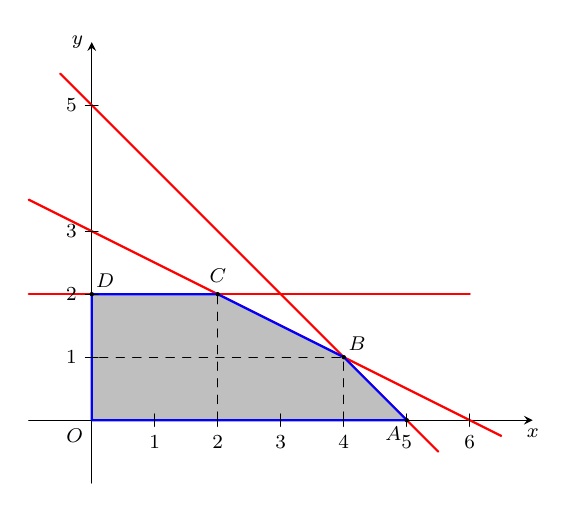
\begin{tikzpicture}[scale=0.8, font=\footnotesize, line join=round, line cap=round, >=stealth]
            \draw[->] (-1,0) -- (7,0) node[below] {$x$};
            \draw[->] (0,-1) -- (0,6) node[left] {$y$};
            \draw (0,0) node [below left] {$O$};
            \draw[thick, red, domain=-0.5:5.5] plot (\x, {5-\x}); % x+y=5
            \draw[thick, red, domain=-1:6.5] plot (\x, {3-0.5*\x}); % x+2y=6
            \draw[thick, red] (-1,2) -- (6,2); % y=2
            \fill[gray!50] (0,0) -- (5,0) -- (4,1) -- (2,2) -- (0,2) -- cycle;
            \draw[thick, blue] (0,0) -- (5,0) -- (4,1) -- (2,2) -- (0,2) -- cycle;
            \path
            (0,0) coordinate (O)
            (5,0) coordinate (A)
            (4,1) coordinate (B)
            (2,2) coordinate (C)
            (0,2) coordinate (D)
            ;
            \foreach \x/\g in {A/-135,B/45,C/90,D/45}
            \fill (\x) circle (1pt) +(\g:0.3) node {$\x$};
            \foreach \x in {1,2,3,4,5,6} \draw (\x,0.1) -- (\x,-0.1) node[below] {$\x$};
            \foreach \y in {1,2,3,5} \draw (0.1,\y) -- (-0.1,\y) node[left] {$\y$};
            \draw[dashed] (4,0) -- (4,1) -- (0,1);
            \draw[dashed] (2,0) -- (2,2);
        \end{tikzpicture}
\end{center}
 Gọi ${x,y}$ lần lượt là số đơn vị sản phẩm loại I, II ($x \ge 0$, $y \ge 0$).

$\begin{cases} 
2 x + 2 y \leq 1 0 \\ 
2 y \leq 4 \\
2 x + 4 y \leq 1 2 
\end{cases}
 \Leftrightarrow \begin{cases}
x+y \leq 5 \\
y \leq 2 \\
x+2 y \leq 6 
\end{cases}$

Gọi $L(x; y)$ là tổng số tiền lãi (đơn vị nghìn đồng), ta có $L(x; y)=3x+5y$.

Biểu diễn miền nghiệm của hệ ta được miền ngũ giác OABCD (kể cả biên) như hình vẽ

Tọa độ các đỉnh của miền ngũ giác là $O(0;0)$, $A(5;0)$, $B(4;1)$, $C(2;2)$, $D(0;2)$.

Tính giá trị của $L(x; y)$ tại các đỉnh được tiền lãi lớn nhất là  $L(B)=17$. 
 }\end{ex}

\begin{ex}
% ID: T10C2B4-281-TLN
% Mức: VDC
 Có ba nhóm máy ${A,B,C}$ dùng để sản xuất ra hai loại sản phẩm ${I}$ và ${II}$. Để sản xuất một đơn vị sản phẩm mỗi loại phải lần lượt dùng các máy thuộc các nhóm khác nhau. Số máy trong một nhóm và số máy của từng nhóm cần thiết để sản xuất ra một đơn vị sản phẩm thuộc mỗi loại được cho trong bảng sau.

Một đơn vị sản phẩm loại I lãi 6 nghìn đồng, một đơn vị sản phẩm loại II lãi 7 nghìn đồng. Trong điều kiện sản xuất đó hãy tính số tiền lãi có thể đạt cao nhất (tiền lãi có đơn vị nghìn đồng).
\begin{center}
\begin{tabular}{|c|c|c|c|}
\hline
\textbf{Nhóm} & \textbf{Số máy trong mỗi nhóm} & \multicolumn{2}{c|}{\textbf{Số máy để sản xuất một đơn vị sản phẩm}} \\ \cline{3-4}
& & \textbf{Loại $I$} & \textbf{Loại $II$} \\ \hline
$A$ & $11$ & $3$ & $3$ \\ \hline
$B$ & $8$ & $0$ & $3$ \\ \hline
$C$ & $20$ & $3$ & $5$ \\ \hline
\end{tabular}


\end{center}


\shortans[4]{24}

\loigiai{ 
 Gọi ${x,y}$ lần lượt là số sản phẩm loại I,II. Điều kiện:

$3x+3y\le 11;\ 3y\le 8;\ 3x+5y\le 20,\ x\ge 0,\ y\ge 0.$

Tiền lãi cần tối ưu:

$P=6x+7y.$

Miền nghiệm có các đỉnh: $(0;0)$, $(0;\frac{8}{3})$, $(1;\frac{8}{3})$, $(\frac{11}{3};0)$.

Tính giá trị biểu thức P tại các đỉnh của miền nghiệm, giá trị lớn nhất là 24. 
 }\end{ex}


\begin{ex}
% ID: T10C2B4-282-TLN
% Mức: VDC
 Người ta định dùng hai loại nguyên liệu để chiết xuất ít nhất 1950 kg hóa chất ${A}$ và 1200 kg hóa chất ${B}$. Từ mỗi tấn nguyên liệu loại I có thể chiết xuất được 600 kg chất ${A}$ và 100 kg chất ${B}$. Từ mỗi tấn nguyên liệu loại II có thể chiết xuất được 300 kg chất ${A}$ và 400 kg chất ${A}$. Biết rằng cơ sở cung cấp nguyên liệu chỉ có thể cung cấp không quá 4 tấn nguyên liệu loại I và 3,5 tấn nguyên liệu loại II, giá tiền mỗi tấn nguyên liệu loại I là 25 triệu đồng, mỗi tấn nguyên liệu loại II là 20 triệu đồng. Hỏi chi phí nhỏ nhất (đơn vị: triệu đồng) để mua nguyên liệu là bao nhiêu (kết quả làm tròn đến hàng phần mười)?


\shortans[4]{100}

\loigiai{ 
 Gọi số tấn nguyên liệu loại I là ${x}$, loại II là ${y}$.

Khi đó $0\le x\le 4.0,\;0\le y\le 3.5$.

Lượng chất A thu được là $600 x + 300 y$, lượng chất B thu được là $100.0 x + 400.0 y$.

Do đó hệ bất phương trình là
$\left\{ \begin{array}{l} 
    0\le x\le 4\\ 
    0\le y\le 3,5\\ 
    2 x + y \geq 6,5\\ 
    0,5 x + 2 y \geq 6 
    \end{array} \right.$

Miền nghiệm là tứ giác có các đỉnh $A(1.5;3.5)$, $B(4.0;3.5)$, $C(4.0;2.0)$, $D(2.0;2.5)$.

Hàm chi phí là $F(x;y)=25 x + 20 y$.

$F(1.5;3.5)=107,5$;
$F(4.0;3.5)=170$;
$F(4.0;2.0)=140$;
$F(2.0;2.5)=100$.

Giá trị nhỏ nhất đạt tại $(2;2,5)$.

Vậy chi phí nhỏ nhất là 100 triệu đồng.

 
 }\end{ex}


\begin{ex}
% ID: T10C2B4-283-TLN
% Mức: VDC
Phòng chăm sóc khách hàng của công ty A làm việc từ 8h00 sáng đến 20h00 mỗi ngày. Nhân viên trực tổng đài làm việc theo 2 ca, mỗi ca 8 tiếng, ca I từ 8h00 đến 16h00 và ca II từ 12h00 đến 20h00. Tiền lương của nhân viên được tính theo giờ (bảng dưới đây). Để chăm sóc khách hàng tốt nhất thì cần tối thiểu 2 nhân viên trong khoảng từ 12h00 -- 20h00, tối thiểu 10 nhân viên trong giờ cao điểm từ 12h00 -- 16h00 và không quá 9 nhân viên trong khoảng từ 8h00 -- 16h00. Do lượng khách hàng trong khoảng 8h00 -- 16h00 thường đông hơn nên phòng chăm sóc khách hàng cần số nhân viên ca I ít nhất phải gấp $1{,}5$ lần số nhân viên ca II. Em hãy giúp công ty A chỉ ra cách huy động số lượng nhân viên cho mỗi ca sao cho chi phí tiền lương mỗi ngày là ít nhất. Khi đó chi phí tiền lương ít nhất mà công ty A phải trả cho nhân viên mỗi ngày là ${{a}}$ (nghìn đồng). Giá trị của ${{a}}$ bằng bao nhiêu?

\begin{center}
\begin{tabular}{|c|c|}
            \hline
            \textbf{Khoảng thời gian làm việc} & \textbf{Tiền lương/giờ} \\            \hline
            8h00 -- 16h00 & 32 000 đồng \\
            \hline
            12h00 -- 20h00 & 30 000 đồng \\
            \hline
        \end{tabular}

\end{center}
\shortans[4]{2496}

\loigiai{
Gọi ${{x}}$ là số nhân viên cần huy động làm ca I và ${{y}}$ là số nhân viên cần huy động làm ca II ($x,y\in\mathbb{N}$).

Theo giả thiết ta có hệ bất phương trình sau:

$\left\{ \begin{array}{l} 
    0<x\le 9 \\ 
    y\ge 2 \\ 
    x+y\ge 10 \\ 
    x\ge 1,5y 
    \end{array} \right.$

 Biểu diễn miền nghiệm của hệ bất phương trình ta được miền nghiệm là miền tứ giác ABCD trong đó $A(6;4)$, $B(8;2)$, $C(9;2)$ và $D(9;6)$.

Chi phí tiền lương mỗi ngày là

$T(x,y)=256x+240y\quad(\text{nghìn đồng}).$

Khi đó giá trị nhỏ nhất của $T(x,y)$ sẽ đạt tại một trong các đỉnh của tứ giác ${{ABCD}}$.

$T(9;2)=2784$, $T(6;4)=2496$, $T(8;2)=2528$, $T(9;6)=3744$.

Do đó chi phí tiền lương mỗi ngày ít nhất khi huy động 6 nhân viên ca I và 4 nhân viên ca II là 2496 (nghìn đồng).
}
\end{ex}

\begin{ex}
% ID: T10C2B4-284-TLN
% Mức: VDC
Phòng chăm sóc khách hàng của công ty A làm việc từ 8h00 sáng đến 20h00 mỗi ngày. Nhân viên trực tổng đài làm việc theo 2 ca, mỗi ca 8 tiếng, ca I từ 8h00 đến 16h00 và ca II từ 12h00 đến 20h00. Tiền lương của nhân viên được tính theo giờ (bảng dưới đây).

Để chăm sóc khách hàng tốt nhất thì cần tối thiểu 2 nhân viên trong khoảng từ 12h00 -- 20h00, tối thiểu ${15}$ nhân viên trong giờ cao điểm từ 12h00 -- 16h00 và không quá ${11}$ nhân viên trong khoảng từ 8h00 -- 16h00. Do lượng khách hàng trong khoảng 8h00 -- 16h00 thường đông hơn nên phòng chăm sóc khách hàng cần số nhân viên ca I ít nhất phải gấp 1,5 lần số nhân viên ca II. Em hãy giúp công ty A chỉ ra cách huy động số lượng nhân viên cho mỗi ca sao cho chi phí tiền lương mỗi ngày là ít nhất. Khi đó chi phí tiền lương ít nhất mà công ty A phải trả cho nhân viên mỗi ngày là ${a}$ (nghìn đồng). Giá trị của ${a}$ bằng bao nhiêu?

\begin{center}
\begin{tabular}{|c|c|}
\hline
\textbf{Khoảng thời gian làm việc} & \textbf{Tiền lương/giờ} \\
\hline
8h00 -- 16h00 & 35000 đồng \\
\hline
12h00 -- 20h00 & 30000 đồng \\
\hline
\end{tabular}
\end{center}
\shortans[4]{495}

\loigiai{
Gọi ${{x}}$ là số nhân viên cần huy động làm ca I và ${{y}}$ là số nhân viên cần huy động làm ca II (${{x,y\in\mathbb{{N}}}}$).

Theo giả thiết ta có hệ bất phương trình:

$\left\{ \begin{array}{l}0<x\le 11 \\y\ge 2 \\x+y\ge 15 \\x\ge 1,5y\end{array} \right.$

Chi phí tiền lương mỗi ngày là

$T(x,y)=35x+30y\quad(\text{nghìn đồng}).$

Do $x\ge 1,5y$ nên tại vị trí chi phí nhỏ nhất ta xét giao điểm $x=1,5y$ và $x+y=15$.

Ta có $1,5y+y=15$, suy ra $y=6$ và $x=9$.

Vậy chi phí tiền lương nhỏ nhất là

$T(9;6)=35\cdot9+30\cdot6=495$ (nghìn đồng).

Do đó chi phí tiền lương mỗi ngày ít nhất là ${495}$ nghìn đồng.
}
\end{ex}
\dangbt{Kiểm tra cặp số là nghiệm của bất phương trình/hệ bất phương trình bậc nhất hai ẩn}
\begin{ex}
 Cho hệ bất phương trình $\left\{ \begin{array}{l}        - x + 2 y + 3 \ge 0\\         - x - 3 y - 2 < 0        \end{array} \right.$. Xét tính đúng-sai của các khẳng định sau.
\choiceTFt
{ $(-3;2)$ không là một nghiệm của hệ bất phương trình }
   { \True $(-2;-3)$ không là nghiệm của hệ bất phương trình }
     { \True $(2;1)$ là một nghiệm của hệ bất phương trình }
    { \True $(4;-5)$ không là nghiệm của hệ bất phương trình }
\loigiai{ 
 

 a) Khẳng định đã cho là khẳng định sai.

 Thay $(-3;2)$ vào thấy thỏa mãn nên $(-3;2)$ là một nghiệm của hệ bất phương trình.

b) Khẳng định đã cho là khẳng định đúng.

 Thay $(-2;-3)$ vào thấy không thỏa mãn nên $(-2;-3)$ không là nghiệm của hệ bất phương trình.

c) Khẳng định đã cho là khẳng định đúng.

 Thay $(2;1)$  vào thấy thỏa mãn nên $(2;1)$ là một nghiệm của hệ bất phương trình.

d) Khẳng định đã cho là khẳng định đúng.

 Thay $(4;-5)$ vào thấy thỏa mãn nên $(4;-5)$ là một nghiệm của hệ bất phương trình.

 
 }\end{ex}

\dangbt{Kiểm tra cặp số là nghiệm của bất phương trình/hệ bất phương trình bậc nhất hai ẩn}
\begin{ex}Cho hệ bất phương trình $\left\{ \begin{array}{l}        - 2 x + 3 y + 4 > 0\\         x - 2 y + 4 < 0        \end{array} \right.$. Xét tính đúng-sai của các khẳng định sau.
\choiceTF
{ \True $(-5;1)$ là một nghiệm của hệ bất phương trình }
   { \True $(0;-2)$ không là nghiệm của hệ bất phương trình }
     { $(2;4)$ không là nghiệm của hệ bất phương trình }
    { $(4;2)$ là một nghiệm của hệ bất phương trình }
\loigiai{
a) Khẳng định đã cho là khẳng định đúng.
 Thay $(-5;1)$ vào thấy thỏa mãn nên $(-5;1)$ là một nghiệm của hệ bất phương trình.
b) Khẳng định đã cho là khẳng định đúng.
 Thay $(0;-2)$ vào thấy không thỏa mãn nên $(0;-2)$ không là nghiệm của hệ bất phương trình.
c) Khẳng định đã cho là khẳng định sai.
 Thay $(2;4)$  vào thấy thỏa mãn nên $(2;4)$ là một nghiệm của hệ bất phương trình.
d) Khẳng định đã cho là khẳng định sai.
 Thay $(4;2)$ vào thấy thỏa mãn nên $(4;2)$ là một nghiệm của hệ bất phương trình.
}
\end{ex}

\dangbt{Kiểm tra cặp số là nghiệm của bất phương trình/hệ bất phương trình bậc nhất hai ẩn}
\begin{ex}Cho hệ bất phương trình $\left\{ \begin{array}{l}        2 x + 3 y - 5 > 0\\         - 3 x + y - 5 > 0        \end{array} \right.$. Xét tính đúng-sai của các khẳng định sau.
\choiceTF
{ $(-3;6)$ không là một nghiệm của hệ bất phương trình }
   { $(0;0)$ là một nghiệm của hệ bất phương trình  }
     { \True $(2;14)$ là một nghiệm của hệ bất phương trình }
    { $(4;15)$ là một nghiệm của hệ bất phương trình }
\loigiai{
a) Khẳng định đã cho là khẳng định sai.
 Thay $(-3;6)$ vào thấy thỏa mãn nên $(-3;6)$ là một nghiệm của hệ bất phương trình.
b) Khẳng định đã cho là khẳng định sai.
 Thay $(0;0)$ vào thấy không thỏa mãn nên $(0;0)$ không là nghiệm của hệ bất phương trình.
c) Khẳng định đã cho là khẳng định đúng.
 Thay $(2;14)$  vào thấy thỏa mãn nên $(2;14)$ là một nghiệm của hệ bất phương trình.
d) Khẳng định đã cho là khẳng định sai.
 Thay $(4;15)$ vào thấy thỏa mãn nên $(4;15)$ là một nghiệm của hệ bất phương trình.
}
\end{ex}

\dangbt{Kiểm tra cặp số là nghiệm của bất phương trình/hệ bất phương trình bậc nhất hai ẩn}
\begin{ex}
 Cho hệ bất phương trình $\left\{ \begin{array}{l}        x + 3 y + 2 \ge 0\\         - 3 x + y + 4 \ge 0        \end{array} \right.$. Xét tính đúng-sai của các khẳng định sau.
\choiceTFt
{ $(-4;3)$ không là một nghiệm của hệ bất phương trình }
   { \True $(-2;-1)$ không là nghiệm của hệ bất phương trình }
     { \True $(1;2)$ là một nghiệm của hệ bất phương trình }
    { \True $(4;7)$ không là nghiệm của hệ bất phương trình }
\loigiai{ 
 

 a) Khẳng định đã cho là khẳng định sai.

 Thay $(-4;3)$ vào thấy thỏa mãn nên $(-4;3)$ là một nghiệm của hệ bất phương trình.

b) Khẳng định đã cho là khẳng định đúng.

 Thay $(-2;-1)$ vào thấy không thỏa mãn nên $(-2;-1)$ không là nghiệm của hệ bất phương trình.

c) Khẳng định đã cho là khẳng định đúng.

 Thay $(1;2)$  vào thấy thỏa mãn nên $(1;2)$ là một nghiệm của hệ bất phương trình.

d) Khẳng định đã cho là khẳng định đúng.

 Thay $(4;7)$ vào thấy thỏa mãn nên $(4;7)$ là một nghiệm của hệ bất phương trình.

 
 }\end{ex}

\dangbt{Kiểm tra cặp số là nghiệm của bất phương trình/hệ bất phương trình bậc nhất hai ẩn}
\begin{ex}
 Chú Minh dự định trồng lúa và khoai lang trên một mảnh đất có diện tích 9 sào. Nếu trồng 1 sào lúa thì cần 4 ngày công và thu được 5 triệu đồng. Nếu trồng 1 sào khoai lang thì cần 5 ngày công và thu được 8 triệu đồng. Tổng số ngày công mà Chú Minh có thể sử dụng không quá 40 ngày công. Gọi ${x, y}$ lần lượt là diện tích đất trồng lúa và khoai lang (đơn vị: sào). Xét tính đúng-sai của các khẳng định sau:
\choiceTFt
{  Tổng diện tích đất cần dùng là $4x+5y$ }
   { $x+y \ge 9$ }
     { \True $4x+5y \le 40$ }
    { Lợi nhuận lớn nhất thu được là 68 triệu đồng }
\loigiai{ 
 

 a) Khẳng định đã cho là khẳng định sai.

 Tổng diện tích đất cần dùng là $x+y$

b) Khẳng định đã cho là khẳng định sai.

 $x+y \le 9$.

c) Khẳng định đã cho là khẳng định đúng.

 $4x+5y \le 40$.

d) Khẳng định đã cho là khẳng định sai.

 Gọi ${x,y}$ là diện tích đất để trồng lúa và khoai lang.

$x\ge 0,y \ge 0$.

Diện tích đất cần dùng: $x+y \le 9$.

Số ngày công cần dùng: $4x+5y \le 40$.

Miền nghiệm của hệ điều kiện là tứ giác ${OABC}$với $O(0;0),A(0;8),B(5;4),C(9;0)$.

Lợi nhuận thu được: $F=5x+8y$.

$F(0;0)=0, F(0;8)=64, F(5;4)=57, F(9;0)=45$.

 Điểm thỏa mãn lợi nhuận lớn nhất:  $x = 0, y = 8$

 Lợi nhuận lớn nhất: F = 64 triệu đồng.

 
 }\end{ex}

\dangbt{Kiểm tra cặp số là nghiệm của bất phương trình/hệ bất phương trình bậc nhất hai ẩn}
\begin{ex}
 Bác Hùng dự định trồng cà chua và dưa leo trên một mảnh đất có diện tích 6 sào. Nếu trồng 1 sào cà chua thì cần 3 ngày công và thu được 10 triệu đồng. Nếu trồng 1 sào dưa leo thì cần 8 ngày công và thu được 6 triệu đồng. Tổng số ngày công mà Bác Hùng có thể sử dụng không quá 24 ngày công. Gọi ${x, y}$ lần lượt là diện tích đất trồng cà chua và dưa leo (đơn vị: sào). Xét tính đúng-sai của các khẳng định sau:
\choiceTFt
{ \True  Tổng diện tích đất cần dùng là $x+y$ }
   { \True $x+y \le 6$ }
     { \True $3x+8y \le 24$ }
    { \True  Lợi nhuận lớn nhất thu được là 60 triệu đồng }
\loigiai{ 
 

 a) Khẳng định đã cho là khẳng định đúng.

 Tổng diện tích đất cần dùng là $x+y$

b) Khẳng định đã cho là khẳng định đúng.

 $x+y \le 6$.

c) Khẳng định đã cho là khẳng định đúng.

 $3x+8y \le 24$.

d) Khẳng định đã cho là khẳng định đúng.

 Gọi ${x,y}$ là diện tích đất để trồng cà chua và dưa leo.

$x\ge 0,y \ge 0$.

Diện tích đất cần dùng: $x+y \le 6$.

Số ngày công cần dùng: $3x+8y \le 24$.

Miền nghiệm của hệ điều kiện là tứ giác ${OABC}$với $O(0;0),A(0;3),B(\frac{24}{5};\frac{6}{5}),C(6;0)$.

Lợi nhuận thu được: $F=10x+6y$.

$F(0;0)=0, F(0;3)=18, F(\frac{24}{5};\frac{6}{5})=55, F(6;0)=60$.

 Điểm thỏa mãn lợi nhuận lớn nhất:  $x = 6, y = 0$

 Lợi nhuận lớn nhất: F = 60 triệu đồng.

 
 }\end{ex}

\dangbt{Kiểm tra cặp số là nghiệm của bất phương trình/hệ bất phương trình bậc nhất hai ẩn}
\begin{ex}
 Bạn Hoa dự định làm thủ công các bao lì xì để bán trong một hội chợ Tết. Cần 6 giờ để làm một bao lì xì đặc biệt có giá 22 nghìn đồng và 3 giờ để làm một bao lì xì thường có giá 8 nghìn đồng. Bạn Hoa chỉ có 36 giờ để làm các bao lì xì và ban tổ chức hội chợ yêu cầu phải làm ít nhất 10 bao lì xì. Gọi ${x,y}$ lần lượt là số lượng bao lì xì đặc biệt và bao lì xì thường. Xét tính đúng-sai của các khẳng định sau. 
\choiceTFt
{ \True  $x+y \ge 10$ }
   {  $6x+3y \ge 36$ }
     { \True  Với $x = 2, y = 8$ thì số tiền thu về là lớn nhất }
    { \True  Số tiền có thể thu về được nhiều nhất khi bán hết các bao lì xì là 108 ngàn đồng }
\loigiai{ 
 

 a) Khẳng định đã cho là khẳng định đúng.

 $x+y \ge 10$.

b) Khẳng định đã cho là khẳng định sai.

 $6x+3y \le 36$.

c) Khẳng định đã cho là khẳng định đúng.

 Gọi ${x,y}$ là số lượng bao lì xì đặc biệt và bao lì xì thường.

$x\ge 0,y \ge 0$.

Số lượng bao lì xì cần làm: $x+y \ge 10$.

Số giờ cần dùng: $6x+3y \le 36$.

Miền nghiệm của hệ điều kiện là tam giác ${ABC}$ với $A(0;10),B(2;8),C(0;12)$.

$F (2, 8) = 108$

$F (0, 10) = 80$

$F (0, 12) = 96$



Lợi nhuận thu được: $F=22x+8y$.

Số tiền thu về lớn nhất khi:  $x = 2, y = 8$.

d) Khẳng định đã cho là khẳng định đúng.

 Số tiền có thể thu về được nhiều nhất: F(2,8) = 108 ngàn đồng.

 
 }\end{ex}

\dangbt{Kiểm tra cặp số là nghiệm của bất phương trình/hệ bất phương trình bậc nhất hai ẩn}
\begin{ex}
 Một xưởng sản xuất có hai máy đặc chủng là máy A và máy B để sản xuất hai loại sản phẩm X và Y. Để sản xuất 1 tấn sản phẩm loại X cần dùng máy A trong 2 giờ và dùng máy B trong 1 giờ. Để sản xuất 1 tấn sản phẩm loại Y cần dùng máy A trong 1 giờ và dùng máy B trong 2 giờ. Cho biết mỗi máy không thể sản xuất đồng thời hai loại sản phẩm. Máy A làm việc không quá 7 giờ một ngày, máy B làm việc không quá 8 giờ một ngày. Một cái X lãi 6 triệu đồng và một sản phẩm loại Y lãi 3 triệu đồng. Gọi ${x,y}$ lần lượt là số tấn sản phẩm loại X và loại Y cần sản xuất. Xét tính đúng-sai của các khẳng định sau:
\choiceTFt
{ \True  $2 x + y - 7 \le 0$ }
   { \True  $x + 2 y - 8 \le 0$ }
     { \True  Với $x = 2, y = 3$ thì lợi nhuận thu được là lớn nhất }
    { Lợi nhuận lớn nhất đạt được là 26 triệu đồng  }
\loigiai{ 
 

 a) Khẳng định đã cho là khẳng định đúng.

 Thời gian để máy A làm việc: $2 x + y - 7 \le 0$.

b) Khẳng định đã cho là khẳng định đúng.

 Thời gian để máy B làm việc: $x + 2 y - 8 \le 0$.

c) Khẳng định đã cho là khẳng định đúng.

 Gọi ${x}$, ${y}$ là số tấn sản phẩm loại ${X}$, ${Y}$ cần sản xuất ($ x,y\ge 0 $).

Thời gian để máy A làm việc: $2 x + y \le 7$.

Thời gian để máy B làm việc: $x + 2 y \le 8$.

Ta có hệ điều kiện:

$\left\{ \begin{array}{l} 
    2 x + y\le 7 \\ 
    x + 2 y\le 8 \\ 
    x \ge 0 \\ 
    y \ge 0 
    \end{array} \right.$.

Lợi nhuận thu được: $T=6 x + 3 y$.

 Lợi nhuận tại các đỉnh của miền nghiệm:

 $T(2, 3) = 21$

$T(\frac{7}{2}, 0) = 21$

$T(0, 4) = 12$

$T(0, 0) = 0$



 Điểm thỏa mãn lợi nhuận lớn nhất:  $x = 2, y = 3$



d) Khẳng định đã cho là khẳng định sai.

 Lợi nhuận lớn nhất đạt được là $F(2,3)=21$ triệu đồng.

 
 }\end{ex}
\dangbt{Bài toán tối ưu hóa (tìm GTLN/GTNN) trên miền nghiệm}
\begin{ex}
Cho biểu thức $F=4 x - 2 y$ với $(x;y)$ là các điểm thuộc miền trong hình tứ giác như hình vẽ. Tìm khẳng định đúng.
\choice
{A. $F_{max} = 12$}
{B. $F_{min} = -2$}
{\True C. $F_{max} = 16$}
{D. $F_{min} = -4$}
\loigiai{Để tìm giá trị lớn nhất và nhỏ nhất của biểu thức $F=4x-2y$ trên miền tứ giác, ta cần xác định tọa độ các đỉnh của tứ giác và thay vào biểu thức $F$.
Giả sử các đỉnh của tứ giác là:
$A(x_A, y_A)$, $B(x_B, y_B)$, $C(x_C, y_C)$, $D(x_D, y_D)$.
Từ hình vẽ, ta có thể ước lượng các tọa độ đỉnh (cần hình vẽ cụ thể để xác định chính xác):
Ví dụ: $A(4,0)$, $B(5,2)$, $C(2,3)$, $D(0,1)$.
Tính giá trị $F$ tại các đỉnh:
$F(A) = 4(4) - 2(0) = 16$
$F(B) = 4(5) - 2(2) = 20 - 4 = 16$
$F(C) = 4(2) - 2(3) = 8 - 6 = 2$
$F(D) = 4(0) - 2(1) = -2$
Từ các giá trị này, ta thấy:
$F_{max} = 16$ (đạt tại $A(4,0)$ và $B(5,2)$)
$F_{min} = -2$ (đạt tại $D(0,1)$)
So sánh với các phương án:
A. $F_{max} = 12$ (Sai)
B. $F_{min} = -2$ (Đúng)
C. $F_{max} = 16$ (Đúng)
D. $F_{min} = -4$ (Sai)
Vì có hai đáp án B và C đều đúng, ta cần kiểm tra lại đề bài hoặc hình vẽ để đảm bảo tính duy nhất của đáp án. Tuy nhiên, nếu phải chọn một, và $F_{max}$ thường là mục tiêu chính trong các bài tối ưu hóa, ta chọn C.
Chọn C.}
\end{ex}

\dangbt{Kiểm tra tính đúng sai của các khẳng định về bất phương trình/hệ bất phương trình bậc nhất hai ẩn và bài toán thực tế}
\begin{ex}
Xét bất phương trình $- 3 x + 3 y - 3\ge 0$. Xét tính đúng-sai của các khẳng định sau.
\choiceTF
{\True A. Cặp số $(1;2)$ là một nghiệm của bất phương trình.}
{B. Cặp số $(0;0)$ là một nghiệm của bất phương trình.}
{C. Miền nghiệm của bất phương trình là nửa mặt phẳng không chứa điểm $(1;0)$.}
{D. Đường thẳng $-3x+3y-3=0$ không phải là đường biên của miền nghiệm.}
\loigiai{a đúng vì thay $(1;2)$ vào bất phương trình: $-3(1)+3(2)-3 = -3+6-3 = 0 \ge 0$.
b sai vì thay $(0;0)$ vào bất phương trình: $-3(0)+3(0)-3 = -3 \not\ge 0$.
c sai vì điểm $(1;0)$ có $-3(1)+3(0)-3 = -6 \not\ge 0$, nên miền nghiệm không chứa $(1;0)$. Phát biểu "không chứa điểm $(1;0)$" là đúng, nhưng câu hỏi là "Miền nghiệm của bất phương trình là nửa mặt phẳng không chứa điểm $(1;0)$", điều này không đủ để khẳng định tính đúng sai của miền nghiệm. Miền nghiệm là nửa mặt phẳng chứa các điểm thỏa mãn bất phương trình.
d sai vì đường thẳng $-3x+3y-3=0$ chính là đường biên của miền nghiệm của bất phương trình $-3x+3y-3 \ge 0$ (do có dấu bằng).
Chọn A.}
\end{ex}
\dangbt{Kiểm tra cặp số là nghiệm của bất phương trình/hệ bất phương trình bậc nhất hai ẩn}
\begin{ex}
Cho hệ bất phương trình bậc nhất hai ẩn
\\(\begin{cases} 3x + 2y \ge -6 \\ x + 4y > 4. \end{cases}\\)
Xét tính đúng sai của các khẳng định sau:
\choiceTF
{\True Cặp số \\((0;2)\\) là một nghiệm của hệ bất phương trình đã cho.}
{Cặp số \\((1;0)\\) là một nghiệm của hệ bất phương trình đã cho.}
{\True Cặp số \\((-1;2)\\) là một nghiệm của hệ bất phương trình đã cho.}
{Cặp số \\((0;0)\\) là một nghiệm của hệ bất phương trình đã cho.}
\loigiai{
- Thay cặp số \\((0;2)\\) vào hệ ta được: \\(3 \cdot 0 + 2 \cdot 2 = 4 \ge -6\\) (đúng) và \\(0 + 4 \cdot 2 = 8 > 4\\) (đúng). Vậy \\((0;2)\\) là nghiệm của hệ.
- Thay cặp số \\((1;0)\\) vào hệ ta được: \\(3 \cdot 1 + 2 \cdot 0 = 3 \ge -6\\) (đúng) nhưng \\(1 + 4 \cdot 0 = 1 > 4\\) (sai). Vậy \\((1;0)\\) không phải là nghiệm của hệ.
- Thay cặp số \\((-1;2)\\) vào hệ ta được: \\(3 \cdot (-1) + 2 \cdot 2 = 1 \ge -6\\) (đúng) và \\(-1 + 4 \cdot 2 = 7 > 4\\) (đúng). Vậy \\((-1;2)\\) là nghiệm của hệ.
- Thay cặp số \\((0;0)\\) vào hệ ta được: \\(0 + 4 \cdot 0 = 0 > 4\\) (sai). Vậy \\((0;0)\\) không phải là nghiệm của hệ.
}
\end{ex}
